%%%%%%%%%%%%%%%%%%%%%%%%%%%%%%%%%%%%%%%%%
% The Legrand Orange Book
% LaTeX Template
% Version 1.4 (12/4/14)
%
% This template has been downloaded from:
% http://www.LaTeXTemplates.com
%
% Original author:
% Mathias Legrand (legrand.mathias@gmail.com)
%
% License:
% CC BY-NC-SA 3.0 (http://creativecommons.org/licenses/by-nc-sa/3.0/)
%
% Compiling this template:
% This template uses biber for its bibliography and makeindex for its index.
% When you first open the template, compile it from the command line with the 
% commands below to make sure your LaTeX distribution is configured correctly:
%
% 1) pdflatex oqhbt
% 2) makeindex oqhbt.idx -s StyleInd.ist
% 3) biber oqhbt
% 4  makeglossaries oqhbt
% 4) pdflatex oqhbt x 2
%
% After this, when you wish to update the bibliography/index use the appropriate
% command above and make sure to compile with pdflatex several times 
% afterwards to propagate your changes to the document.
%
% This template also uses a number of packages which may need to be
% updated to the newest versions for the template to compile. It is strongly
% recommended you update your LaTeX distribution if you have any
% compilation errors.
%
% Important note:
% Chapter heading images should have a 2:1 width:height ratio,
% e.g. 920px width and 460px height.
%
%%%%%%%%%%%%%%%%%%%%%%%%%%%%%%%%%%%%%%%%%

%----------------------------------------------------------------------------------------
%	PACKAGES AND OTHER DOCUMENT CONFIGURATIONS
%----------------------------------------------------------------------------------------

\documentclass[11pt,fleqn]{book} % Default font size and left-justified equations

\usepackage[top=3cm,bottom=3cm,left=3.2cm,right=3.2cm,headsep=10pt,a4paper]{geometry} % Page margins

\usepackage{xcolor} % Required for specifying colors by name
\definecolor{ocre}{RGB}{243,102,25} % Define the orange color used for highlighting throughout the book
\usepackage{setspace}

% Font Settings
\usepackage{avant} % Use the Avantgarde font for headings
%\usepackage{times} % Use the Times font for headings
\usepackage{mathptmx} % Use the Adobe Times Roman as the default text font together with math symbols from the Sym­bol, Chancery and Com­puter Modern fonts

\usepackage{microtype} % Slightly tweak font spacing for aesthetics
\usepackage[utf8]{inputenc} % Required for including letters with accents
\usepackage[T1]{fontenc} % Use 8-bit encoding that has 256 glyphs

% Bibliography
\usepackage[style=alphabetic,
            sorting=nyt,
            sortcites=true,
            natbib=true,
            style=authoryear,
            maxcitenames=2,
            maxbibnames=100,
            autopunct=true,
            babel=hyphen,
            hyperref=true,
            doi=true,
            abbreviate=false,
            backref=true,
            backend=biber]{biblatex}
\addbibresource{./bibliography/gmpe_smtk_biblio.bib} % BibTeX bibliography file
\defbibheading{bibempty}{}

% Figure caption settings
\usepackage[textfont=it,margin=10pt,font=small,labelfont=bf,labelsep=endash]{caption}

% Table
\usepackage{color, colortbl}
\definecolor{almond}{rgb}{0.94, 0.87, 0.8}
\definecolor{ashgrey}{rgb}{0.7, 0.75, 0.71}
\definecolor{anti-flashwhite}{rgb}{0.95, 0.95, 0.96}

% Index
\usepackage{calc} % For simpler calculation - used for spacing the index letter headings correctly
\usepackage{makeidx} % Required to make an index
\makeindex % Tells LaTeX to create the files required for indexing

\usepackage{todonotes}

%
% Package to create a glossary - It must be uploaded after hyperref
% to produce the glossary: makeglossaries OQB
\usepackage[acronym,nonumberlist,style=altlist]{glossaries}
\glstoctrue
\makeglossaries

% package for bold symbols
\usepackage{bm}

%----------------------------------------------------------------------------------------
% Insert the commands.tex file which contains the majority of the structure 
% behind the template
%----------------------------------------------------------------------------------------
%	VARIOUS REQUIRED PACKAGES
%----------------------------------------------------------------------------------------

\usepackage{titlesec} % Allows customization of titles

\usepackage{graphicx} % Required for including pictures
\graphicspath{{Pictures/}} % Specifies the directory where pictures are stored

\usepackage{tikz} % Required for drawing custom shapes

\usepackage[english]{babel} % English language/hyphenation

\usepackage{enumitem} % Customize lists
\setlist{nolistsep} % Reduce spacing between bullet points and numbered lists

\usepackage{booktabs} % Required for nicer horizontal rules in tables

\usepackage{eso-pic} % Required for specifying an image background in the title page

%----------------------------------------------------------------------------------------
%	MAIN TABLE OF CONTENTS
%----------------------------------------------------------------------------------------

\usepackage{titletoc} % Required for manipulating the table of contents

\contentsmargin{0cm} % Removes the default margin
% Chapter text styling
\titlecontents{chapter}[1.25cm] % Indentation
{\addvspace{15pt}\large\sffamily\bfseries} % Spacing and font options for chapters
{\color{ocre!60}\contentslabel[\Large\thecontentslabel]{1.25cm}\color{ocre}} % Chapter number
{}  
{\color{ocre!60}\normalsize\sffamily\bfseries\;\titlerule*[.5pc]{.}\;\thecontentspage} % Page number
% Section text styling
\titlecontents{section}[1.25cm] % Indentation
{\addvspace{5pt}\sffamily\bfseries} % Spacing and font options for sections
{\contentslabel[\thecontentslabel]{1.25cm}} % Section number
{}
{\sffamily\hfill\color{black}\thecontentspage} % Page number
[]
% Subsection text styling
\titlecontents{subsection}[1.25cm] % Indentation
{\addvspace{1pt}\sffamily\small} % Spacing and font options for subsections
{\contentslabel[\thecontentslabel]{1.25cm}} % Subsection number
{}
{\sffamily\;\titlerule*[.5pc]{.}\;\thecontentspage} % Page number
[] 

%----------------------------------------------------------------------------------------
%	MINI TABLE OF CONTENTS IN CHAPTER HEADS
%----------------------------------------------------------------------------------------

% Section text styling
\titlecontents{lsection}[0em] % Indendating
{\footnotesize\sffamily} % Font settings
{}
{}
{}

% Subsection text styling
\titlecontents{lsubsection}[.5em] % Indentation
{\normalfont\footnotesize\sffamily} % Font settings
{}
{}
{}
 
%----------------------------------------------------------------------------------------
%	PAGE HEADERS
%----------------------------------------------------------------------------------------

\usepackage{fancyhdr} % Required for header and footer configuration

\pagestyle{fancy}
\renewcommand{\chaptermark}[1]{\markboth{\sffamily\normalsize\bfseries\chaptername\ \thechapter.\ #1}{}} % Chapter text font settings
\renewcommand{\sectionmark}[1]{\markright{\sffamily\normalsize\thesection\hspace{5pt}#1}{}} % Section text font settings
\fancyhf{} \fancyhead[LE,RO]{\sffamily\normalsize\thepage} % Font setting for the page number in the header
\fancyhead[LO]{\rightmark} % Print the nearest section name on the left side of odd pages
\fancyhead[RE]{\leftmark} % Print the current chapter name on the right side of even pages
\renewcommand{\headrulewidth}{0.5pt} % Width of the rule under the header
\addtolength{\headheight}{2.5pt} % Increase the spacing around the header slightly
\renewcommand{\footrulewidth}{0pt} % Removes the rule in the footer
\fancypagestyle{plain}{\fancyhead{}\renewcommand{\headrulewidth}{0pt}} % Style for when a plain pagestyle is specified

% Removes the header from odd empty pages at the end of chapters
\makeatletter
\renewcommand{\cleardoublepage}{
\clearpage\ifodd\c@page\else
\hbox{}
\vspace*{\fill}
\thispagestyle{empty}
\newpage
\fi}

%----------------------------------------------------------------------------------------
%	THEOREM STYLES
%----------------------------------------------------------------------------------------

\usepackage{amsmath,amsfonts,amssymb,amsthm} % For math equations, theorems, symbols, etc

\newcommand{\intoo}[2]{\mathopen{]}#1\,;#2\mathclose{[}}
\newcommand{\ud}{\mathop{\mathrm{{}d}}\mathopen{}}
\newcommand{\intff}[2]{\mathopen{[}#1\,;#2\mathclose{]}}
\newtheorem{notation}{Notation}[chapter]

%%%%%%%%%%%%%%%%%%%%%%%%%%%%%%%%%%%%%%%%%%%%%%%%%%%%%%%%%%%%%%%%%%%%%%%%%%%
%%%%%%%%%%%%%%%%%%%% dedicated to boxed/framed environements %%%%%%%%%%%%%%
%%%%%%%%%%%%%%%%%%%%%%%%%%%%%%%%%%%%%%%%%%%%%%%%%%%%%%%%%%%%%%%%%%%%%%%%%%%
\newtheoremstyle{ocrenumbox}% % Theorem style name
{0pt}% Space above
{0pt}% Space below
{\normalfont}% % Body font
{}% Indent amount
{\small\bf\sffamily\color{ocre}}% % Theorem head font
{\;}% Punctuation after theorem head
{0.25em}% Space after theorem head
{\small\sffamily\color{ocre}\thmname{#1}\nobreakspace\thmnumber{\@ifnotempty{#1}{}\@upn{#2}}% Theorem text (e.g. Theorem 2.1)
\thmnote{\nobreakspace\the\thm@notefont\sffamily\bfseries\color{black}---\nobreakspace#3.}} % Optional theorem note
\renewcommand{\qedsymbol}{$\blacksquare$}% Optional qed square

\newtheoremstyle{blacknumex}% Theorem style name
{5pt}% Space above
{5pt}% Space below
{\normalfont}% Body font
{} % Indent amount
{\small\bf\sffamily}% Theorem head font
{\;}% Punctuation after theorem head
{0.25em}% Space after theorem head
{\small\sffamily{\tiny\ensuremath{\blacksquare}}\nobreakspace\thmname{#1}\nobreakspace\thmnumber{\@ifnotempty{#1}{}\@upn{#2}}% Theorem text (e.g. Theorem 2.1)
\thmnote{\nobreakspace\the\thm@notefont\sffamily\bfseries---\nobreakspace#3.}}% Optional theorem note

\newtheoremstyle{blacknumbox} % Theorem style name
{0pt}% Space above
{0pt}% Space below
{\normalfont}% Body font
{}% Indent amount
{\small\bf\sffamily}% Theorem head font
{\;}% Punctuation after theorem head
{0.25em}% Space after theorem head
{\small\sffamily\thmname{#1}\nobreakspace\thmnumber{\@ifnotempty{#1}{}\@upn{#2}}% Theorem text (e.g. Theorem 2.1)
\thmnote{\nobreakspace\the\thm@notefont\sffamily\bfseries---\nobreakspace#3.}}% Optional theorem note

%%%%%%%%%%%%%%%%%%%%%%%%%%%%%%%%%%%%%%%%%%%%%%%%%%%%%%%%%%%%%%%%%%%%%%%%%%%
%%%%%%%%%%%%% dedicated to non-boxed/non-framed environements %%%%%%%%%%%%%
%%%%%%%%%%%%%%%%%%%%%%%%%%%%%%%%%%%%%%%%%%%%%%%%%%%%%%%%%%%%%%%%%%%%%%%%%%%
\newtheoremstyle{ocrenum}% % Theorem style name
{5pt}% Space above
{5pt}% Space below
{\normalfont}% % Body font
{}% Indent amount
{\small\bf\sffamily\color{ocre}}% % Theorem head font
{\;}% Punctuation after theorem head
{0.25em}% Space after theorem head
{\small\sffamily\color{ocre}\thmname{#1}\nobreakspace\thmnumber{\@ifnotempty{#1}{}\@upn{#2}}% Theorem text (e.g. Theorem 2.1)
\thmnote{\nobreakspace\the\thm@notefont\sffamily\bfseries\color{black}---\nobreakspace#3.}} % Optional theorem note
\renewcommand{\qedsymbol}{$\blacksquare$}% Optional qed square
\makeatother

% Defines the theorem text style for each type of theorem to one of the three styles above
\newcounter{dummy} 
\numberwithin{dummy}{section}
\theoremstyle{ocrenumbox}
\newtheorem{theoremeT}[dummy]{Theorem}
\newtheorem{problem}{Problem}[chapter]
\newtheorem{exerciseT}{Exercise}[chapter]
\theoremstyle{blacknumex}
\newtheorem{exampleT}{Example}[chapter]
\theoremstyle{blacknumbox}
\newtheorem{vocabulary}{Vocabulary}[chapter]
\newtheorem{definitionT}{Definition}[section]
\newtheorem{corollaryT}[dummy]{Corollary}
\theoremstyle{ocrenum}
\newtheorem{proposition}[dummy]{Proposition}

%----------------------------------------------------------------------------------------
%	DEFINITION OF COLORED BOXES
%----------------------------------------------------------------------------------------

\RequirePackage[framemethod=default]{mdframed} % Required for creating the theorem, definition, exercise and corollary boxes

% Theorem box
\newmdenv[skipabove=7pt,
skipbelow=7pt,
backgroundcolor=black!5,
linecolor=ocre,
innerleftmargin=5pt,
innerrightmargin=5pt,
innertopmargin=5pt,
leftmargin=0cm,
rightmargin=0cm,
innerbottommargin=5pt]{tBox}

% Exercise box	  
\newmdenv[skipabove=7pt,
skipbelow=7pt,
rightline=false,
leftline=true,
topline=false,
bottomline=false,
backgroundcolor=ocre!10,
linecolor=ocre,
innerleftmargin=5pt,
innerrightmargin=5pt,
innertopmargin=5pt,
innerbottommargin=5pt,
leftmargin=0cm,
rightmargin=0cm,
linewidth=4pt]{eBox}	

% Definition box
\newmdenv[skipabove=7pt,
skipbelow=7pt,
rightline=false,
leftline=true,
topline=false,
bottomline=false,
linecolor=ocre,
innerleftmargin=5pt,
innerrightmargin=5pt,
innertopmargin=0pt,
leftmargin=0cm,
rightmargin=0cm,
linewidth=4pt,
innerbottommargin=0pt]{dBox}	

% Corollary box
\newmdenv[skipabove=7pt,
skipbelow=7pt,
rightline=false,
leftline=true,
topline=false,
bottomline=false,
linecolor=gray,
backgroundcolor=black!5,
innerleftmargin=5pt,
innerrightmargin=5pt,
innertopmargin=5pt,
leftmargin=0cm,
rightmargin=0cm,
linewidth=4pt,
innerbottommargin=5pt]{cBox}

% Creates an environment for each type of theorem and assigns it a theorem text style from the "Theorem Styles" section above and a colored box from above
\newenvironment{theorem}{\begin{tBox}\begin{theoremeT}}{\end{theoremeT}\end{tBox}}
\newenvironment{exercise}{\begin{eBox}\begin{exerciseT}}{\hfill{\color{ocre}\tiny\ensuremath{\blacksquare}}\end{exerciseT}\end{eBox}}				  
\newenvironment{definition}{\begin{dBox}\begin{definitionT}}{\end{definitionT}\end{dBox}}	
\newenvironment{example}{\begin{exampleT}}{\hfill{\tiny\ensuremath{\blacksquare}}\end{exampleT}}		
\newenvironment{corollary}{\begin{cBox}\begin{corollaryT}}{\end{corollaryT}\end{cBox}}	

%----------------------------------------------------------------------------------------
%	REMARK ENVIRONMENT
%----------------------------------------------------------------------------------------

\newenvironment{remark}{\par\vspace{10pt}\small % Vertical white space above the remark and smaller font size
\begin{list}{}{
\leftmargin=35pt % Indentation on the left
\rightmargin=25pt}\item\ignorespaces % Indentation on the right
\makebox[-2.5pt]{\begin{tikzpicture}[overlay]
\node[draw=ocre!60,line width=1pt,circle,fill=ocre!25,font=\sffamily\bfseries,inner sep=2pt,outer sep=0pt] at (-15pt,0pt){\textcolor{ocre}{R}};\end{tikzpicture}} % Orange R in a circle
\advance\baselineskip -1pt}{\end{list}\vskip5pt} % Tighter line spacing and white space after remark

%----------------------------------------------------------------------------------------
%	SECTION NUMBERING IN THE MARGIN
%----------------------------------------------------------------------------------------

\makeatletter
\renewcommand{\@seccntformat}[1]{\llap{\textcolor{ocre}{\csname the#1\endcsname}\hspace{1em}}}                    
\renewcommand{\section}{\@startsection{section}{1}{\z@}
{-4ex \@plus -1ex \@minus -.4ex}
{1ex \@plus.2ex }
{\normalfont\large\sffamily\bfseries}}
\renewcommand{\subsection}{\@startsection {subsection}{2}{\z@}
{-3ex \@plus -0.1ex \@minus -.4ex}
{0.5ex \@plus.2ex }
{\normalfont\sffamily\bfseries}}
\renewcommand{\subsubsection}{\@startsection {subsubsection}{3}{\z@}
{-2ex \@plus -0.1ex \@minus -.2ex}
{.2ex \@plus.2ex }
{\normalfont\small\sffamily\bfseries}}                        
\renewcommand\paragraph{\@startsection{paragraph}{4}{\z@}
{-2ex \@plus-.2ex \@minus .2ex}
{.1ex}
{\normalfont\small\sffamily\bfseries}}

%----------------------------------------------------------------------------------------
%	HYPERLINKS IN THE DOCUMENTS
%----------------------------------------------------------------------------------------

% For an unclear reason, the package should be loaded now and not later
\usepackage{hyperref}
\hypersetup{hidelinks,backref=true,pagebackref=true,hyperindex=true,colorlinks=false,breaklinks=true,urlcolor= ocre,bookmarks=true,bookmarksopen=false,pdftitle={Title},pdfauthor={Author}}

%----------------------------------------------------------------------------------------
%	CHAPTER HEADINGS
%----------------------------------------------------------------------------------------

% The set-up below should be (sadly) manually adapted to the overall margin page septup controlled by the geometry package loaded in the main.tex document. It is possible to implement below the dimensions used in the goemetry package (top,bottom,left,right)... TO BE DONE

\newcommand{\thechapterimage}{}
\newcommand{\chapterimage}[1]{\renewcommand{\thechapterimage}{#1}}

% Numbered chapters with mini tableofcontents
\def\thechapter{\arabic{chapter}}
\def\@makechapterhead#1{
\thispagestyle{empty}
{\centering \normalfont\sffamily
\ifnum \c@secnumdepth >\m@ne
\if@mainmatter
\startcontents
\begin{tikzpicture}[remember picture,overlay]
\node at (current page.north west)
{\begin{tikzpicture}[remember picture,overlay]
\node[anchor=north west,inner sep=0pt] at (0,0) {\includegraphics[width=\paperwidth]{\thechapterimage}};
%%%%%%%%%%%%%%%%%%%%%%%%%%%%%%%%%%%%%%%%%%%%%%%%%%%%%%%%%%%%%%%%%%%%%%%%%%%%%%%%%%%%%
% Commenting the 3 lines below removes the small contents box in the chapter heading
\fill[color=ocre!10!white,opacity=.6] (1cm,0) rectangle (8cm,-7cm);
\node[anchor=north west] at (1.1cm,.35cm) {\parbox[t][8cm][t]{6.5cm}{\huge\bfseries\flushleft \printcontents{l}{1}{\setcounter{tocdepth}{2}}}};
\draw[anchor=west] (5cm,-9cm) node [rounded corners=20pt,fill=ocre!10!white,text opacity=1,draw=ocre,draw opacity=1,line width=1.5pt,fill opacity=.6,inner sep=12pt]{\huge\sffamily\bfseries\textcolor{black}{\thechapter. #1\strut\makebox[22cm]{}}};
%%%%%%%%%%%%%%%%%%%%%%%%%%%%%%%%%%%%%%%%%%%%%%%%%%%%%%%%%%%%%%%%%%%%%%%%%%%%%%%%%%%%%
\end{tikzpicture}};
\end{tikzpicture}}
\par\vspace*{230\p@}
\fi
\fi}

% Unnumbered chapters without mini tableofcontents (could be added though) 
\def\@makeschapterhead#1{
\thispagestyle{empty}
{\centering \normalfont\sffamily
\ifnum \c@secnumdepth >\m@ne
\if@mainmatter
\begin{tikzpicture}[remember picture,overlay]
\node at (current page.north west)
{\begin{tikzpicture}[remember picture,overlay]
\node[anchor=north west,inner sep=0pt] at (0,0) {\includegraphics[width=\paperwidth]{\thechapterimage}};
\draw[anchor=west] (5cm,-9cm) node [rounded corners=20pt,fill=ocre!10!white,fill opacity=.6,inner sep=12pt,text opacity=1,draw=ocre,draw opacity=1,line width=1.5pt]{\huge\sffamily\bfseries\textcolor{black}{#1\strut\makebox[22cm]{}}};
\end{tikzpicture}};
\end{tikzpicture}}
\par\vspace*{230\p@}
\fi
\fi
}
\makeatother
 


\begin{document}
\lstset{language=Python} % For listings environment - use python
% - - - - - - - - - - - - - - - - - - - - - - - - - - - - - -  Load the glossary
%\input{./book/glossary.tex}

%----------------------------------------------------------------------------------------
%	TITLE PAGE
%----------------------------------------------------------------------------------------

\begingroup
\thispagestyle{empty}
%\AddToShipoutPicture*{\put(6,5){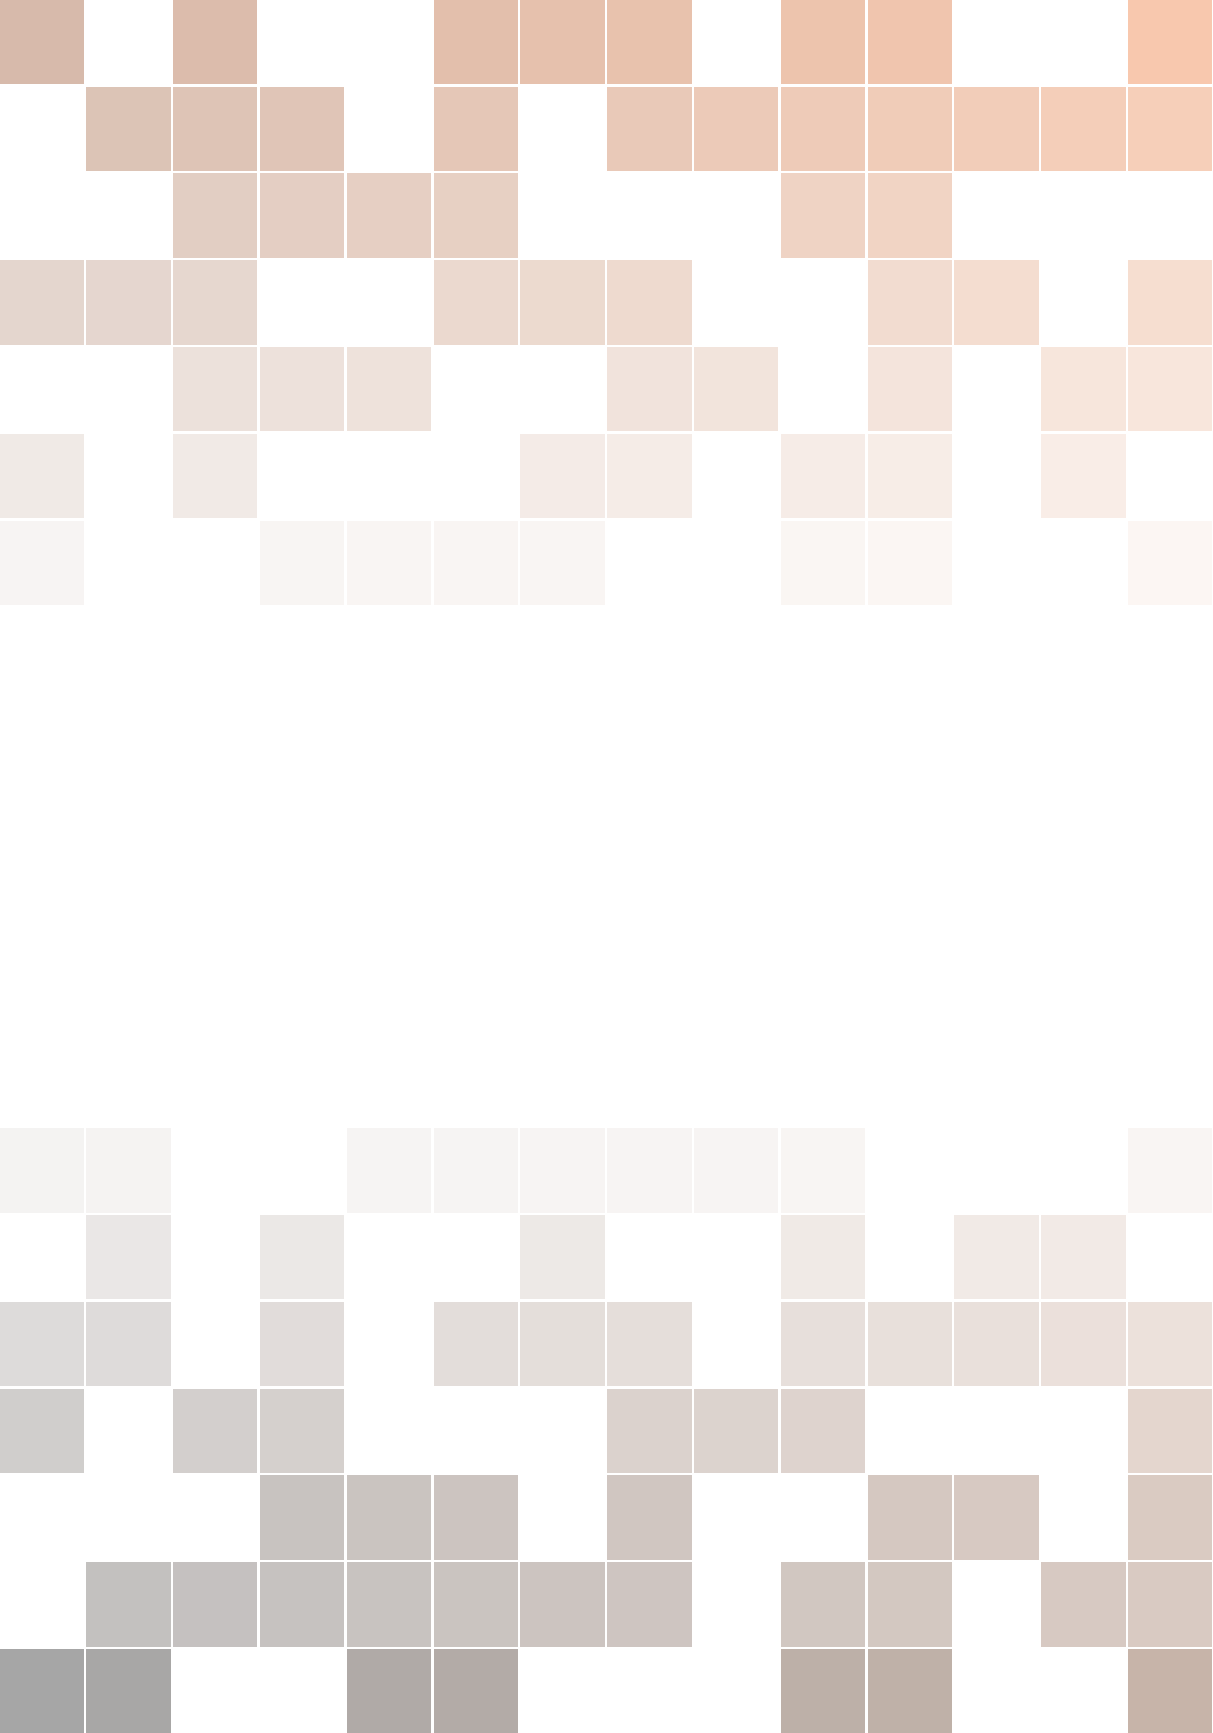
\includegraphics[scale=1]{background}}} % Image background
\par\normalfont\fontsize{15}{15}\sffamily\selectfont
“OpenQuake: Calculate, share, explore”
\centering
\vspace*{9cm}
\par\normalfont\fontsize{35}{35}\sffamily\selectfont
Ground Motion Prediction Equation (GMPE) and Strong Motion Modeller's Tookit - User Guide\par % Book title
\endgroup

%----------------------------------------------------------------------------------------
%	COPYRIGHT PAGE
%----------------------------------------------------------------------------------------

\newpage
~\vfill
\thispagestyle{empty}

\noindent Copyright \copyright\ 2014 GEM Foundation\\ % Copyright notice

\noindent \textsc{Published by GEM Foundation}\\ % Publisher

\noindent \textsc{globalquakemodel.org/openquake}\\ % URL

\noindent 
   {\bf{Disclaimer}} \hfill \\
   The ``Ground Motion Prediction Equation (GMPE) and Strong Motion Modeller's Tookit - User Guide'' is distributed in the hope that it will be useful, but without any warranty: without 
   even the implied warranty of merchantability or fitness for a 
   particular purpose. While every 
   precaution has been taken in the preparation of this document, in 
   no event shall the authors of the manual and the GEM Foundation be 
   liable to any party for direct, indirect, special, incidental, or 
   consequential damages, including lost profits, arising out of the 
   use of information contained in this document or from the use of 
   programs and source code that may accompany it, even if the authors 
   and GEM Foundation have been advised of the possibility of such damage. 
   The Book provided hereunder is on as "as is" basis, and the authors 
   and GEM Foundation have no obligations to provide maintenance, support,
   updates, enhancements, or modifications. 
   \hfill \\
   \todo{This needs to be updated or removed}
   The current version of the book has been revised only by members of 
   the GEM model facility and it must be considered a draft copy. 
   %
   \vspace{0.4cm} \hfill \\
   {\bf{License}} \hfill \\
   This Book is distributed under the Creative Common License 
   Attribution-NonCommercial-NoDerivs 3.0 Unported (CC BY-NC-ND 3.0) 
   (see link below). You can download this Book and share it with 
   others as long as you provide proper credit, but you cannot change 
   it in any way or use it commercially. 
   \hfill \\

\noindent \textit{First printing, June 2014} % Printing/edition date

%----------------------------------------------------------------------------------------
%	TABLE OF CONTENTS
%----------------------------------------------------------------------------------------

\chapterimage{./figures/chapter_head_1.pdf} % Table of contents heading image

\pagestyle{empty} % No headers

\tableofcontents % Print the table of contents itself

\cleardoublepage % Forces the first chapter to start on an odd page so it's on the right

\pagestyle{fancy} % Print headers again

%----------------------------------------------------------------------------------------
%	CHAPTER 1
%----------------------------------------------------------------------------------------
\chapterimage{./figures/chapter_head_2.pdf} % Chapter heading image
\chapter{Introduction}
\label{chap:intro}
\section{A Ground Motion Prediction Equation (GMPE) Toolkit}
\label{sec:gmpe_toolkit}

Probabilistic Seismic Hazard Assessment (PSHA) is well-established as a robust and effective means of characterising the level of ground shaking to which a structure may be subject within a given time period. Since its inception in the 1960s the PSHA methodology undergone many developments designed to improve the characterisation of the physical properties of the rupture source, the ground motion attenuation and the site amplification. Often leading these developments are the Ground Motion Prediction Equations (GMPEs), which characterise the manner in which ground motion measures (intensity measures) vary with the source, path and site properties of observed ground motion records. 

The widespread adoption of PSHA for site-specific, urban-level and national/regional-scale analyses of earthquake hazard has created a clear need for calculation software to be widely available for this purpose. Furthermore, in recent years that has been an increasing need for PSHA calculation software to be widely available, for its processes to be open, and for a commitment to quality assurance. Recognising this need the Global Earthquake Model (GEM) Foundation created OpenQuake, an open-source software for calculation of probabilistic seismic hazard and risk, that is developed using a test-driven philosophy in which the software undergoes extensive testing and quality assurance as part of the construction process. 

Whilst OpenQuake itself is designed to fullfill the need for open and tested software for PSHA calculation, it does not explicitly address the issue of PSHA model construction. A PSHA model can be broken down into three components: the seismogenic source model(s), the ground motion prediction equations and the logic tree to characterise the model-to-model uncertainty in an equation. GEM is now in the process of endeavouring to extend the OpenQuake development approach to the area of PSHA model construction. It has done so with the development of two ``Modeller's Toolkit's: 

\begin{enumerate}
\item \textbf{The Hazard Modeller's Toolkit} , a suite of open-source tools for the preparation of seismogenic source models for application in PSHA \cite{hmtk_guide}
\item \textbf{The OpenQuake Ground Motion Toolkit}, a suite of open-source tools for analysis and interpretation of observed ground motions and ground motion prediction equations, for the purposes of GMPE selection in PSHA (this document)
\end{enumerate}

This document presents the OpenQuake Ground Motion Toolkit, or GMPE-SMTK hereafter, providing an overview of the features as well as practical examples that demonstrate how to use the toolkit in real applications. 

\section{Objectives and Structure}
\label{sec:objectives}

The GMPE-SMTK serves the primary objective of assisting seismic hazard modellers with the process of understanding and identifying GMPEs for application in seismic hazard analysis. It brings together a collection of tools for visualising and exploring ground motion prediction equations, for analysing ground motion records to derive widely used ground motion intensity measures, and to compare observed ground motion intensity levels against the values predicted by the GMPE. To do this, however, the GMPE-SMTK has needed to create an internal data structure to store and process databases of ground motion records. A general overview of the GMPE-SMTK is shown in Figure \ref{fig:smtk_overview}.

\begin{figure}[htb]
	\centering
		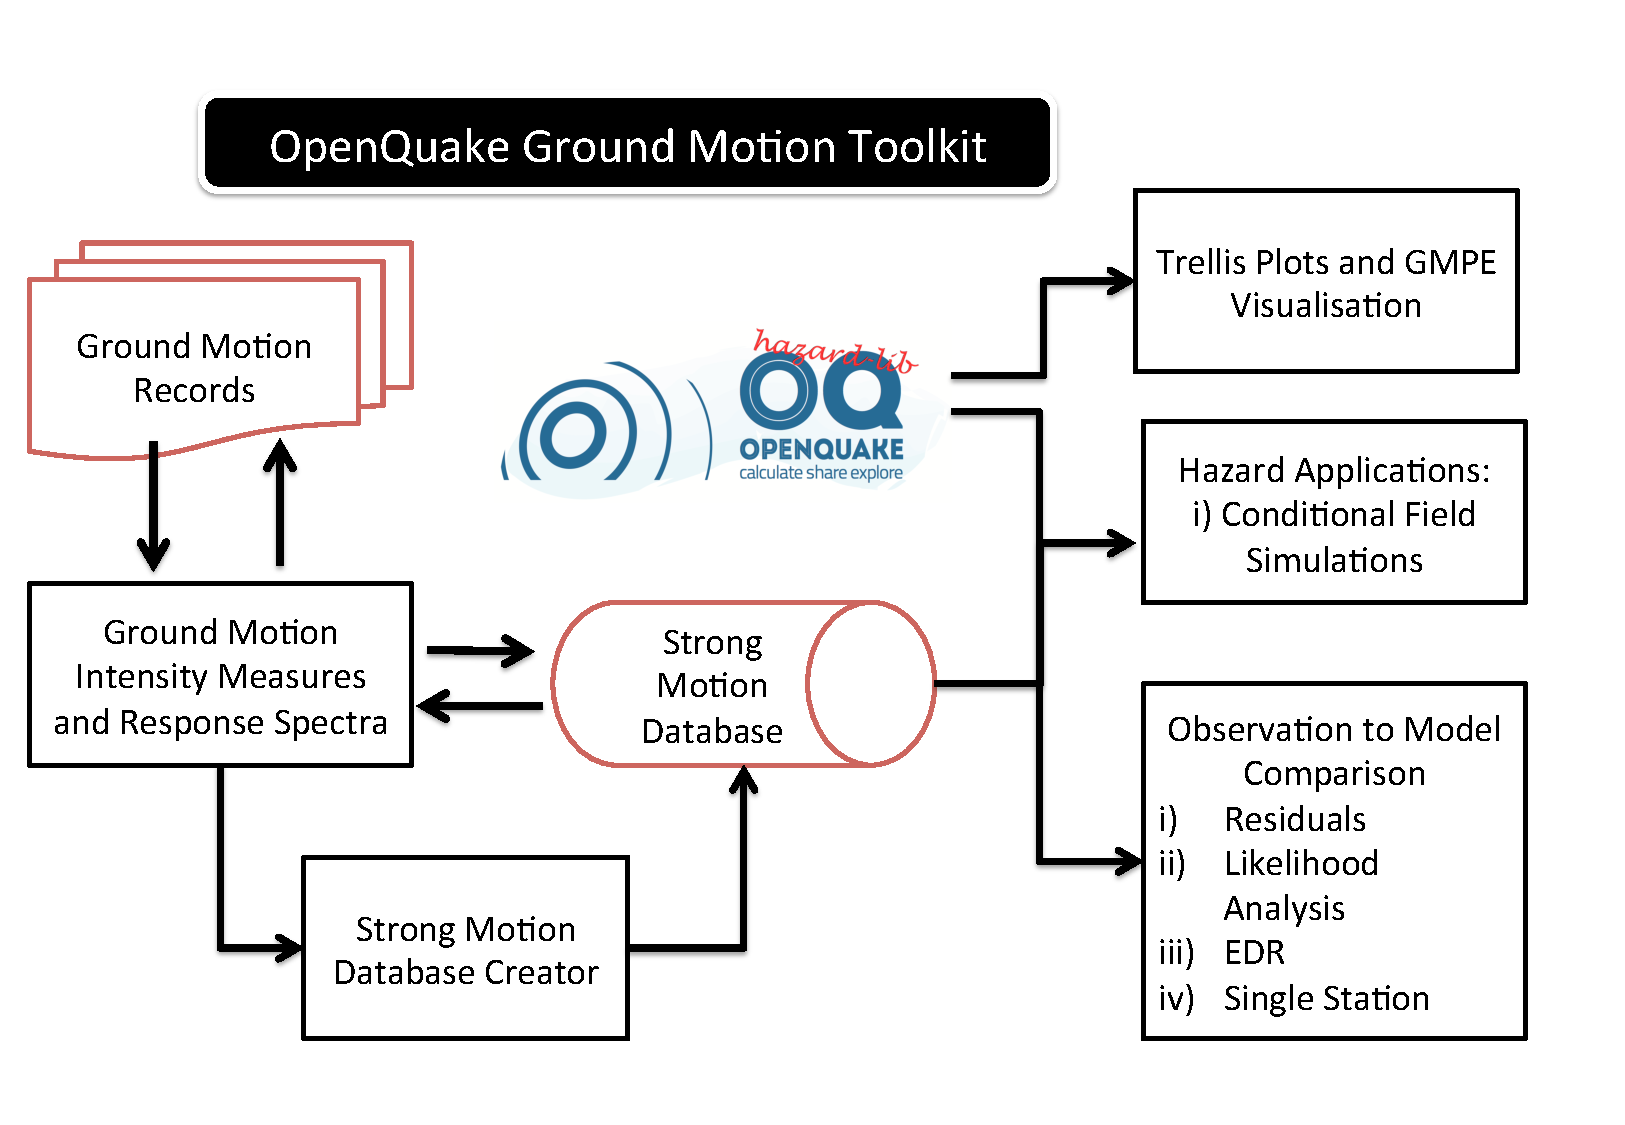
\includegraphics[width=\textwidth]{./figures/intro/smtk_architecture_flowchart.pdf}
	\caption{Feature Overview of the OpenQuake Ground Motion Toolkit}
	\label{fig:smtk_overview}
\end{figure}

The critical element within this process is the usage of OpenQuake, or more specifically the OpenQuake Hazard Library, as a dependency within the toolkit. It is from this library that we take the GMPEs, as well as various tools for undertaking calculations of source to site geometry. By using OpenQuake's own library we inherit OpenQuake's testing and quality assurance process for implementation of GMPEs. We also ensure total consistency between the GMPEs used for comparison against strong motion records and those used within the OpenQuake PSHA calculation engine itself. This is a feature that is unique to this toolkit. 

A list of the current functionalities is given in Table \ref{tab:features}.

\begin{table}
\centering
\begin{tabular}{|c|c|} \hline
\textbf{Feature} & \textbf{Algorithm} \\ \hline
Ground Motion  &  Retrieve PGA, PGV and PGD \\
Intensity Measures  &  Response Spectra - Newmark-$\beta$ \\
  &   Response Spectra - \cite{NigamJennings1969} \\
  &   Horizontal Spectra (Geometric Mean, Envelope etc.) \\
  &   Rotate Horizontal Record Pairs \\
  &   Rotational Spectra (GMRotD, GMRotI) \cite{Boore_etal2006} \\ \hline
Trellis Plotting & Configure Rupture \\
                 & Compare GMPE Scaling with Magnitude \\
                 & Compare GMPE Scaling with Distance \\
                 & Compare GMPE Spectra with Magnitude \& Distance \\ \hline
Comparison with  & Get GMPE residuals from Ground Motion ... \\
Observations     & ... measure residual distribution \\
                 & ... retrieve inter- and intra-event residual \\
                 & ... view trends with magnitude \\
                 & ... view trends with distance \\
                 & ... view trends with $V_{S30}$ \\
                 & ... view trends with event depth \\
                 & Likelihood Analysis \cite{Scherbaum_etal2004}\\
                 & Log-likeihood Analysis \cite{Scherbaum_etal2009}\\
                 & Euclidean Distance-Based Ranking \cite{KaleAkkar2013}\\
                 & Single-Site Residual Analysis \\ \hline
Hazard Applications & Conditional Field Simulation \\ \hline
\end{tabular}
\caption{Current features within the OpenQuake Ground Motion Toolkit}
\label{tab:features}

\end{table}

\section{Installation and Getting Started}
\label{sec:installation}

The software is available on the open Github repository: \href{https://github.com/g-weatherill/gmpe-smtk}{https://github.com/g-weatherill/gmpe-smtk}. Installation is dependent on the OpenQuake hazardlib and nrmllib libraries. These can be retrieve from the following repositories:
\begin{itemize}
\item OpenQuake Hazard Library (oq-hazardlib)\\
\href{https://github.com/gem/oq-hazardlib}{https://github.com/gem/oq-hazardlib}
\item OpenQuake Natural Risk Markup Language (NRML) Library (oq-nrmllib)\\
\href{https://github.com/gem/oq-nrmllib}{https://github.com/gem/oq-nrmllib}
\end{itemize}

The GMPE-SMTK has the following dependencies:

\begin{itemize}
\item \textbf{Numpy 1.6.1 or later}
\item \textbf{Scipy 0.11.0 or later}
\item \textbf{Matplotlib 1.3.x or later}
\item \textbf{H5py 2.2.0 or later}
\item \textbf{lxml}
\item \textbf{Shapely 1.2.18 or later}
\item \textbf{oq-hazardlib (brings in Numpy, Scipy and Shapely)}
\item \textbf{oq-nrmllib (brings in lxml\footnote{Except on Windows})} 
\end{itemize}


\subsection{Windows}

For a comprehensive Python installation including many of the dependencies needed to both the toolkit and the OpenQuake libraries the best option is a full installation of PythonXY. This software is freely available from here: \href{https://code.google.com/p/pythonxy/}{https://code.google.com/p/pythonxy/}. It is recommended to proceed with a \emph{full} installation and ensure that all of the above dependencies are selected for installation where available.

For the oq-nrmllib it is necessary to install the Lxml library (\href{http://lxml.de}{http://lxml.de}). This is not officially supported for Windows, so it is recommended (by Python developers themselves!) to install the unofficial Lxml binding from here: \footnote{\href{http://www.lfd.uci.edu/~gohlke/pythonlibs/}{http://www.lfd.uci.edu/~gohlke/pythonlibs/}}. Download and then run the 32-bit package named ``lxml-\#.\#.\#.win32-py2.7.exe''.

Next you will need to install the op-hazardlib and oq-nrmllib. From the web repositories listed previously click the button ``Download Zip'', then extract contents to the folders \verb=C:/oq-hazardlib= and \verb=C:/oq-nrmllib= respectively.

Open an enhanced IPython console. Go to Start $->$ Python(xy) $->$ Enhanced Consoles $->$ Ipython (sh). This will open up an Ipython console terminal. To install the oq-hazardlib, at the console prompt type:

\begin{Verbatim}[frame=single, commandchars=\\\{\}, fontsize=\scriptsize]
~$: cd C:/oq-hazardlib/
~$: python setup.py install build --compiler=mingw32
\end{Verbatim}

This will install the oq-hazardlib with the full C-extensions, which speed up some of the geometry calculations. Then do the same with the oq-nrmllib.

\begin{Verbatim}[frame=single, commandchars=\\\{\}, fontsize=\scriptsize]
~$: cd C:/oq-hazardlib/
~$: python setup.py install
\end{Verbatim}

Then close the console by typing \verb=exit=. 

Finally, download the zipped folder of the GMPE-SMTK from the github repository and unzip to a folder of your choosing. To allow for usage of the GMPE-SMTK throughout your operating system, do the following: 

\begin{enumerate}
\item From the desktop, right-click \textbf{My Computer} and open \textbf{Properties}
\item In the ``System Properties'' window click on the \textbf{Advanced} tab.
\item From the ``Advanced'' section open the \textbf{Environment Variables}.
\item In the ``Environment Variables'' you sill see a list of ``System Variables'', select ``Path'' and ``Edit''.
\item Add the path to the hmtk directory to the list of folders then save.
\end{enumerate}

After this process it may be necessary to restart PythonXY.

\subsection{OSX and Linux}

For installation on unix platforms we recommend installing each package using the Python Package manager (Pip). Assuming that Python 2.7.3 is already installed on your system, the Package Manager can be installed using the command line:

\begin{verbatim}
~$ python get-pip.py 
\end{verbatim}

First it is recommended to install the OpenQuake libraries (as they bring in most of the dependencies!). These can be done using Git to clone the repositories:

\begin{verbatim}
# Clone the hazardlib repository
git clone https://github.com/gem/oq-hazardlib.git
cd oq-hazardlib
# Run the installation
sudo python setup.py install
cd ..
# Clone the nrmllib repository
git clone https://github.com/gem/oq-nrmllib.git
cd oq-nrmllib
sudo python setup.py install
\end{verbatim}

Then use PiP to install Matplotlib and H5py:

\begin{verbatim}
# Install Matplotlib
sudo pip install matplotlib
# Install H5py
sudo pip install h5py
\end{verbatim}

Finally all that is needed is to install the GMPE-SMTK. As with the OpenQuake libraries the best option is to use Git to clone the repository:

\begin{verbatim}
# Clone the repository
~$ git clone https://github.com/g-weatherill/gmpe-smtk.git
\end{verbatim}

As the repository does not have an installer the directory should be added manually to the Pythonpath. This can be done from the bash profile script using a suitable text editor (Vim in the example below):

\begin{verbatim}
# Open the profile script
~$ vim ~/.profile
# Add the following line to the bottom of the profile script
export PYTHONPATH=/Users/GW/Documents/GEM/hmtk/gmpe-smtk/:$PYTHONPATH
# Save and exit
\end{verbatim}

To complete the installation simply re-start the terminal.










%----------------------------------------------------------------------------------------
%	CHAPTER 2
%----------------------------------------------------------------------------------------
\chapterimage{./figures/chapter_head_2.pdf} % Chapter heading image
\chapter{The Ground Motion Database}
\label{chap:database}
\section{Strong Motion Observations}
\label{sec:data_model}

The core structure of the GMPE-SMTK is based upon defining a reference model for describing a database of ground motion data. This means that inside of the software every database is rendered into a common, but potentially extensible, format in which the difference components of the information pertaining to a particular ground motion record is structured in a logical and readily interpretable manner. The initial structure of the ``data model'' is constructed to permit a widely applicable, but not exhaustive, representation of the set of attributes to describe the characteristics of the strong motion record. 

\section{Current Data Model}

The comprehensive data model is shown in Figure \ref{fig:sm_data_model}. It's two core classes are the strong motion database (recognised internally in the toolkit as \verb=smtk.sm_database.GroundMotionDatabase=) and the ground motion record (\verb=smtk.sm_database.GroundMotionRecord=). The database itself only contains four attributes:

\begin{itemize}
\item \verb=id=: The unique identifier of the database
\item \verb=name=: The database name
\item \verb=directory=: The location of the directory containing the database files
\item \verb=records=: The ground motion records as a list of instances of\\\verb=smtk.sm_database.GroundMotionRecord=
\end{itemize}

The class also contains the method \verb=get_contexts=. This method is fundamental to the operation of the toolkit as it translates the database into the form required for input into the OpenQuake Ground Motion Prediction Equations. To calculate the expected ground motions, using a GMPE, given the input information OpenQuake requires a set of ``context'' objects: \verb=SitesContext=, \verb=DistancesContext= and \verb=RuptureContext=. These are a set of containers that hold information needed for OpenQuakes's GMPE's\footnote{Their contents will generally reflect the full list of parameters needed for all of the GMPEs currently implemented in OpenQuake. Depending on the GMPEs being considered, however, not all parameters need to be included.}. The ``contexts'' operate such that a single rupture can be associated with a set of sites and distances. Therefore when creating the contexts the \verb=get_contexts= functoin will group records according to the earthquake ID and produce a set of context objects per event, not per record. \textbf{It is absolutely critical for correct usage of the toolkit that the event IDs are correctly, and uniquely (i.e. a strong record can only be associated to one event) assigned for each record.}

\begin{figure}[htb]
	\centering
		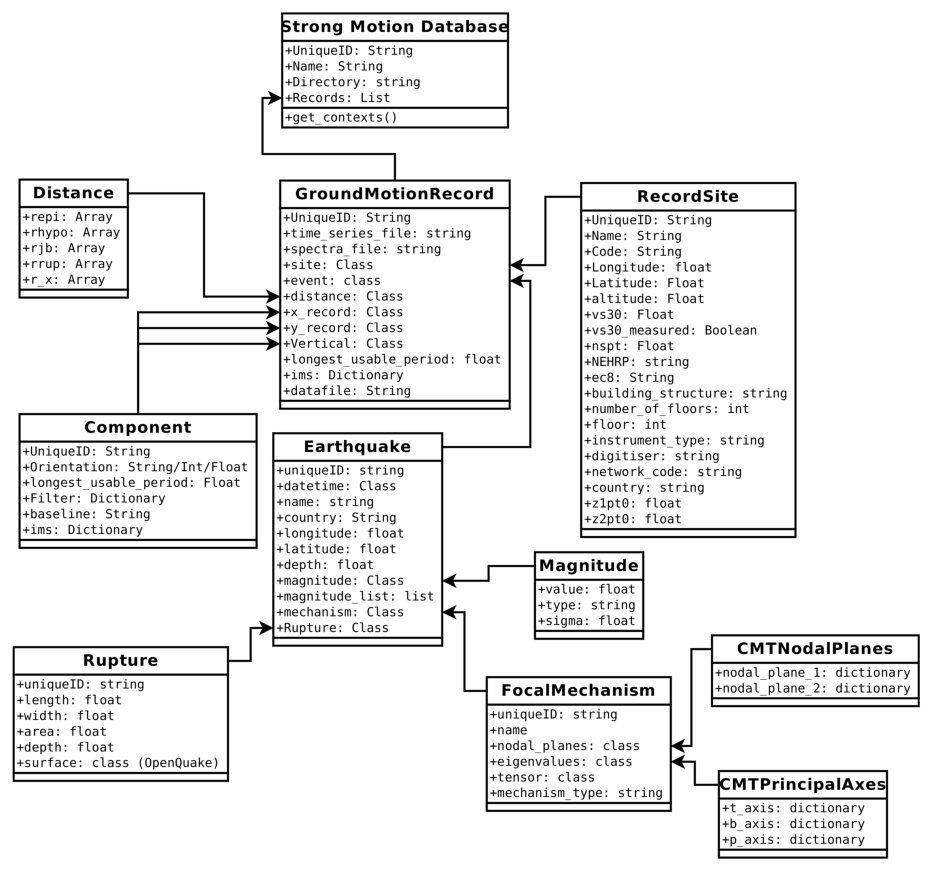
\includegraphics[width=\textwidth]{./figures/database/sm_database_attributes.pdf}
	\caption{Core Architecture of the Strong Motion Data Model}
	\label{fig:sm_data_model}
\end{figure}

The \verb=GroundMotionRecord= class is largely a single container of attributes:
\begin{itemize}
\item \verb=id= Record (waveform) ID
\item \verb=time_series_file=: List of names of the files storing the time series of each of the components of the record.
\item \verb=spectra_file=: List of names of the files storing the response spectra of each of the components of the record (Optional).
\item \verb=event=: Earthquake information as an instance of the \verb=Earthquake= class
\item \verb=distance=: Source to site distance information as an instance of the \verb=RecordDistance= class
\item \verb=site=: Site information as an instance of the \verb=RecordSite= class.
\item \verb=xrecord=: Metadata relating to the first horizontal component of the record as an instance of the class \verb=Component=
\item \verb=yrecord=: Metadata relating to the second horizontal component of the record as an instance of the class \verb=Component=
\item \verb=vertical=: Metadata relating to the vertical component of the record as an instance of the class \verb=Component= (Optional)
\item \verb=average_lup=: Average longest useable period of the record
\item \verb=ims=: Dictionary of scalar intensity measure attributes of the record
\item \verb=datafile=: Location of the processed hdf5 database file for the record.
\end{itemize}


\subsection{Source Characteristics}

The current characterisation of the source is broken down into several different areas: the hypocentre information, magnitude, focal mechanism and finite rupture.

\subsubsection{Earthquake}

The \verb=Earthquake= class contains full characterisation of the event source, with the following attributes:

\begin{itemize}
\item \verb=id=: Unique identifier of the event
\item \verb=datetime=: The date and time of the earthquake as an instance of Python's datetime object. This can be generated as follows:
\begin{python}
from datetime import datetime
# The following event occurs at 2010/6/1 20:36:27.4
event_date_time = datetime(2010, 6, 1, 20, 36, 27, 4E5)
\end{python}
\item \verb=name=: Event Name
\item \verb=country=: Country of event (Optional)
\item \verb=longitude=: Longitude of event (in decimal degrees)
\item \verb=latitude=: Latitude of event (in decimal degrees)
\item \verb=depth=: Hypocentral depth of event (km)
\item \verb=magnitude=: Primary magnitude (usually $M_W$) as instance of the \verb=Magnitude= class
\item \verb=magnitude_list=: Alternative magnitudes for the event, as list of instances of the \verb=Magnitude= class
\item \verb=mechanism=: Earthquake focal mechanism as instance of the \verb=FocalMechanism= class
\item \verb=rupture=: Finite rupture properties as instance of the \verb=Rupture= class
\end{itemize}

In general the preferred magnitude scale is Moment Magnitude $M_W$; however to permit the possibility other scales may be preferred (or for practical purposes assumed equivalent) the \verb=Earthquake= class contains the primary magnitude and a list of other magnitude scales. A magnitude is represented by a separate class called \verb=Magnitude=, which contains the following attributes:

\begin{itemize}
\item \verb=value= The magnitude value
\item \verb=mtype= The magnitude type
\item \verb=sigma= The standard deviation of the magnitude estimate
\end{itemize}

Where possible it is preferable to hold information relating to the focal mechanism of the class. It is anticipated that potentially several components of the focal mechanism may be needed; hence the mechanism is broken down into classes to represent the nodal planes, the eigendecomposition and the moment tensor, all held within the \verb=FocalMechanism= class. This class has the following attributes:
\begin{itemize}
\item \verb=id= Unique identifier (should be different from the event ID)
\item \verb=Name= Focal mechanism name
\item \verb=nodal_planes= The strike dip and rake of the two nodal planes of the focal mechanism as an instance of the class \verb=GCMTNodalPlanes=. This class can be constructed as follows:
\begin{python}
# Two nodal planes: i) Strike = 30., dip = 90., rake = 0.
#                  ii) Strike = 120., dip = 90., rake = 180.
from smtk.sm_database import GCMTNodalPlanes
nps = GCMTNodalPlanes
nps.nodal_plane_1 = {"strike": 30., "dip": 90., "rake" = 0.}
nps.nodal_plane_2 = {"strike": 120., "dip": 90., "rake" = 180.}
\end{python}
 \item \verb=eigenvalues= The eigenvectors (B-, P- and T-) of the principal axes of the mechanism as an instance of the class \verb=GMCTPrincipalAxes=. This can be constructed as follows:
 \begin{python}[frame=single]
 # Mechanism with the following planes
 # T-axis = Eigenvalue 1.5E24, Plunge = 8, Azimuth = 203
 # B-axis = Eigenvalue -0.11E24, Plunge = 77, Azimuth = 332
 # P-axis = Eigenvalue -1.393, Plunge = 10, Azimuth = 111
 from smtk.sm_database import GCMTPrincipalAxes
 pax1 = GCMTPrincipalAxes()
 pax1.t_axis = {"eigenvalue": 1.5E24,
                "azimuth": 203.,
                "plunge": 8.}
 pax1.b_axis = {"eigenvalue": -0.11E24,
                "azimuth": 332.,
                "plunge": 77.}
 pax1.p_axis = {"eigenvalue": -1.393E24,
                "azimuth": 111.,
                "plunge": 10.}
 \end{python}
 \item \verb=tensor= The moment tensor as a $3 \times $ array
 \item \verb=mechanism_type= The style of faulting as a string
\end{itemize}

Finally the \verb=Earthquake= class can contain information relating to the physical dimensions of the rupture (where available!). These are held in the \verb=Rupture= class, with the following attributes:
\begin{itemize}
\item \verb=id=: Unique ID (not the same as the event ID)
\item \verb=length=: Rupture length (km)
\item \verb=width=: Rupture Width (km)
\item \verb=area=: Rupture Area (km$^2$)
\item \verb=depth=: Depth to the top of rupture (km)
\item \verb=surface=: Rupture surface as an instance of the OpenQuake surface class
\end{itemize}


\subsection{Site Characteristics}

In contrast to the \verb=Earthquake= class, all relevant site information is stored in just one class: \verb=RecordSite=. This class contains the following attributes:
\begin{itemize}
\item \verb=id=: Unique station identifier
\item \verb=name=: Station Name
\item \verb=code=: Station Code (as reported by station)
\item \verb=longitude=: Longitude of station
\item \verb=latitude=: Latitude of station
\item \verb=altitude=: Elevation of station (optional)
\item \verb=vs30=: $V_{S30}$ of station
\item \verb=vs30_measured=: Boolean term to indicate if the $V_{S30}$ is measure (True) or inferred (False) (optional)
\item \verb=vs30_measured_type=: Metadata indicating how $V_{S30}$ is measured (optional)
\item \verb=nspt=: Number of hammer blows from standard penetration test (optional)
\item \verb=nehrp=: NEHRP site class (optional)
\item \verb=ec8=: Eurocode 8 site class (optional)
\item \verb=building_structure=: Type of building hosting the recorder (optional)
\item \verb=number_floors=: Number of floors in building hosting the recorder (optional)
\item \verb=floor=: Floor upon which the recorder is situated (optional)
\item \verb=instrument_type=: Type of recording instrument
\item \verb=digitiser=: Type of digitiser
\item \verb=network_code=: Network code
\item \verb=country=: Country of station
\item \verb=z1pt0=: Depth to $V_S$ 1.0 km/s interface (m)
\item \verb=z2pt5=: Depth to $V_S$ 2.5 km/s interface (km)
\end{itemize}

\subsection{Waveform Characteristic}

The database can contain information relating to the manner in which the record has been processed, in addition to other waveform-specific metadata. This information is held in the \verb=Component= class, with the following attributes:
\begin{itemize}
\item \verb=id=: Identifier of the waveform
\item \verb=orientation=: Orientation of the record 
\item \verb=lup=: Longest useable period
\item \verb=filter=: Information about the filter type used. For example, for a ``Butterworth'' filter of 2nd order, with 2 passes and a high and low-cut frequency of 100 Hz and 0.05 Hz respectively, the filter is described via the dictionary:
\begin{python}[frame=single]
filter_data = {"Type": "Butterworth",
               "Order": 2,
               "Passes": 2,
               "Low-Cut": 0.05,
               "High-Cut": 100.0}
\end{python}
Additional data can be added dynamically where necessary
\item \verb=baseline=: Information about baseline adjustment
\item \verb=ims=: Scalar intensity measures of the component.
\item \verb=units=: Units of the waveform
\end{itemize}

\subsection{Geometry Characterisations}

Depending on the information supplied, particularly with respect to the finite rupture, the source-to-site geometry characteristics can be stored in the \verb=RecordDistance= class. In the present form this contains attributes of the five main distance types:

\begin{itemize}
\item \verb=repi=: Epicentral distance (km) from source to site
\item \verb=rhypo=: Hypocentral distance (km)
\item \verb=rjb=: Joyner-Boore distance (km)
\item \verb=rrup=: Rupture distance (km)
\item \verb=r_x=: $R_X$ distance (km)
\end{itemize}

\section{Missing Metadata!}
\label{sec:missing_metadata}

One of the greatest challenges in construction of a strong motion database is to address the cases where critical (i.e. non-optional) metadata are missing from the record. 

\textbf{TODO - More to add!}

\section{The HDF5 Strong Motion Database}
\label{sec:hdf5}

The potentially widespread application of the software requires that the manner in which it is able to create and access waveform data is important to the practical function of the tools. Therefore the decision is made to store the waveforms and related attributes in an \verb=hdf5= database \footnote{\href{http://www.hdfgroup.org/HDF5/}{http://www.hdfgroup.org/HDF5/}}. \verb=hdf5= is a high density binary file format capable of storing data in a nested architecture, allowing large arrays of data (such as waveforms) to be mapped alongside their attributed This database consists of two components. The metadata for each record, mapped according to the \verb=GroundMotionDatabase= class, and the waveform data itself. The waveform data for a database is split into a directory of \verb=hdf5= 
binary files, where each file contains the full waveforms for all three components of the record, as well as the spectra for each waveform, and potentially the horizontally resolved spectra. The full structure of a single ground motion record in a binary format is shown in Figure \ref{fig:sm_hdf5_model}.

\begin{sidewaysfigure}[htbp]
	\centering
		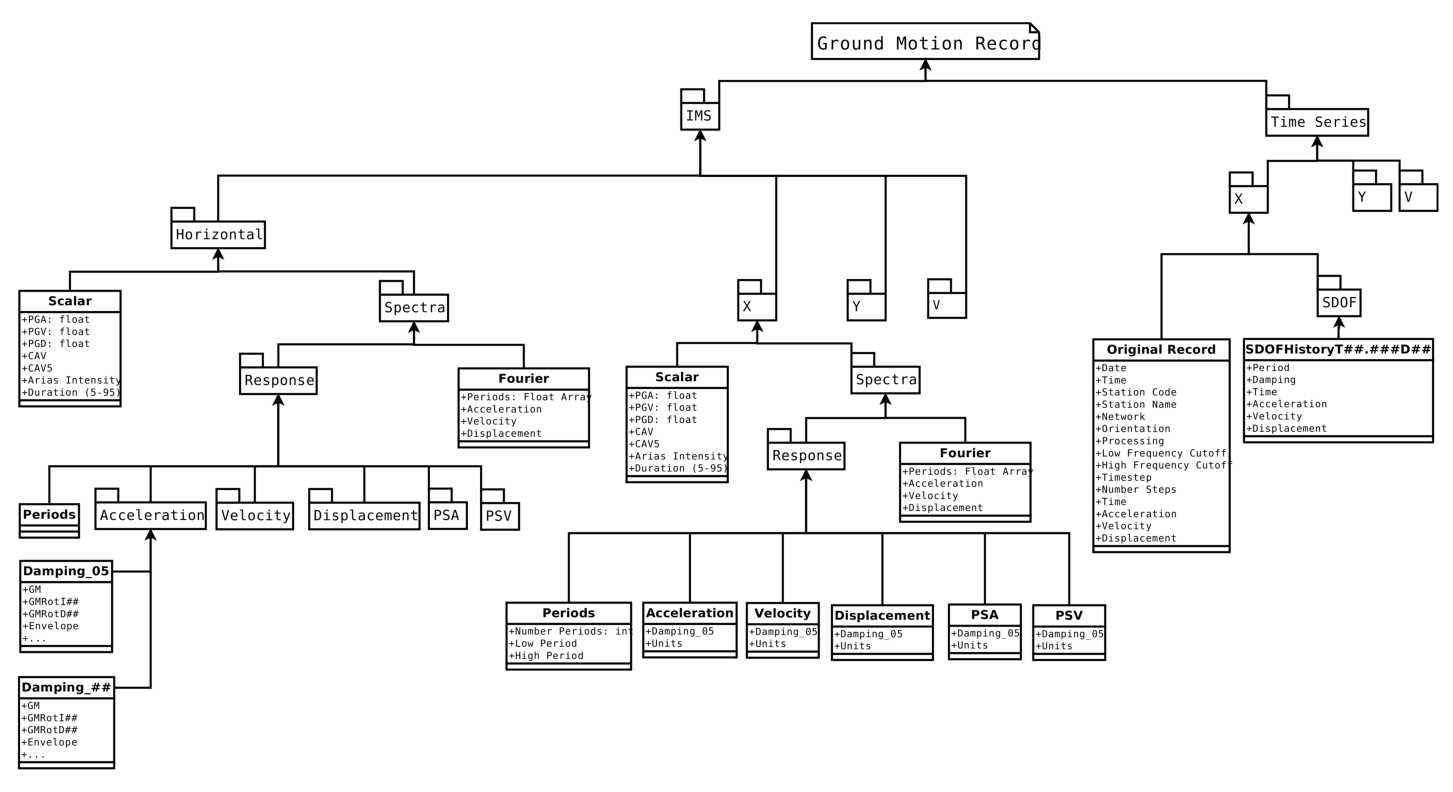
\includegraphics[width=\textwidth]{./figures/database/sm_database_architecture.pdf}
	\caption{Architecture of the hdf5 representation of a strong motion record}
	\label{fig:sm_hdf5_model}
\end{sidewaysfigure}

The \verb=hdf5= format offers several key advantages that have motivated its usage within these tools. Already mentioned was the capability to store large arrays of numerical data in a structure that is conveniently nested in order to associate subsets of data and corresponding attributes. The format is high-density, reducing the overall size of the datafile compared to, for example, plain text ascii format. The file structure is also dynamic allowing for attributes and dataset to be added as needed. This enables the user to undertake the data compilation in several steps, adding on processed data subsequently from the initial compilation stage. The \verb=hdf5= format is widely supported by many different software languages, and its contents visualisable via the cross-platform \verb=HDFView= application \footnote{\href{http://www.hdfgroup.org/products/java/hdfview/}{http://www.hdfgroup.org/products/java/hdfview/}}. 

\subsection{Loading Data to the Database}

In general the creation of a database from a set of records is a process that cannot be readily generalised as each strong motion recording network will define its own data format. Whilst progress is ongoing to add database creators for some of the largest strong motion recording networks, it is necessary for the user to create a customised reader for their own networks. The readers constitute a set of three separate modules, the outline of which can be found in the \verb=smtk.parsers.base_database_parser= module: i) \verb=SMDatabaseReader= the main reader to build the metadata structure of the database (i.e. the \verb=GroundMotionDatabase= class), ii) \verb=SMTimeSeriesReader= to read the waveforms from the respective time series files, and iii) \verb=SMSpectraReader= to read the spectra from files (if provided by the network). If the corresponding database creators are available then a full database can be created using the module \verb=smtk.sm_database_builder.SMDatabaseBuilder=, using the example below:

\begin{python}[frame=single]
# Import the readers for database XXXXX
from smtk.parsers.XXX_database_parser import (XXXMetadataReader,
                                              XXXTimeSeriesReader,
                                              XXXSpectraReader)
# Import the database builder
from smtk.sm_database_builder import SMDatabaseBuilder,

# Path to the directory containing the input files
input_fileset = "./path/to/strong/motion/folder"
# Path to the directory intended for the database
output_database = "./path/to/output/database/folder"

# Create an instance of the database builder
db_builder = SMDatabaseBuilder(XXXMetadataReader,
                               output_database)

# Create the metadata database
db_builder.build_database("UNIQUEID",  # Database ID
                          "DATABASE NAME",  # Name
                          input_fileset)

# Parse the strong motion records
db_builder.parse_records(XXXTimeSeriesReader,
                         XXXSpectraReader)

# (This may take some time if there are many records!!!)
\end{python}
%# If you wish to calculate the resultant horizontal ground motions (e.g. Geometric mean, GMRot etc.)
%# then you can add on this function

%from smtk.sm_database_builder import add_horizontal_im

%intensity_measures = ["PGA", "PGV", "Geometric", "GMRotD50", "GMRotI50"]
%add_horizontal_im(db_builder.database, intensity_measures, component="Geometric", damping="05", periods=[])

The time taken to create the database will obviously depend on many factors, including the number of records and the sampling frequency of each record. For large databases however it could potentially take many hours!

When compiled the database will store the metadata in a file inside the database directory named ``\verb=metadata.pkl=''. This file is a Python binary file (called a ``Pickle'' file or ``pkl'') that stores the \verb=GroundMotionDatabase= class. To load this data into the workspace simply do the following:

\begin{python}[frame=single]
# Import the cPickle module
import cPickle
db1 = cPickle.load(open("path/to/database/metafile.pkl", "r"))
\end{python}


\section{Selecting Subsets of Records from the Database}
\label{sec:sm_selector}

For many of the GMPE tools that will be shown in the rest of this book there will be a frequent need to consider only subsets of the full database. To do this a set of selection tools are created to facilitate the database selection process. These tools can be found in the module \verb=smtk.strong_motion_selector.SMRecordSelector=. To select a subset of the database it is simply necessary to do the following:

\begin{python}[frame=single]
# Import the selector
from smtk.strong_motion_selector import SMRecordSelector
# Create an instance of the class for a specific database
selector = SMRecordSelector(db1)

# Select the 3rd, 6th and 17th record in the database
db2 = selector.select_records([2, 5, 16], as_db=True)
\end{python}

The keyword \verb=as_db= tells the function whether to return the selected records as a new instance of the \verb=GroundMotionDatabase= class. In most cases it is advisable to set this to true, otherwise it will return the selected records as a list of \verb=GroundMotionRecord= classes.

The \verb=SMRecordSelector= has the following selection methods
\begin{itemize}
\item \verb;select_from_record_id(self, record_id);\\

Selects a record according to its waveform ID.

\item \verb;select_from_event_id(self, event_id, as_db=False);\\

Returns a set of records from a common event defined by its \verb=event_id=.

\item \verb;select_within_time(self, start_time=None, end_time=None, as_db=False);\\

Selects records within a specific time window, defined as the interval between \verb=start_time= and \verb=end_time= (both Python datetime objects). For example:

\begin{python}
# Select records between 1990/01/01 and 2010/12/31
db2 = selector.select_within_time(datetime(1990, 1, 1),
                                  datetime(2010, 12, 31),
                                  as_db=True)
\end{python}

\item \verb;select_within_depths(self, upper_depth=None,;\\
\verb;    lower_depth=None, as_db=False);\\

Selects records corresponding to events within a specific depth range defined as the interval between \verb=upper_depth= (km) and \verb=lower_depth= (km). If not specified \verb=upper_depth= defaults to zero, and lower depth defaults to $\infty$. Records missing a hypocentral depth will not be selected, therefore setting both limits to \verb=None= will effectively filter these records out of the database.

\item \verb;select_within_magnitude(self, lower=None, upper=None, as_db=False);\\

Select records corresponding to events within a magnitude range, defined as the interval between \verb=lower= (defaults to $-\infty$ if not specified) and \verb=upper= (defaults to $\infty$ if not specified).

\item \verb;select_by_station_country(self, country, as_db=False);\\

Returns the records within a specific country (input as a string). For example, to select only observations recorded in Italy:

\begin{python}
db2 = selector.select_by_station_country("Italy",
                                         as_db=True)
\end{python}

\item \verb;.select_by_site_attribute(self, attribute, value, as_db=False);\\

Select records corresponding to a particular site attribute (according the attributes listed in the \verb=RecordSite= class). For example to select records only recorded at ``Free-Field'' stations:

\begin{python}
db2 = selector.select_by_site_attribute("building_structure", 
                                        "Free-Field",
                                        as_db=True)
\end{python}

\item \verb;select_within_vs30_range(self, lower_vs30, upper_vs30, as_db=False);\\

Select records within a given Vs30 range defined as the interval between \verb=lower_vs30= and \verb=upper_vs30=, which default to $-\infty$ and $\infty$ if not specified. As with the depth selection, setting both \verb=lower_vs30= and \verb=upper_vs30= to \verb=None= will remove records missing $V_{S30}$ values from the database. 

\item \verb;select_stations_within_distance(self, location, distance, as_db=False);\\

Selects records from stations within a distance (km) of a specified location. The location must be input as an instance of an OpenQuake ``Point'' class. For example, to select records within 200 km of $30^{\circ}$E and $40^{\circ}$N:

\begin{python}
from openquake.hazardlib.geo.point import Point
location = Point(30.0, 40.0)
db2 = selector.select_stations_within_distance(location,
                                               200.0,
                                               as_db=True)
\end{python}

\item \verb;select_stations_within_region(self, region, as_db=False);\\

Selects station inside of a specified region defined by a polygon. The polygon must be input as an instance of the OpenQuake Polygon class. For example, to select all ground motions recorded within a square bounded by $30^{\circ}$E to $40^{\circ}$E and $20^{\circ}$N to $40^{\circ}$N:

\begin{python}
from openquake.hazardlib.geo.point import Point
from openquake.hazardlib.geo.polygon import Polygon

region = Polygon([Point(30.0, 40.0),
                  Point(40.0, 40.0),
                  Point(40.0, 20.0),
                  Point(30.0, 20.0)])
db2 = selector.select_stations_within_region(region,
                                             as_db=True)
\end{python}

\item \verb;select_within_distance_range(self, distance_type, shortest, furthest,;\\
\verb;    alternative=False, as_db=False);\\
Select records based on a source to site distance range, with the distance type specified by \verb=distance_type=, within the interval \verb=shortest= (defaults to 0 if not specified) and \verb=furthest= (defaults to $\infty$ if not specified). Recognising the possibility that some distance metric may be missing it is possible to also specify a second metric and corresponding distance limits as a tuple via the
\verb=alternative= keyword. For example, select records within a Joyner-Boore distance of 5 km and 50 km, and, if Joyner-Boore distance is not specified select records within an epicentral distance of 10 km and 70 km.

\begin{python}
db2 = selector.select_within_distance_range(
    "rjb", 5.0, 50.0,
    alternative=("repi", 10.0, 70.0),
    as_db=True) 
\end{python}

\item \verb;select_mechanism_type(self, mechanism_type, as_db=False);\\
Select records based on a descriptive event mechanism type. For example, to select records from ``strike-slip'' events:

\begin{python}
db2 = selector.select_mechanism_type("strike-slip",
                                     as_db=True) 
\end{python}

\item \verb;select_event_country(self, country, as_db=False);\\

Select records corresponding to events whose epicentres occur within a specific country

\item \verb;select_epicentre_within_distance_from_point(self, location, distance,;\\
\verb;    as_db=False);\\

Selects records from earthquakes whose epicentres are within a distance of a point. The point must be input as an instance of the OpenQuake ``Point'' class.

\item \verb;select_epicentre_within_region(self, region, as_db=False);\\

Selects records from event inside the specified region. The region must be defined as an instance of the OpenQuake ``Polygon'' class.

\item \verb;select_longest_usable_period(self, lup, as_db=False);\\

Selects records with a longest usable period greater than or equal to \verb=lup= (in seconds)

\end{itemize}

  






%----------------------------------------------------------------------------------------
%	CHAPTER 3
%----------------------------------------------------------------------------------------
\chapterimage{./figures/chapter_head_1.pdf} % Chapter heading image
\chapter{Response Spectra and Intensity Measures}
\label{chap:ims}
\section{Ground Motion Waveforms}
\label{sec:ims}

Fundamental to the use of the GMPE-SMTK is the strong motion waveform. For the widest portability we adopt the simplest representation of the waveform in the toolkit, which requires only the acceleration and the time steps. As seen in the previous chapter, the strong motion database stores the acceleration, velocity and displacement trace. 

\textbf{The conventional units for acceleration, velocity and displacement waveforms in the GMPE-SMTK are ``cm/s/s'', ``cm/s'' and ``cm'' respectively.}

The GMPE-SMTK contains two tools for extracting basic information and common ground motion intensity measures from single waveforms, or from a horizontal pair of waveforms: \verb=intensity_measures= and \verb=response_spectrum=. To use them in an application we can import them as follows:

\begin{python}[frame=single]
import smtk.intensity_measures as ims
import smtk.response_spectrum as rsp
\end{python}

This will load two objects into the workspace \verb=ims= (the intensity measure tools) and \verb=rsp= (the response spectrum tools)

In most applications we assume it is the acceleration time series that is available. In the following example we consider a pair of strong motion records, where each record is represented by a simple ascii (text) file:\verb=sm_record_x.txt= and \verb=sm_record_y.txt=. The timestep of each record is 0.002 s.

\begin{python}[frame=single]
# Import the numpy tools
import numpy as np
# Load in the records
accel_x = np.genfromtxt("sm_record_x.txt")
accel_y = np.genfromtxt("sm_record_y.txt")
time_step = 0.002
\end{python}

Once loaded the user can retrieve the velocity and displacement time-series, calculated using double integration of the acceleration time series. A simple tool to do this is found in the \verb=ims= tools:

\begin{python}[frame=single]
vel_x, disp_x = ims.get_velocity_displacement(accel_x,
                                              time_step,
                                              units="cm/s/s") 
\end{python}

\noindent where \verb=units= is the units of the uploaded record. 

\noindent The first steps one might wish to take when analysing a strong motion record is to look at the waveforms. To do this we make use of the simple tool inside the response spectrum package called \verb=plot_time_series=.
This can be called as follows for the x=component of the pair:

\begin{python}[frame=single]
rsp.plot_time_series(accel_x,
                     time_step,
                     velocity=vel_x,
                     displacement=disp_x,
                     units="cm/s/s",
                     filename="path/to/output/image.eps",
                     filetype="eps",
                     dpi=300,
                     linewidth=1.5) 
\end{python}

This command would produce a plot of the style shown in Figure \ref{fig:time_series}.

\begin{figure}[htb]
	\centering
		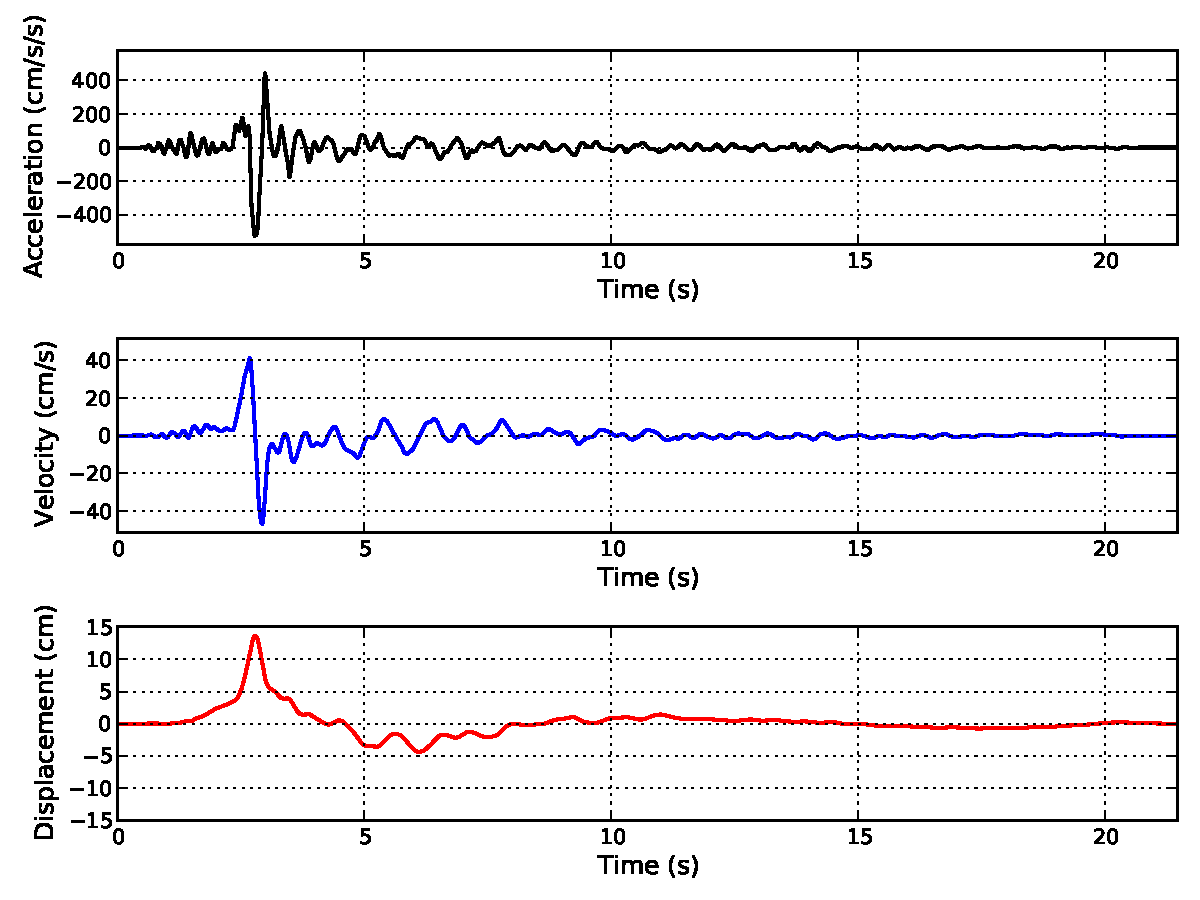
\includegraphics[height=8cm, keepaspectratio=true]{./figures/ims/timeseries_plot1.pdf}
	\caption{Example time series for a single record: acceleration (top), velocity (middle) and displacement (bottom)}
	\label{fig:time_series}
\end{figure}

\noindent The function \verb=plot_time_series= requires two essential arguments: 
\begin{itemize}
\item \verb=acceleration=: The acceleration time series
\item \verb=time_step=: The time step of the acceleration time series
\end{itemize}

\noindent If the user already has the velocity and displacement time series available these can be input with the following keyword arguments:

\begin{itemize}
\item \verb=velocity=: The velocity time series (cm/s), which will be calculated if not provided.
\item \verb=displacement=: The time step of the displacement (cm) time series, which will be calculated if not provided.
\item \verb=units=: The units of the acceleration time series (defaults to ``cm/s/s'')
\item \verb=figure_size=: The internal size of the figure (defaults to $(8, 6)$)
\item \verb=filename=: The name of the file to which the figure will be saved (if desired, by default it is ``None'')
\item \verb=filetype=: The format of the output file (default=``png'').
\item \verb=dpi=: Resolution (dots per inch) of the output figure (default = 300)
\item \verb=linewidth=: The thickness (point size) of the lines (default = 1.5)
\end{itemize}


\section{Scalar Intensity Measures}
\label{sec:scalar_ims}

\subsection{Peak Measures}

The following describes the simple ``peak'' measures, peak ground acceleration (PGA), peak ground velocity (PGV) and peak ground displacement (PGD), that can be extracted from the record:
\begin{align}
PGA = \max |a \left( t \right)| \nonumber\\
PGV = \max |v \left( t \right)| \\
PGD = \max |d \left( t \right)| \nonumber
\end{align}
where $a \left( t \right)$, $v \left( t \right)$ and $d \left( t \right)$ are the acceleration, velocity and displacement time series respectively.

These values can all be extracted by one function in the \verb=ims= tool named \verb=get_peak_measures=. These values can be called as follows:

\begin{python}[frame=single]
pga, pgv, pgd, vel_x, disp_x = get_peak_measures(time_step,
                                                 accel_x,
                                                 get_vel=True,
                                                 get_disp=True)
\end{python}

\noindent This function returns the three peak measures as well as the velocity and displacement (if required). The keywords \verb=get_vel= and \verb=get_disp= will, when set to \verb=True=, calculate velocity and displacement.

\subsection{Duration}
\subsection{Other Scalar Measures}

\section{Response Spectra}
\label{sec:response_spectra}

The response spectrum is one of the most important elements of a ground motion record used in earthquake engineering. The response spectrum provides the peak responses of a set a single-degree-of-freedom (SDOF) oscillators with different natural periods ($T$), and damping ratio $\xi$. The pseudospectral acceleration at a given period $Sa \left({T, \xi} \right)$, and its corresponding pseudospectral velocity and displacements, $Sv \left( {T, \xi} \right)$ and $Sd \left( {T, \xi} \right)$ respectively, are the most widely used means to characterise the ground motion input for a given structure. In addition to the peak values however, it is also useful to have available the acceleration, velocity and displacement response time series of the SDOF oscillators for each natural period. The GMPE-SMTK response spectra tools are designed to return the most comprehensive set of information to describe the SDOF response for each record.

To calculate a response spectrum for a record, two response spectra calculators are currently available: ``Newmark-$\beta$'' and ``Nigam \& Jennings'' (CITE NigamJennings1969).

These can be called following the process below:
\begin{python}
# Define the periods for calculating spectral acceleration
periods = np.array([0.01, 0.02, 0.03, 0.04, 0.05, 0.075, 0.1, 
                    0.11, 0.12, 0.13, 0.14, 0.15, 0.16, 0.17, 
                    0.18, 0.19, 0.20, 0.22, 0.24, 0.26, 0.28,
                    0.30, 0.32, 0.34, 0.36, 0.38, 0.40, 0.42,
                    0.44, 0.46, 0.48, 0.50, 0.55, 0.6-, 0.65,
                    0.70, 0.75, 0.80, 0.85, 0.90, 0.95, 1.00,
                    1.10, 1.20, 1.30, 1.40, 1.50, 1.60, 1.70, 
                    1.80, 1.90, 2.00, 2.20, 2.40, 2.60, 2.80, 
                    3.00, 3.20, 3.40, 3.60, 3.80, 4.00, 4.20,
                    4.40, 4.60, 4.80, 5.00, 5.50, 6.00, 6.50, 
                    7.00, 7.50, 8.00, 8.50, 9.00, 9.50, 10.0])
# Call the Newmark-Beta methodology
newmark_beta = rsp.NewmarkBeta(acceleration,
                               time_step,
                               periods,
                               damping=0.05,
                               units="cm/s/s")

spectra, time_series, acc, vel, dis = newmark_beta.evaluate()

# Call the Nigam & Jennings (1969) method
nigam_jennings = rsp.NigamJennings(acceleration,
                                   time_step,
                                   periods,
                                   damping=0.05,
                                   units="cm/s/s")

spectra, time_series, acc, vel, dis = nigam_jennings.evaluate()
\end{python}

Each response spectrum method requires the following input:
\begin{itemize}
\item \verb=acceleration=: The acceleration time-series
\item \verb=time_step=: The time step (s)
\item \verb=periods=: An array of natural periods
\item \verb=damping=: The fractional damping ratio of the oscillator (defaults to 0.05 if not specified)
\item \verb=units=: The units of the acceleration time-series (defaults to ``cm/s/s'')
\end{itemize}

The calculators produce five outputs:
\begin{enumerate}
\item \verb=spectra=: A dictionary with the following keys:
    \begin{itemize}
    \item \verb=Period=: The vector or spectral periods
    \item \verb=Acceleration=: The peak acceleration response at each period (cm/s/s)
    \item \verb=Velocity=: The peak velocity response at each period (cm/s)
    \item \verb=Displacement=: The peak displacement response at each period (cm)
    \item \verb=Pseudo-Acceleration=: The peak pseudo-acceleration response at each period (cm/s/s), where pseudo-acceleration is defined as:
    \begin{equation}
    PSa \left( {T, \xi} \right) = \frac{4 \pi^2}{T ^ 2} Sd \left( {T, \xi} \right)
    \end{equation}
 
    \item \verb=Pseudo-Velocity=: The peak pseudo-velocity response at each period (cm/s/s), where pseudo-velocity is defined as:
    \begin{equation}
    PSv \left( {T, \xi} \right) = \frac{2\pi}{T} Sd \left( {T, \xi} \right)
    \end{equation}
    \end{itemize}
\item \verb=time_series=: A dictionary with the following items:
    \begin{itemize}
    \item \verb=Time-Step=: The time step of the record
    \item \verb=Acceleration=: The acceleration time-series (cm/s/s) of the original record
    \item \verb=Velocity=: The velocity time-series (cm/s) of the original record
    \item \verb=Displacement=: The displacement time-series (cm) of the original record
    \item \verb=PGA=: The peak ground acceleration of the record (cm/s/s)
    \item \verb=PGV=: The peak ground velocity of the record (cm/s)
    \item \verb=PGD=: The peak ground displacement of the record (cm)
    \end{itemize}
\item \verb=acc=: A 2D array in which each column contains the acceleration time-series of the SDOF oscillator response to the record for each period. 
\item \verb=vel=: A 2D array in which each column contains the velocity time-series of the SDOF oscillator response to the record for each period. 
\item \verb=dis=: A 2D array in which each column contains the displacement time-series of the SDOF oscillator response to the record for each period. 
\end{enumerate}

If, alternatively, one does not wish to import the response spectra methods manually then the \verb=ims= tools have a function to apply this process. The same results as those shown previously can be obtained from this tool as follows:

\begin{python}
spectra, time_series, acc, vel, dis = ims.get_response_spectrum(
    accel_x,
    time_step,
    periods,
    damping=0.05,
    units="cm/s/s",
    method="Nigam-Jennings") 
\end{python}

The inputs are the same as for the response spectrum calculators except for \verb=method=, which indicates the preferred method for calculating the response spectrum. At present this is either \verb=Newmark-Beta= or \verb=Nigam-Jennings=, which the latter selected as the default.

To view the full set of resulting response spectra, the \verb=rsp= tool has a method names \verb=plot_response_spectra=, which is used as follows and will produce a plot similar to that of Figures \ref{fig:newmark_beta} and \ref{fig:nigam_jennings}:

\begin{python}
rsp.plot_response_spectra(spectra,
                          axis_type="loglog")
\end{python}

\begin{figure}[htb]
	\centering
		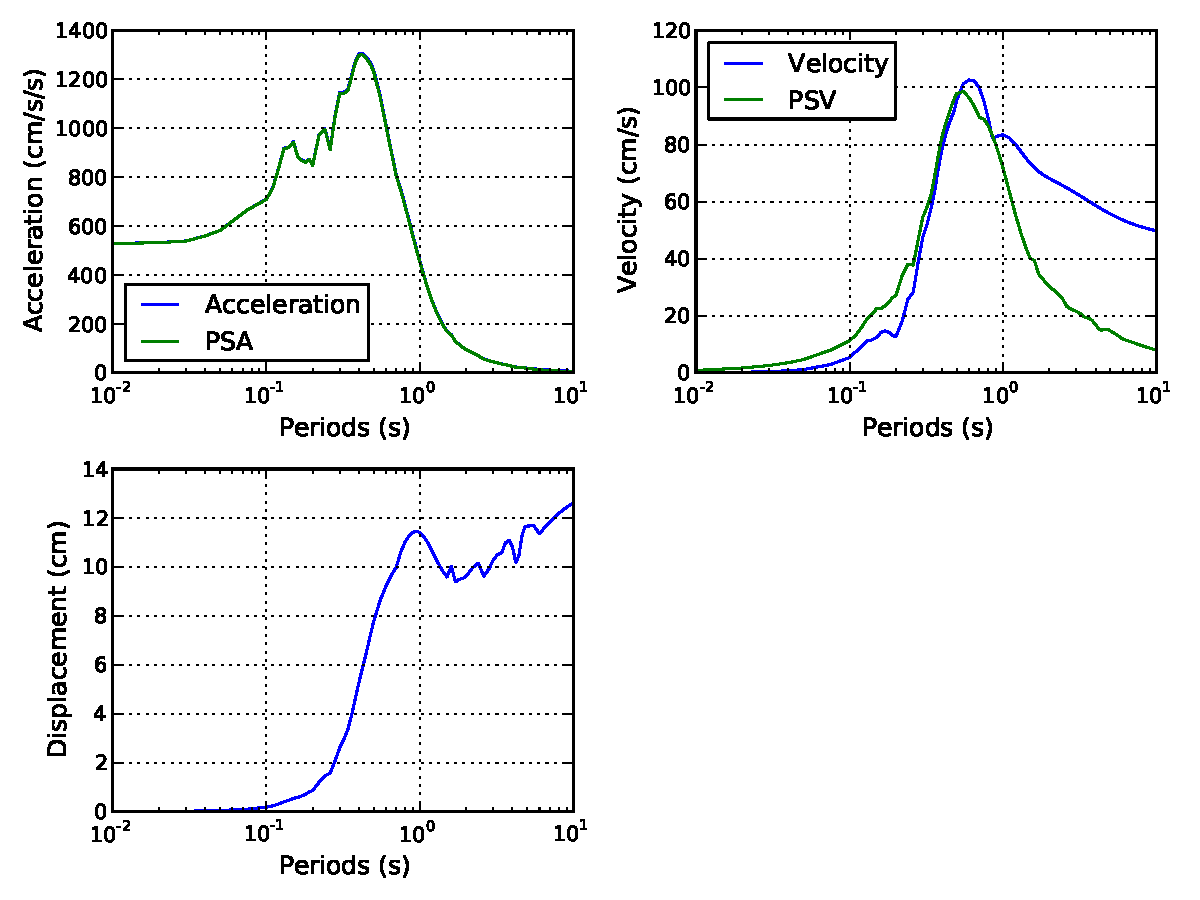
\includegraphics[width=\textwidth]{./figures/ims/response_newmark_beta.pdf}
	\caption{Full response spectra of the waveform shown in Figure \ref{fig:time_series}, calculated using the Newmark-$\beta$ method}
	\label{fig:newmark_beta}
\end{figure}
\begin{figure}[htb]
	\centering
		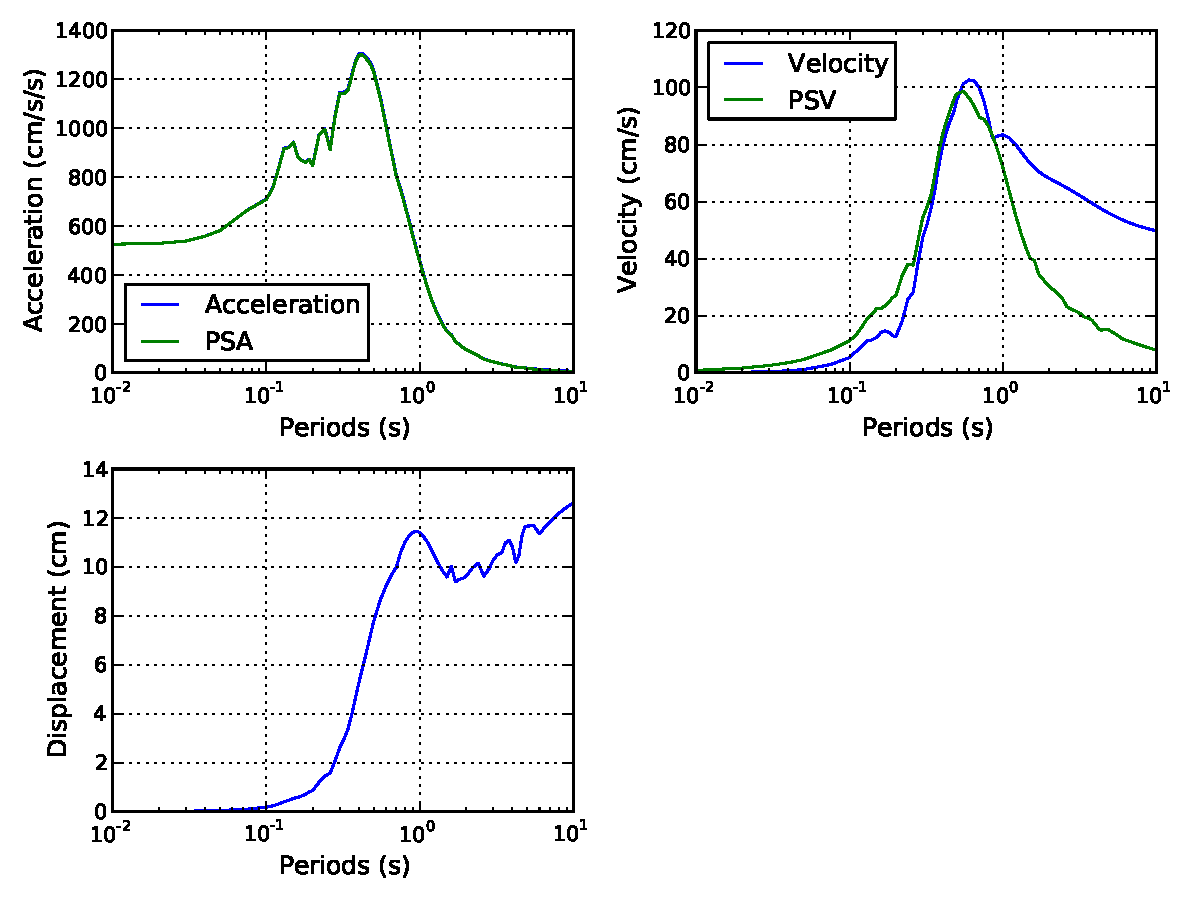
\includegraphics[width=\textwidth]{./figures/ims/response_nigam_jennings.pdf}
	\caption{Full response spectra of the waveform shown in Figure \ref{fig:time_series}, calculated using the Nigam \& Jennings (1969) method}
	\label{fig:nigam_jennings}
\end{figure}

\noindent where \verb=spectra= is the response spectra dictionary, \verb=axis_type= defines the type of axes: ``loglog'' (double logarithmic - the default), ``semilogx'' (logarithmic period axis), ``semilogy'' (logarithmic spectral response axis), ``linear'' (both axes linear). The function also takes the same keywords as the \verb=plot_time_series= method, i.e. \verb=figure_size=, \verb=filename=, \verb=filetype=, \verb=dpi=.

It can be seen from Figures  \ref{fig:newmark_beta} and \ref{fig:nigam_jennings} that both methods give very similar results.

\section{Combining Horizontal Components of Motion}
\label{sec:horizontal}

For a pair of horizontal records it is necessary to define a spectrum representing the ``horizontal'' component of ground motion. The manner in which the two horizontal components of motion are resolved can be treated in many different ways (cite: Douglas, 2003, ????; Beyer and Bommer etc.). The intensity measure tools contain various methods for combining horizontal response spectra. 

The first step in the application of these methods may be to extract the respective response spectra for the two horizontal components. This can be done as follows:

\begin{python}[frame=single]
spectra_x, spectra_y = ims.get_response_spectrum_pair(
    accel_x,
    time_step, # Time-step of x-component
    accel_y,
    time_step, # Time-step of y-component,
    periods,
    damping=0.05,
    units="cm/s/s",
    method="Nigam-Jennings")
\end{python}

In the case of the records demonstrated the time-step is the same for both horizontal components. If it is not the same, however, the response spectra can still be calculated.

Given the pair of records, \verb=spectra_x= ($Sa_x \left( {T, \xi} \right)$)and \verb=spectra_y= ($Sa_y \left( {T, \xi} \right)$), we can now obtain the following ``resolved'' horizontal spectra:

\begin{itemize}
\item \textbf{Geometric Mean}
    \begin{equation}
    Sa_{gm} \left( {T, \xi} \right) = \sqrt{Sa_x \left( {T, \xi} \right) \times Sa_y \left( {T, \xi} \right)}
    \end{equation}
    Calculated using the following command:
    \begin{python}
sa_gm = ims.geometric_mean_spectrum(spectra_x, spectra_y)
    \end{python}
    
\item \textbf{Arithmetic Mean}
    \begin{equation}
    Sa_{am} \left( {T, \xi} \right) = \frac{1}{2} \left( {Sa_x \left( {T, \xi} \right) + Sa_y \left( {T, \xi} \right)} \right)
    \end{equation}  
        Calculated using the following command:
    \begin{python}
sa_am = ims.arithmetic_mean_spectrum(spectra_x, spectra_y)
    \end{python}  

\item \textbf{Larger PGA}
    This simply returns the spectrum of the time series that gives the largest spectral acceleration. Calculated using the following command:
    \begin{python}
sa_larger = ims.larger_pga(spectra_x, spectra_y)
    \end{python}   

\item \textbf{Envelope}
    This returns a spectrum representing the larger of the two components for each period such that:
    \begin{equation}
    Sa_{env} \left( {T_i, \xi} \right) = \max\left( {Sa_x \left( {T_i, \xi} \right), Sa_y \left( {T_i, \xi} \right)} \right) \quad \text{for} \quad i = 1, 2, \ldots, N_{PERIODS}  
    \end{equation}
    \begin{python}
sa_env = ims.envelope(spectra_x, spectra_y)
    \end{python}  
\end{itemize}

In each of these cases the output of the function is a dictionary containing the same keys as that of the \verb=spectra=, but with the resolved horizontal values of each of the quantities. 

For the two spectra considered here, the geometric mean spectra and the envelope spectra are shown in Figures \ref{fig:geometric} and \ref{fig:envelope} respectively. 

\begin{figure}[htb]
	\centering
		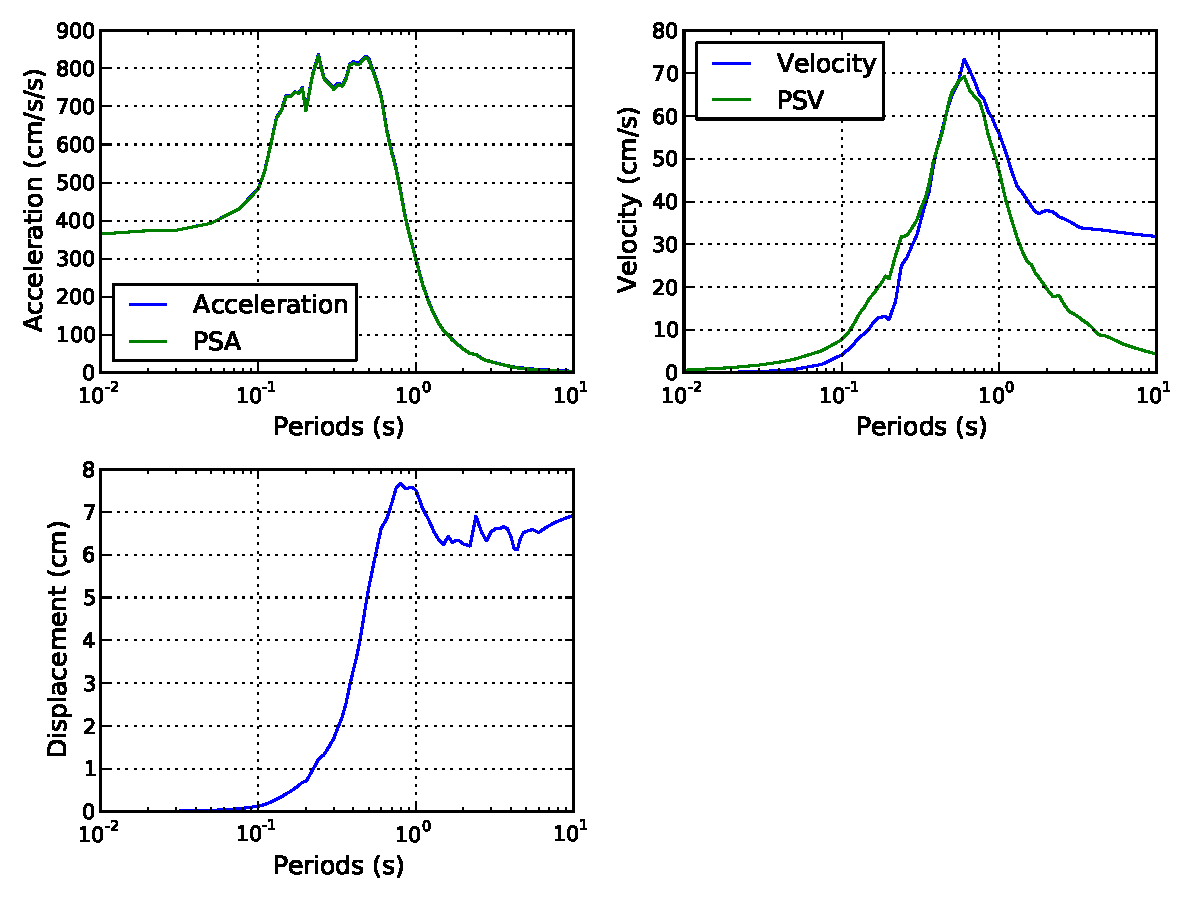
\includegraphics[width=12cm]{./figures/ims/geometric_mean_spectrum.pdf}
	\caption{Geometric mean spectra of the two horizontal records}
	\label{fig:geometric}
\end{figure}
\begin{figure}[htb]
	\centering
		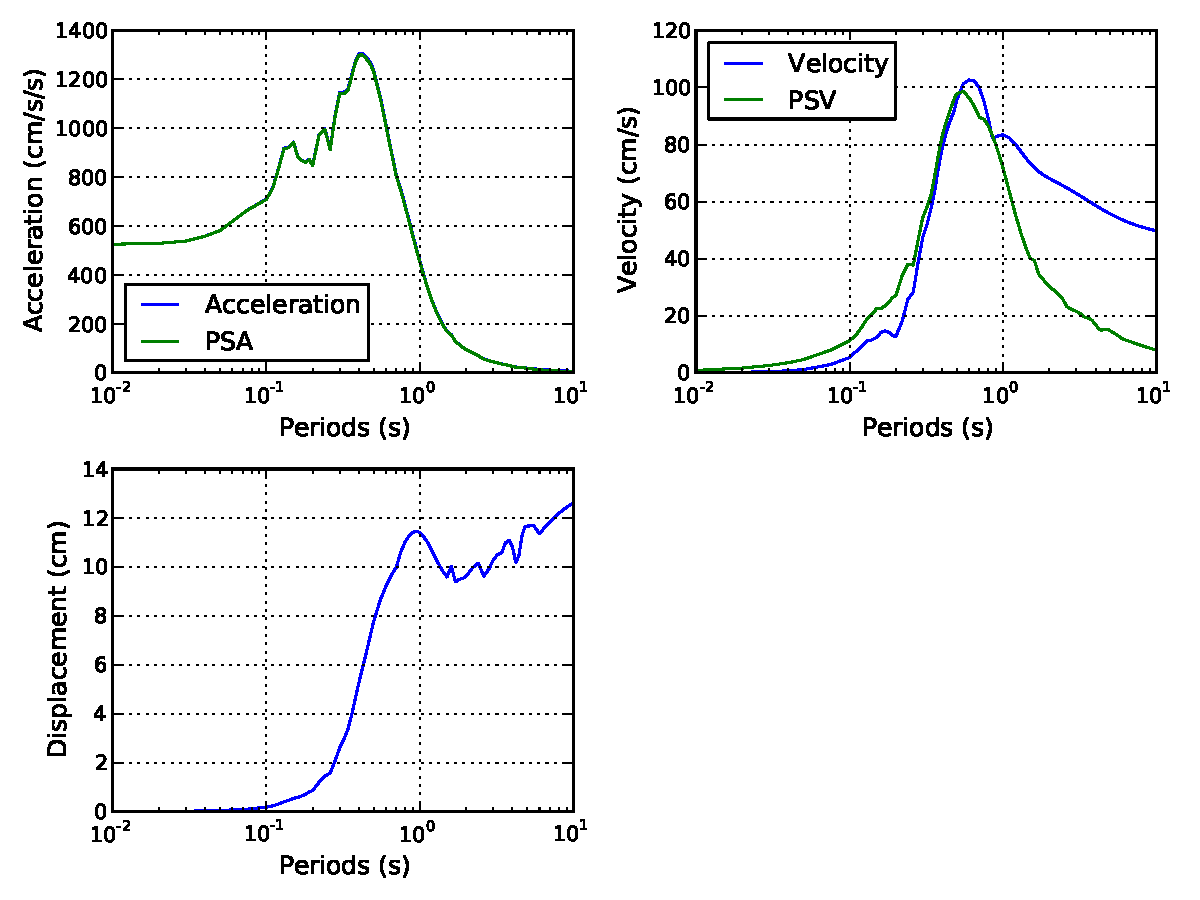
\includegraphics[width=12cm]{./figures/ims/envelope_spectrum.pdf}
	\caption{Envelope spectra of the two horizontal records}
	\label{fig:envelope}
\end{figure}

\section{Rotation of the Horizontal Records}

In some applications it may be necessary to rotate a pair of horizontal time series, either to orient them into fault-normal and fault-parallel components, or to some direction that may represent the most adverse for a particular structure. For two time series of equal duration and time series, the records can be rotated through angle $\theta$:

\begin{equation}
\begin{pmatrix}a_{x \left( {\theta} \right)} \left( t \right) \\ a_{y \left( {\theta} \right)} \left( t \right)\end{pmatrix} = \begin{bmatrix}\cos \theta & \sin \theta \\ -\sin \theta & \cos \theta \end{bmatrix} \begin{pmatrix}a_x\left( t \right) \\ a_y\left( t \right)\end{pmatrix}
\end{equation}

\noindent This can be achieved using the \verb=ims= tools:

\begin{python}[frame=single]
rot_hist_x, rot_hist_y = ims.rotate_horizontal(accel_x,
                                               accel_y,
                                               theta)
\end{python}

The incorporation of rotational tools permits the toolkit to calculate the ``orientation-dependent'' and ``orientation-independent'' geometric mean of a horizontal pair of records, as described in detail in CITE Boore et al (2006). The two quantities, \verb=GMRotDpp= and \verb=GMRotIpp= respectively, cannot be calculated from the two horizontal response spectra directly as other horizontal measures are. As they require rotation of time-series through non redundant angles, it is necessary to determine the response spectra for each rotation angle.

To calculate \verb=GMRotDpp= and \verb=GMRotIpp= run:

\begin{python}
gmrotd50 = ims.gmrotdpp(accel_x, time_step,
                        accel_y, time_step,
                        periods,
                        50.0, # Percentile
                        damping=0.05,
                        units="cm/s/s",
                        method="Nigam-Jennings")
gmroti50 = ims.gmrotipp(accel_x, time_step,
                        accel_y, time_step,
                        periods,
                        50.0, # Percentile
                        damping=0.05,
                        units="cm/s/s",
                        method="Nigam-Jennings")
\end{python}


\section{Adding Horizontal Components to the Database}

In the process of constructing the database of strong motion records it may often be prudent to compile the database in steps, of which the final one may often be the addition of the resolved horizontal components of the strong motion record. Depending on the data, and the required intensity measures, the calculation of horizontal spectra may be a (relatively) slow process with respect to the rest of the database construction. It is recommended that the database be constructed in the manner described in section \ref{sec:hdf5}, and then the resolved horizontal components added subsequently. To facilitate this a function is added to the database builder, which will add the desired horizontal ground motions to an existing database. An example is seen below:

\begin{python}[frame=single]
# Import the function add_horizontal_im
from smtk.sm_database_buider import add_horizontal_im
# Load in the database metadata file
import cPickle
database = cPickle.load(open("path/to/metadata.pkl", "r"))
# Choose the desired horizontal intensity measures
# The following will add the horizontal PGA, PGV
# Geometric mean spectrum, envelope spectrum and GMRotI50
im_list = ["PGA", "PGV", "Geometric", "Envelope", "GMRotI50"]
add_horizontal_im(database,
                  im_list, 
                  component="Geometric",
                  damping="05",
                  periods=[])
\end{python}

Depending on the size of the database this may take \textbf{many hours} to run (especially if rotational parameters are required). In this function the keyword \verb=component= refers only to the horizontal component of the scalar values. For the spectra, the type of horizontal component should be given in the intensity measure list. Note also that unlike the \verb=ims= and \verb=rsp= tools in which the damping is input as a floating point value, here it is input as a string. If not input by the user, the periods will be taken from the values stored in the x-component of the record. 



%----------------------------------------------------------------------------------------
%	CHAPTER 4
%----------------------------------------------------------------------------------------
\chapterimage{./figures/chapter_head_1.pdf} % Chapter heading image
\chapter{Comparing GMPEs: Trellis Plotting}
\label{chap:trellis}
\section{Trellis Plots: Advantages \& Limitations}
\label{sec:trellis}


\section{Trellis Plotting: The (Not So) Simple Way}
\label{sec:basic_trellis}


\section{Trellis Plotting: The Simple Way}
\label{sec:rupture_trellis}





%----------------------------------------------------------------------------------------
%	CHAPTER 5
%----------------------------------------------------------------------------------------
\chapterimage{./figures/chapter_head_1.pdf} % Chapter heading image
\chapter{Comparing Models and Observations}
\label{chap:residuals}
\section{GMPE Residuals}
\label{sec:residuals}

\subsection{Definition of the GMPE Residuals}

Arguably one of the most critical processes in GMPE selection, and GMPE weighting in an epistemic uncertainty analysis, is the comparison of the GMPEs against set of ground motions for the region of application. These analyses can serve several purposes. The first is to understand the extent to which the GMPE of interest can represents the local properties of source, path and site scaling of the ground motion. In modelling both the expected ground motion and the aleatory varibility, each GMPE is a probability distribution in which a ground motion $y_{ij}$ at recorded location $j$, originating from event $i$, is characteristed by a lognormal distribution:

\begin{equation}
\log y_{ij} = \mu \left( {m_i, r_{ij}, \mathbf{\theta_{ij}}} \right) + z_{T, ij}\sigma_T
\label{eq:gmpe_total}
\end{equation}

\noindent where $\mu \left( {m_i, r_{ij}, \mathbf{\theta_{ij}}} \right)$ is the expected ground motion from an event of magnitude $m_i$, recorded at a distance $r_{ij}$, where $\mathbf{\theta_{ij}}$ corresponds to various other model parameters relevant to the model in question (e.g., site amplification, basin response, hanging wall scaling etc.). The total uncertainty ($z_{T, ij}$) is therefore modelled as a normal distribution with a mean of zero and a standard deviation of $\sigma_T$. The term $z_{T, ij}$ is therefore the ``total'' normalised residual of the $j^{th}$ recording from the $i^{th}$ event:

\begin{equation}
z_{T, ij} = \frac{\log \left( {y_{ij}} \right) - \mu \left( {m_i, r_{ij}, \mathbf{\theta_{ij}}} \right)}{\sigma_T}
\label{eq:total_residual}
\end{equation}

For most GMPEs, however, the a random effects regression process is used to derive the coefficients of the model. This divides the total residual term into an inter-event component $\delta_{E, i}$ and an the intra-event component $\delta_{A, ij}$, such that equation \label{eq:gmpe} can be written as:

\begin{equation}
\log y_{ij} = \mu \left( {m_i, r_{ij}, \mathbf{\theta_{ij}}} \right) +  \delta_{E, i} + \delta_{A, ij}
\label{eq:gmpe_randeff}
\end{equation}

The inter-event residual is normally distributed with a mean of zero and a standard deviation of $\tau$, and likewise the intra-event residual is normally distributed with a zero mean and a standard deviation of $\sigma$. 
Consequently equation \ref{eq:gmpe_randeff} can be finally written as:

\begin{equation}
\log y_{ij} = \mu \left( {m_i, r_{ij}, \mathbf{\theta_{ij}}} \right) +  z_{E,i}\tau + z_{A, ij}\sigma
\label{eq:gmpe_re_resid}
\end{equation}

Where $z_{E, i}$ and $z_{A_ ij}$ are the normalised inter- and intra-event residuals respectively. Following the random effects definition of cite{AbrhamsonYoungs1992}, the inter-event term is defined via:

\begin{equation}
\delta_{E, i} = z_{E, i} \tau = \frac{\tau^2 \sum\limits_{j = 1}^{n_i} \left( {y_{ij} - \mu \left( {m_i, r_{ij}, \mathbf{\theta_{ij}}} \right)}\right)}{n_i \tau^2 + \sigma^2}
\label{eq:inter_res}
\end{equation}

\noindent where $n_i$ is the number of records observed from event $i$. The intra-event residual the follows:

\begin{equation}
\delta_{A, ij} = z_{A, ij}\sigma = \log y_{ij} - \mu \left( {m_i, r_{ij}, \mathbf{\theta_{ij}}} \right) - z_{E, i}\tau
\label{eq:intra_res}
\end{equation}

\subsection{Residual analysis in the GMPE-SMTK}

The GMPE-SMTK offers the ability to compare observed ground motions with the GMPE model predictions using the GMPE implementations found inside OpenQuake. This is a particularly powerful tool as it permits, possibly for the first time, a hazard modeller to undertake the GMPE comparison using the exact same GMPE implementation found inside the seismic hazard software. This ensures consistency between, for example, the definitions of the distance metrics, as well as allowing the GMPE-SMTK to inherit the comprehensive test coverage that is fundamental to the OpenQuake software. 

Several key sets of tools can be found within the GMPE-SMTK to allow the modeller not only to explore particular features of the GMPE residuals, but also to undertake quantitative analysis of the overall fit of each GMPE to observed strong motion data. All the analyses undertaken will, by default, analyse the total residual, the inter-event residual and the intra-event residual, following the approach described in cite(StaffordEtAl2008). If the GMPE in question does not provide coefficients to define the inter- and intra-event residual only the total residual term will be considered.

The GMPE-SMTK provides two sets of tools. The first tool set contains the tools to undertake the analysis of residuals, and/or the model fit. These tools are found in the module \\ \verb=smtk.residuals.gmpe_residuals=. The second set will provide the visualisation and plotting functionalities. These are found in the \verb=smtk.residuals.residual_plotter= module. In the following examples we will refer to these modules as \verb=res= and \verb=rspl= respectively, and they can be imported via:

\begin{python}[frame=single]
import smtk.residuals.gmpe_residuals as res
import smtk.residuals.residual_plotter as rspl
\end{python}

To generate a set of ground motion residuals the tools require three pieces of information: a ground motion database (as an instance of the \verb=smtk.sm_database.GroundMotionDatabase= class), a list of the required GMPEs and a list of the required intensity measures. In the following examples we consider a set of strong motion records recorded in Italy and compare four GMPEs (BooreAtkinson2008, AkkarBommer2010, AkkarCagnan2010, AkkarEtAl2014) and four intensity measures (PGA, $Sa \left( {0.2 s} \right)$, $Sa \left( {1.0 s} \right)$, $Sa \left( {2.0 s} \right)$). Typically, these will be set-up as follows:

\begin{python}[frame=single]
# Import CPickle
import cPickle
# Import the database
sm_database = cPickle.loads(open("path/to/metadata.pkl", "r"))
# Define the list of GMPEs
gmpe_list = ["BooreAtkinson2008",
             "AkkarBommer2010",
             "AkkarCagnan2010",
             "AkkarEtAlRjb2014"]
# Define the list of intensity measures
imt_list = ["PGA", "SA(0.2)", "SA(1.0)", "SA(2.0)"] 
\end{python}

For undertaking simple analysis of residuals simply run:

\begin{python}[frame=single]
# Set-up the residual calculator
resid1 = res.Residuals(gmpe_list, imts)
# Run the residual calculator
resid1.get_residuals(sm_database)
\end{python}

When run, the class \verb=Residuals= will hold an attribute \verb=residuals=, which will contain a set of nested python dictionaries in which the corresponding residual values are stored. To retrieve the residual values for a specific GMPE and intensity measure then type:

\begin{python}
res_data = resid1.residuals["GMPE Name"]["IM Name"]["Type"]
\end{python}

where, ``GMPE Name'' is the name of the GMPE specified in the input list, ``IM Name'' is the name of the intensity measure (as specified in the input list) and ``Type'' is one of ``Total'', ``Inter event'' or ``Intra event'' (note the syntax - the keys are case sensitive). The residuals will then be a single vector of residual values for that specific GMPE, IM and residual type.
  

\section{Basic Trends in Residuals}
\label{sec:residual_trends}

One of the simplest means of comparing observations with the models is via the use of histograms of the residual terms $z_T$, $z_{E, i}$ and $z_A{ij}$ from the observed records with respect to the GMPE. These help identify the general tendency of the GMPE with respect to the records. From the definitions described in \ref{sec:residuals} it follows that for a GMPE to represent a good fit to a set of records each of the normalised residual distributions should match closely to a standard normal distribution (i.e with a mean of zero and standard deviation of 1.0). Differences in the mean of the residuals may indicate a tendency for the GMPE to predict higher or lower values than those observed in records, whilst differences in the standard deviation may suggest an over- or underestimation of the variability of the ground motions.

Basic histograms of the residuals of a GMPE can be created using the \verb=rspl= tool \verb=ResidualPlot=. For the GMPEs listed in previously the following command will produce the four sets of histogram plots for the trend in PGA residuals shown in Figure \ref{fig:pga_resids} and, for $Sa \left( {1.0 s} \right)$ using Akkar et al (2014) only in Figure \ref{fig:sa1_res_akkar2014}.

\begin{python}
# Boore & Atkinson (2008)
rspl.ResidualPlot(resid1, "BooreAtkinson2008", "PGA",
                  filename="path/to/image.png",
                  filetype="png")
# Akkar & Bommer (2010)
rspl.ResidualPlot(resid1, "AkkarBommer2010", "PGA")
# Akkar & Cagnan (2010)
rspl.ResidualPlot(resid1, "AkkarCagnan2010", "PGA")
# Akker et al. (2014)
rspl.ResidualPlot(resid1, "AkkarEtAlRjb2014", "PGA")
# Akker et al. (2014) - Sa (1.0 s)
rspl.ResidualPlot(resid1, "AkkarEtAlRjb2014", "Sa(1.0)")
\end{python}

\begin{figure}[htb]
  \centering
  \begin{subfigure}[b]{0.49\textwidth}
      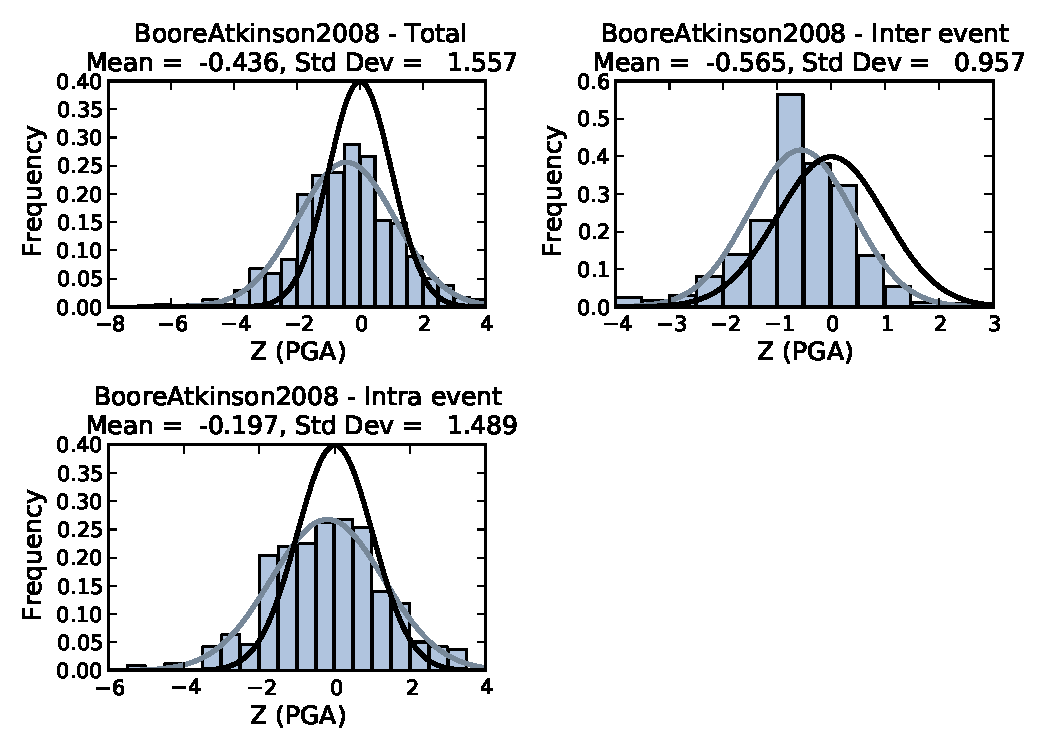
\includegraphics[width=\textwidth]{./figures/residuals/BA2008_Residuals_PGA.pdf}
      \caption{citeBooreAtkinson2008 model}
      \label{fig:pga_res_ba2008}
  \end{subfigure}
    \begin{subfigure}[b]{0.49\textwidth}
      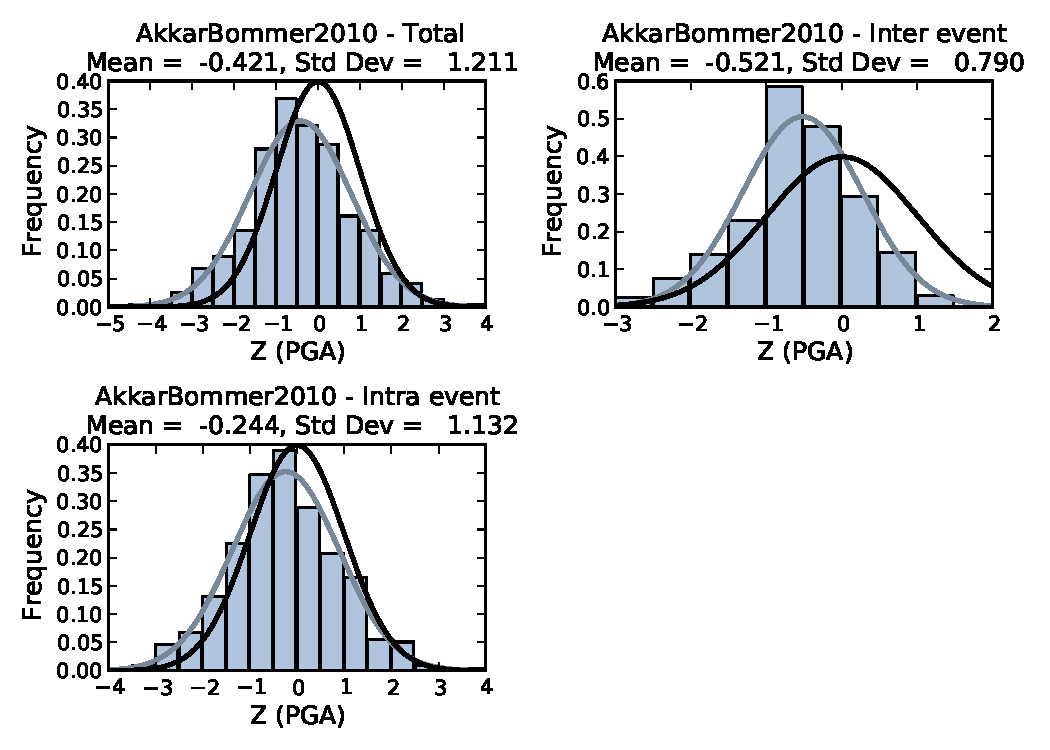
\includegraphics[width=\textwidth]{./figures/residuals/AB2010_Residuals_PGA.pdf}
      \caption{citeAkkarBommer2010 model}
      \label{fig:pga_res_ab2010}
  \end{subfigure}
    \begin{subfigure}[b]{0.49\textwidth}
      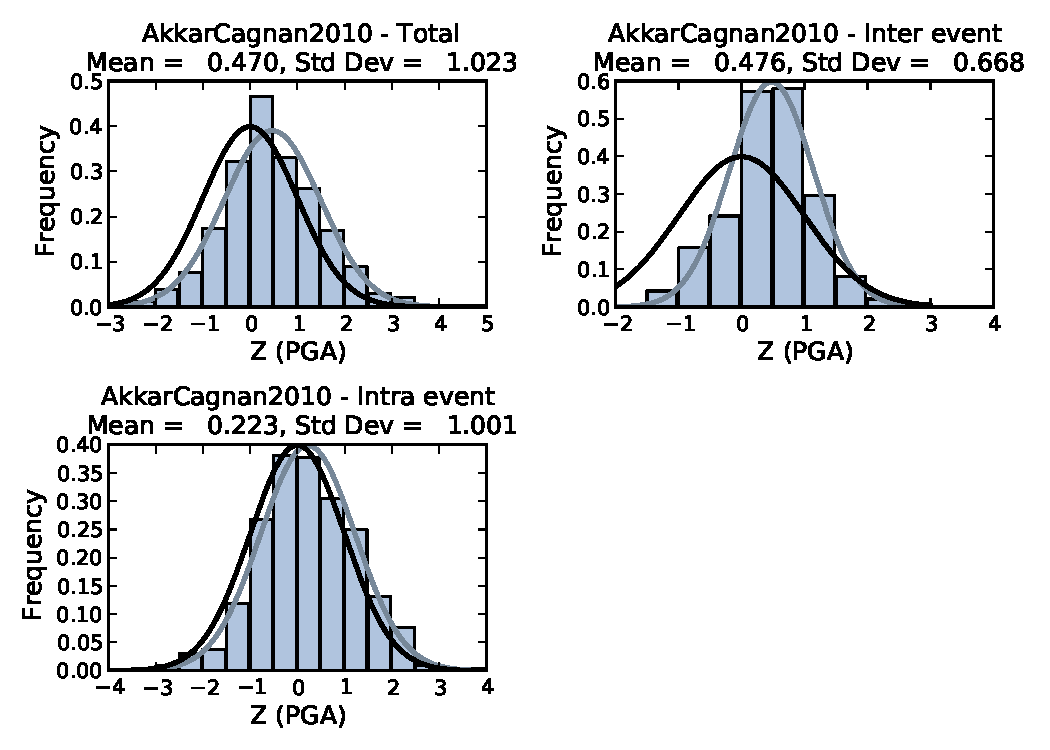
\includegraphics[width=\textwidth]{./figures/residuals/AC2010_Residuals_PGA.pdf}
      \caption{citeAkkarCagnan2010 model}
      \label{fig:pga_res_ac2010}
  \end{subfigure}
      \begin{subfigure}[b]{0.49\textwidth}
      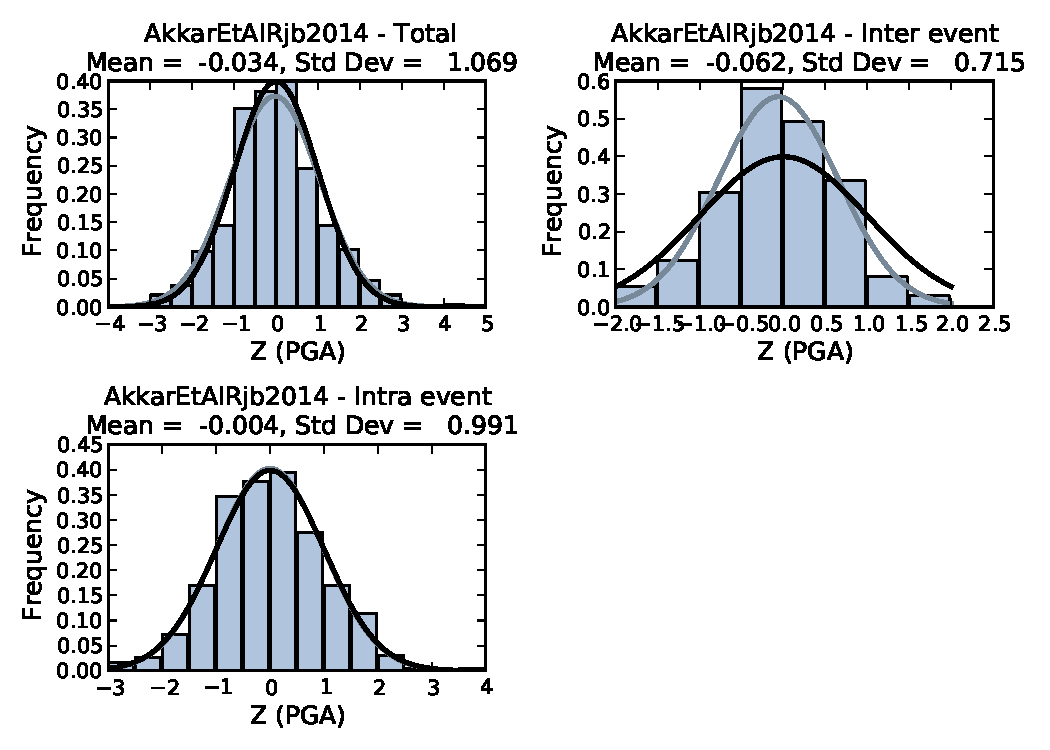
\includegraphics[width=\textwidth]{./figures/residuals/Akkar2014_Residuals_PGA.pdf}
     \caption{citeAkkarEtAl2014 model}
      \label{fig:pga_res_akkar2014}
  \end{subfigure}
  \caption{PGA residual distribution for the record set. The grey line indicates the probability density function fit to the data, whilst the black line indicates the standard normal density function}
  \label{fig:pga_resids}
\end{figure}

\begin{figure}[htb]
	\centering
		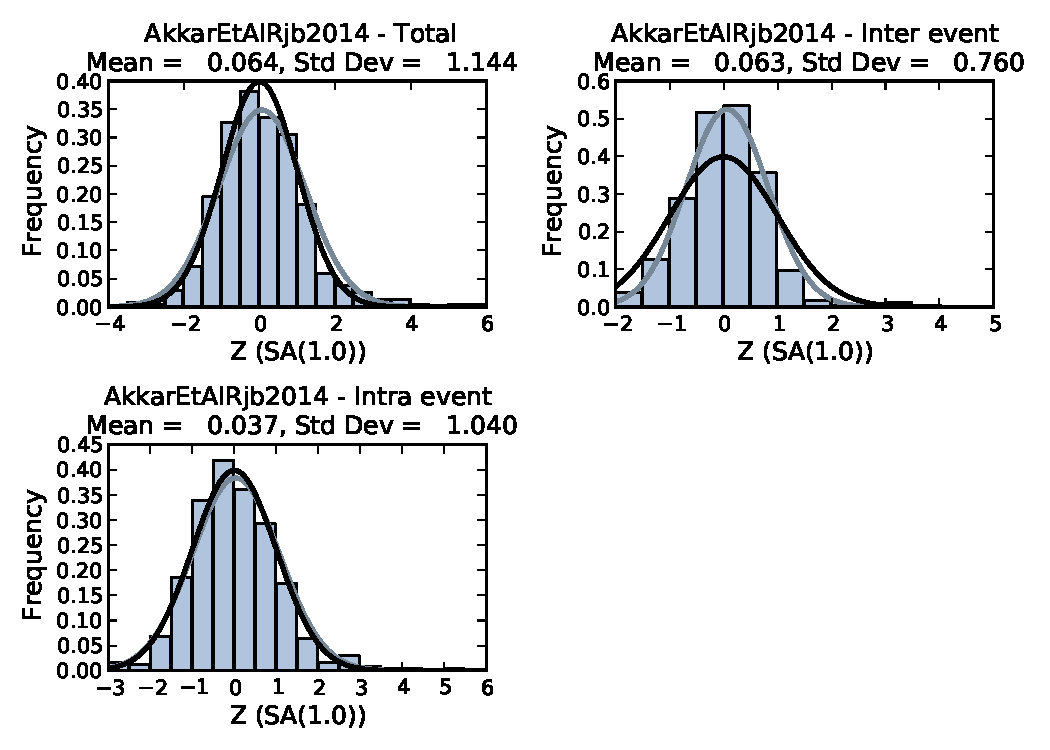
\includegraphics[width=0.6\textwidth]{./figures/residuals/Akkar2014_Residuals_Sa1.pdf}
	\caption{PGA residual distribution for the record set using the Akkar et al. (2014) GMPE}
	\label{fig:sa1_res_akkar2014}
\end{figure}

Figures \ref{fig:pga_resids} and \ref{fig:sa1_res_akkar2014} shows a relatively discernible set of trends. Consider just the \cite{boore2008} model for PGA (Figure \ref{fig:pga_res_ba2008}). Each of the residuals have a mean less than zero, significantly so in the case of the inter-event residual. This indicates that in general the \cite{boore2008} model is predicts higher ground motions than those observed in the records and most of this can be attributed to the inter-event term. The distributions also show a greater spread than expected from the model, as demonstrated by the standard deviation greater than unity. In this case it is the intra-event residuals that show a greater spread than expected, whilst spread in the inter-event residuals is in better agreement with the model. In contrast the Akkar et al. (2014)  GMPE (from which the current records form part of the generating data set) show a much closer agreement with the records (as expected). It is seen that that the distribution of the normalised total residuals is very close to the standard normal distribution; a trend that is matched in the intra-event residuals. Similarly in the inter-event residuals the mean value is close to zero, and only the spread of the model shows a difference, in this case showing a smaller variance than expected from the model. This is to be expected as the current dataset is based on exclusively Italian records (predominantly extensional events, with only a few thrust or oblique slip records), whereas the GMPE was fit to a full set of European and Middle Eastern records, thus incorporating a greater variability of mechanism types than just the Italian subset. The same trend can be seen in the residuals for $Sa \left( {1.0 s} \right)$. 

\section{The Likelihood Model (TOCITE Scherbaum et al., 2004)}
\label{sec:lh_model}

The basic residual trends can help understand where biases may be present in the model with respect to the record set, but they do not necessarily provide a quantitative indication of the total fit of the model to the record. One possibility to do this (others will presented later in the chapter) is to consider the overall goodness-of-fit of the model to the predictions. SCHERBAUM ETAL 2004 consider the probability that the absolute value of a random sample from the normalised distribution to fall into the interval between the modulus of a particular observation $|z_0|$ and infinity.

\begin{equation}
u \left( {z_0} \right) = \frac{1}{2} Erf\left( {\frac{z_0}{\sqrt{2}}, \infty} \right)
\end{equation}

The total ``likelihood'' of a particular value is given by:

\begin{equation}
LH \left( {|z_0|} \right) = 2 \cdot u \left( {|z_0|} \right) = Erf \left( {\frac{|z_0|}{\sqrt{2}}, \infty} \right)
\end{equation}

As indicated in SCHERBAUM ETAL 2004 the the $LH$ value should reach a value of $1$ for $|z_0|=0$ (i.e. the mean of the distribution), and should tend to zero for observations further away from the mean. Therefore, if the model assumptions are matched exactly by a set of observations then the $LH \left( {|z_0|} \right)$ values should be distributed evenly between 0 and 1, with a median value of 0.5. 

The GMPE-SMTK can produce histograms of the $LH$ value for the ground motion observations using the \verb=res.Likelihood= and \verb=rspl.LikelihoodPlot= tools. The \verb=res.Likeihood= tool operates in the same manner as the \verb=res.Residuals= tool; therefore to run the likelihood analysis one follows the same approach:

\begin{python}[frame=single]
# Set-up the likelihood calculator
lh1 = res.Likelihood(gmpe_list, imts)
# Run the residual calculator
lh1.get_residuals(sm_database)
\end{python}

Histograms of the $LH$ values (and their median estimates) for the four GMPEs for PGA are shown in Figure \ref{fig:pga_lh}, and for only Akkar et al. (2014) for $Sa \left( {1.0 s} \right)$ in Figure \ref{fig:sa1_lh_akkar2014} . These can be generated with the following command:

\begin{python}
# Boore & Atkinson (2008)
rspl.LikelihoodPlot(lh1, "BooreAtkinson2008", "PGA",
                    filename="path/to/image.png",
                    filetype="png")
# Akkar & Bommer (2010)
rspl.LikelihoodPlot(lh1, "AkkarBommer2010", "PGA")
# Akkar & Cagnan (2010)
rspl.LikelihoodPlot(lh1, "AkkarCagnan2010", "PGA")
# Akker et al. (2014)
rspl.LikelihoodPlot(lh1, "AkkarEtAlRjb2014", "PGA")
# Akker et al. (2014) - Sa (1.0 s)
rspl.LikelihoodPlot(lh1, "AkkarEtAlRjb2014", "Sa(1.0)")
\end{python}

\begin{figure}[htb]
  \centering
  \begin{subfigure}[b]{0.49\textwidth}
      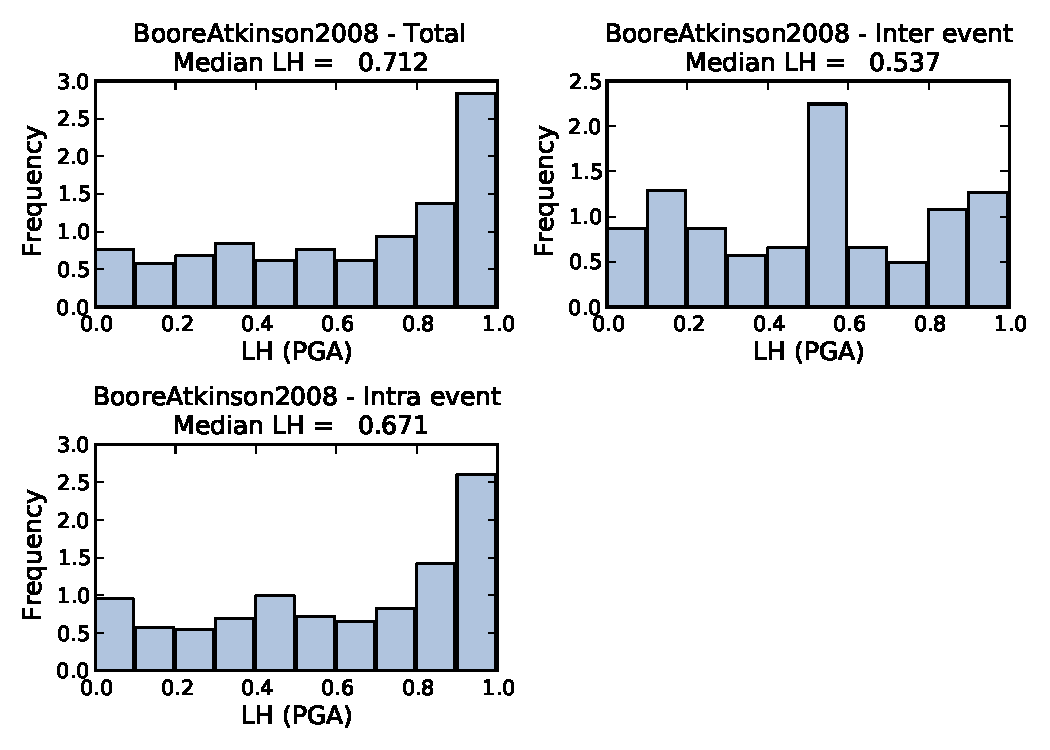
\includegraphics[width=\textwidth]{./figures/residuals/BA2008_LH_PGA.pdf}
      \caption{citeBooreAtkinson2008 model}
      \label{fig:pga_lh_ba2008}
  \end{subfigure}
    \begin{subfigure}[b]{0.49\textwidth}
      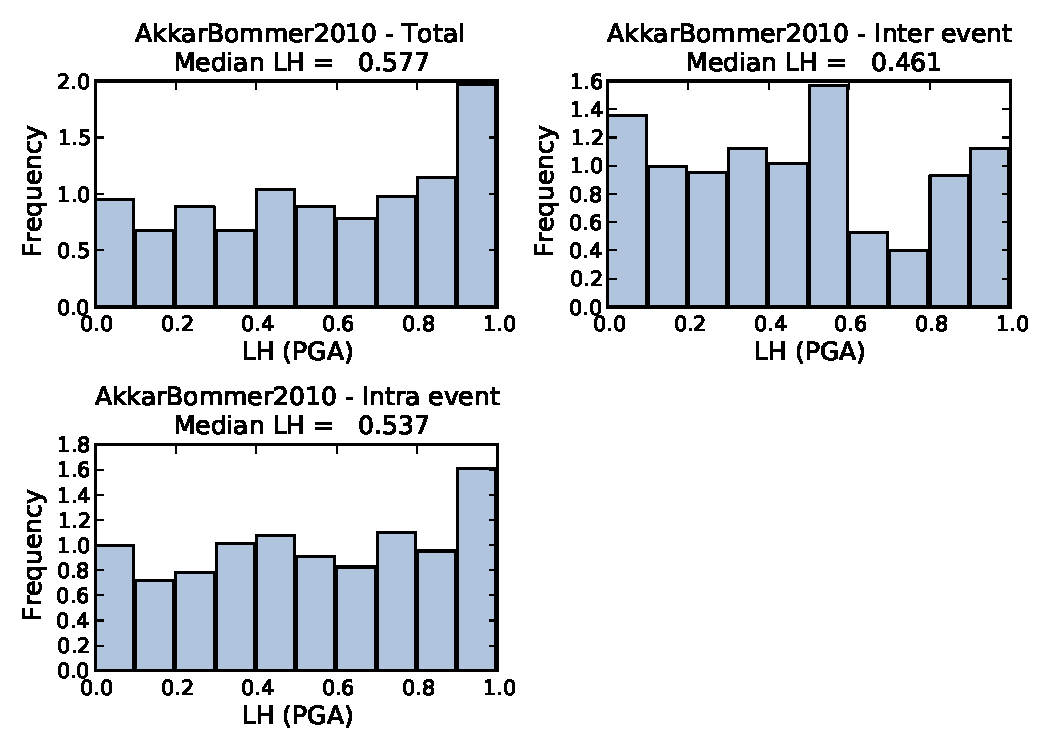
\includegraphics[width=\textwidth]{./figures/residuals/AB2010_LH_PGA.pdf}
      \caption{citeAkkarBommer2010 model}
      \label{fig:pga_lh_ab2010}
  \end{subfigure}
    \begin{subfigure}[b]{0.49\textwidth}
      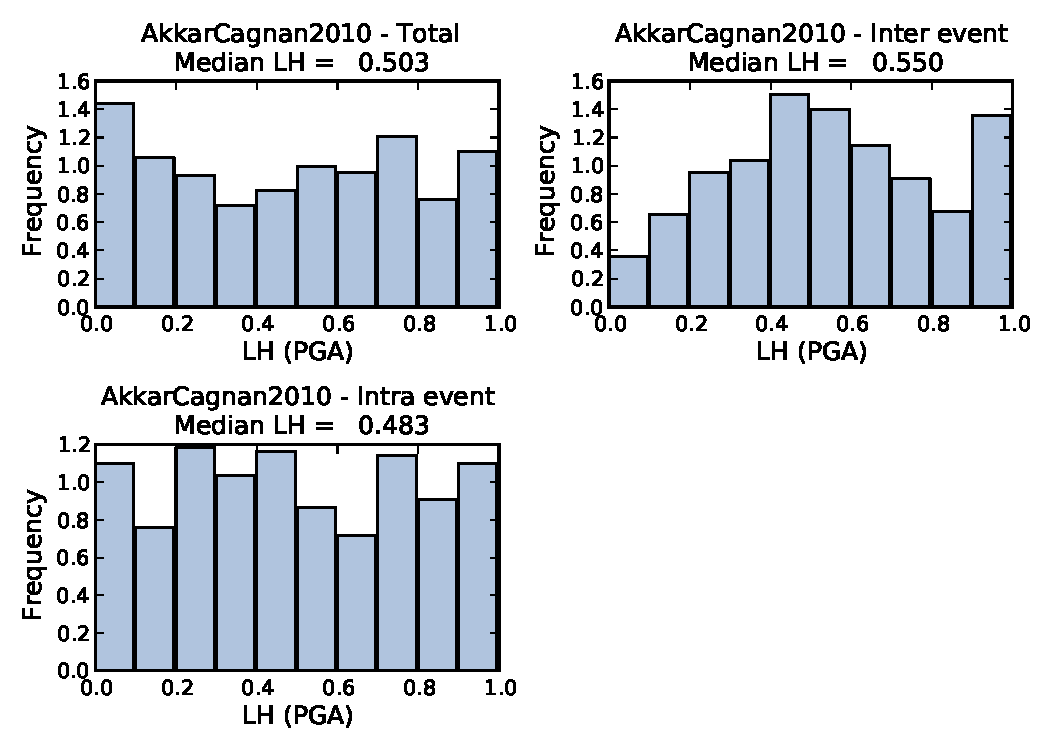
\includegraphics[width=\textwidth]{./figures/residuals/AC2010_LH_PGA.pdf}
      \caption{citeAkkarCagnan2010 model}
      \label{fig:pga_lh_ac2010}
  \end{subfigure}
      \begin{subfigure}[b]{0.49\textwidth}
      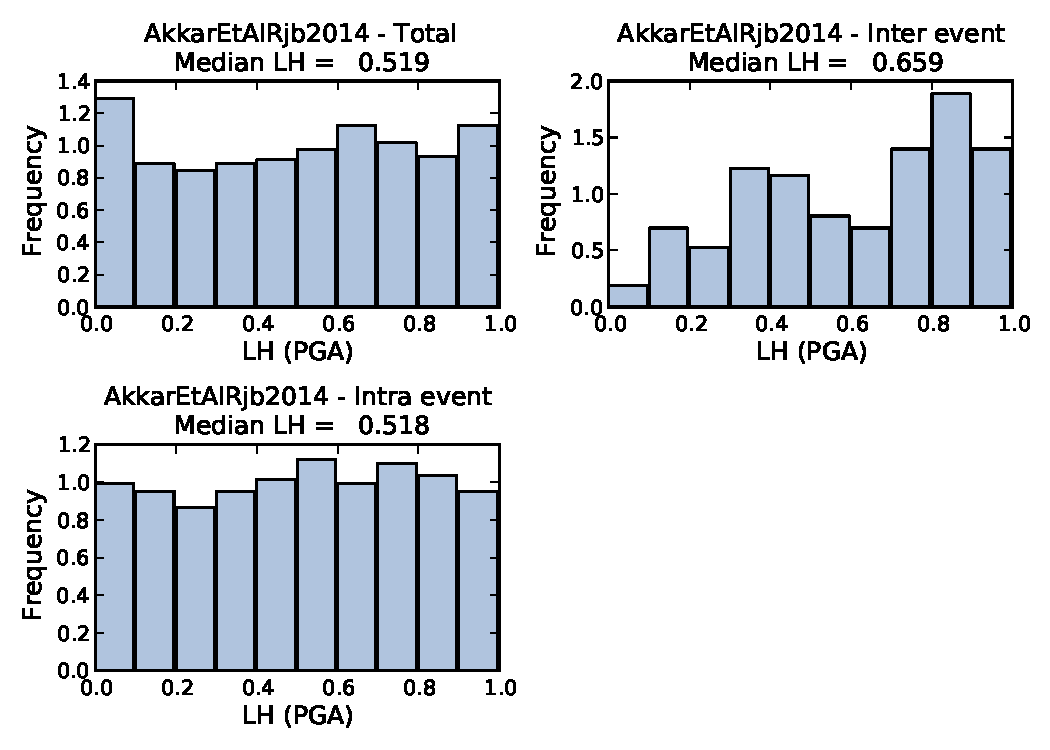
\includegraphics[width=\textwidth]{./figures/residuals/Akkar2014_LH_PGA.pdf}
     \caption{citeAkkarEtAl2014 model}
      \label{fig:pga_lh_akkar2014}
  \end{subfigure}
  \caption{$LH$ distribution for the observed PGA set}
  \label{fig:pga_lh}
\end{figure}

\begin{figure}[htb]
	\centering
		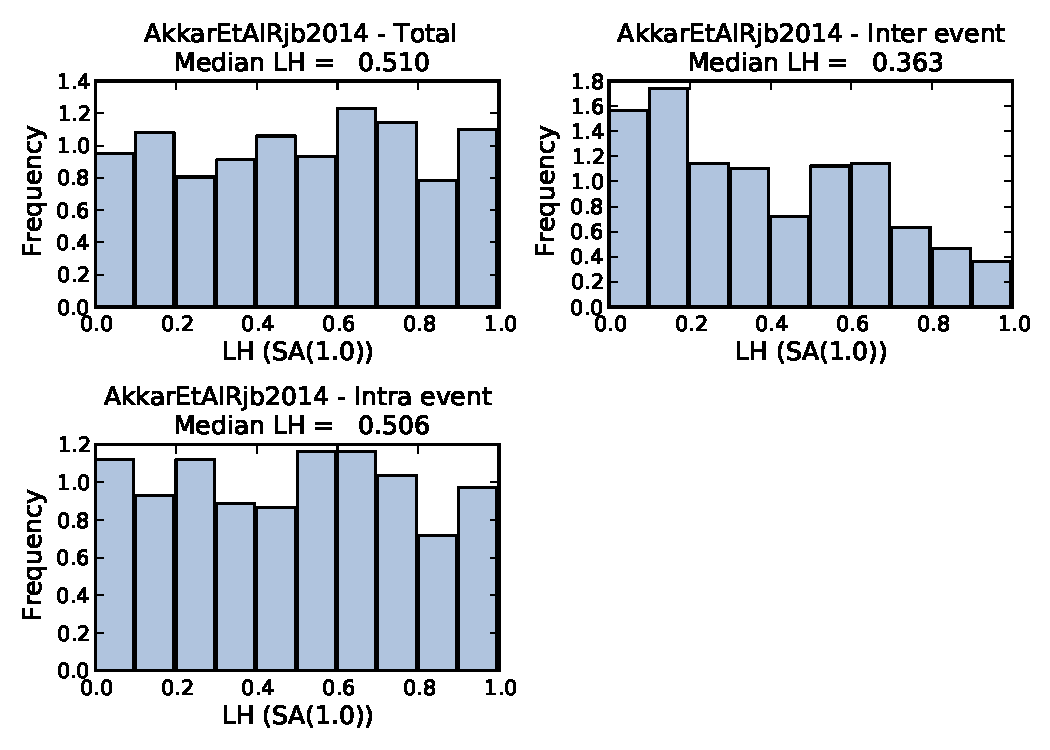
\includegraphics[width=0.6\textwidth]{./figures/residuals/Akkar2014_LH_Sa1.pdf}
	\caption{$LH$ distribution for the observed $Sa \left( {1.0 s} \right)$ set using the Akkar et al. (2014) GMPE}
	\label{fig:sa1_lh_akkar2014}
\end{figure}

In general the trends seen in Figure \ref{fig:pga_resids} are visible in the $LH$ histograms in the manner described in SCHERBAUM ETAL 2004. In the \cite{boore2008} model intra-event and total residuals showed a greater variance than predicted by the GMPE, a trend that tends to result in $LH$ values closer to zero than 1. For the Akkar et al. (2014) GMPE both the total and inter-event residuals are generally evenly distributed between 0 and 1, with a median of close to 0.5, indicating a good agreement between the model and observations. The inter-event residuals show a smaller range than that expected by the model and so the $LH$ values are closer to 1.0 (the distances from the mean are smaller than expected). 

\section{Residual Trends with Predictor Variables}
\label{sec:predictor_trends}

The analysis of the residuals shown in sections \ref{sec:residual_trends} and \ref{sec:lh_model} provide useful insights into the overall fit of a GMPE to a set of observations. They do not necessarily provide a clear indication as to which elements of the model contribute to the misfit. Or, to frame it differently, they do not necessarily indicate where the GMPEs may be biased with respect to the predictor variables of the observations. To analysis this it is necessary to understand if, and where, the GMPE residuals show clear trends with respect to the predictor variables. These trends can indicate those elements of the source/site scaling and attenuation process for which the GMPE is biased.

The GMPE-SMTK offers several methods to visualise the trends of the GMPE residuals with the following predictor variables:
\begin{enumerate}
\item Magnitude
\item Distance
\item $V_{S30}$
\item Hypocentral Depth
\end{enumerate}

\subsubsection{Trends with Magnitude}

To view the trends with magnitude for a set of ground motion residuals the \verb=rspl= toolset contains the function \verb=ResidualWithMagnitude=. Figure \ref{fig:mag_resid} shows the residual trends in magnitude for the \cite{boore2008} and Akkar et al. (2014) GMPEs for PGA and $Sa \left( {1.0 s} \right)$. These figures were generated with the following commands:

\begin{python}[frame=single]
# Boore & Atkinson (2008)  - PGA
rspl.ResidualWithMagnitude(resid1,  # Residuals
                           "BooreAtkinson2008",  # GMPE
                           "PGA",   # Intensity Measure
                           filename="path/to/image.png",
                           filetype="png")
# Akkar et al. (2014)  - PGA
rspl.ResidualWithMagnitude(resid1, "AkkarEtAlRjb2014", "PGA") 
# Boore & Atkinson (2008)  - Sa (1.0)
rspl.ResidualWithMagnitude(resid1, "BooreAtkinson2008",
                          "Sa(1.0)") 
# Akkar et al. (2014)  - Sa (1.0)
rspl.ResidualWithMagnitude(resid1, "AkkarEtAlRjb2014",
                          "Sa(1.0)")                         
\end{python}

As shown in Figure \ref{fig:mag_resid}, and in subsequent figures, a linear model is fit to the observed residual trends. The significance of the trend is measured via the ``p-value'', reported in the figure header. This indicates the probability observing the measured trend in the residuals assuming a null hypothesis of no trend (i.e. zero gradient). Consequently a smaller ``p-value'' indicates a more significant trend, assuming (loosely) that statistically significant trends might be those with a ``p-value'' smaller than 0.1. If the magnitude scaling is largely unbiased with respect to the GMPE it is expected that no significant linear trend can be observed the plot of residuals with magnitude. This is the case for the Akkar et al. (2014) GMPE in which no statistically significant trend is observed with respect to magnitude. For the Boore and Atkinson (2008) model a statistically significant trend is visible in the inter-event residuals. For PGA this trend is negative, suggesting that the GMPE is predicting higher than observed ground motions for the larget magnitudes, whilst for $Sa \left( {1.0 s} \right)$ the opposite is true, indicating the GMPE is predicting lower than expected ground motions at higher magnitudes.

\begin{figure}[htb]
  \centering
  \begin{subfigure}[b]{0.49\textwidth}
      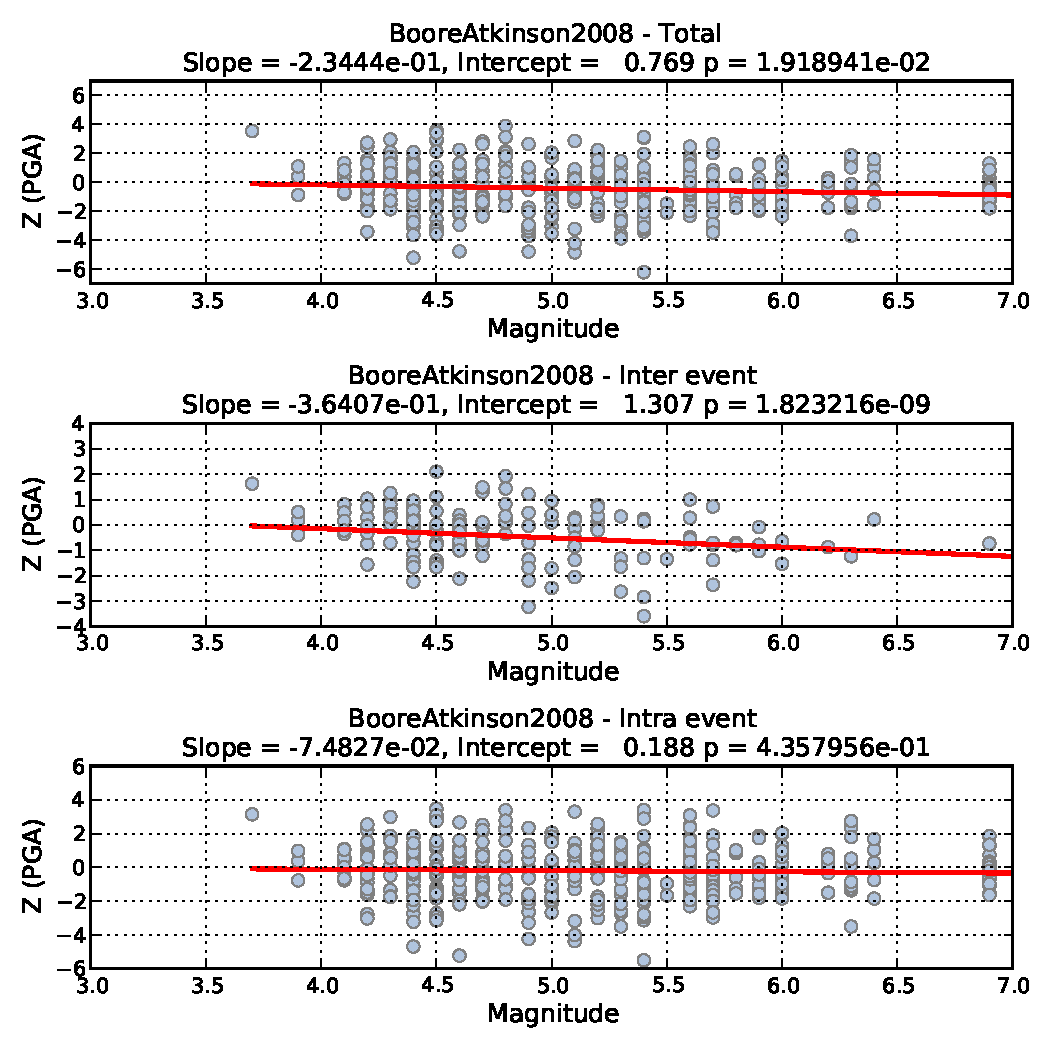
\includegraphics[width=\textwidth]{./figures/residuals/BA2008_Magnitude_PGA.pdf}
      \caption{citeBooreAtkinson2008 model - PGA}
      \label{fig:pga_mag_ba2008}
  \end{subfigure}
    \begin{subfigure}[b]{0.49\textwidth}
      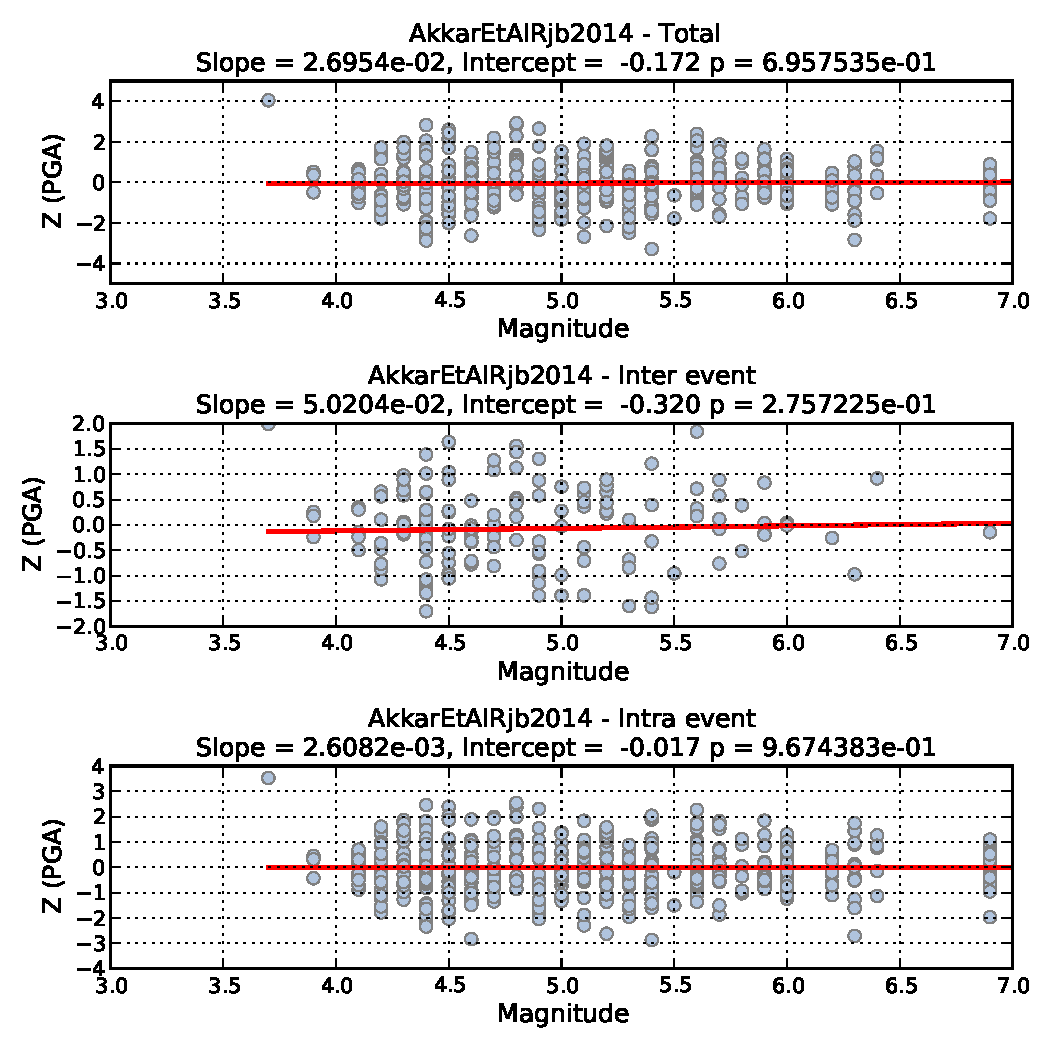
\includegraphics[width=\textwidth]{./figures/residuals/Akkar2014_Magnitude_PGA.pdf}
      \caption{citeAkkarEtAl2014 model - PGA}
      \label{fig:pga_mag_akkar2014}
  \end{subfigure}
    \begin{subfigure}[b]{0.49\textwidth}
      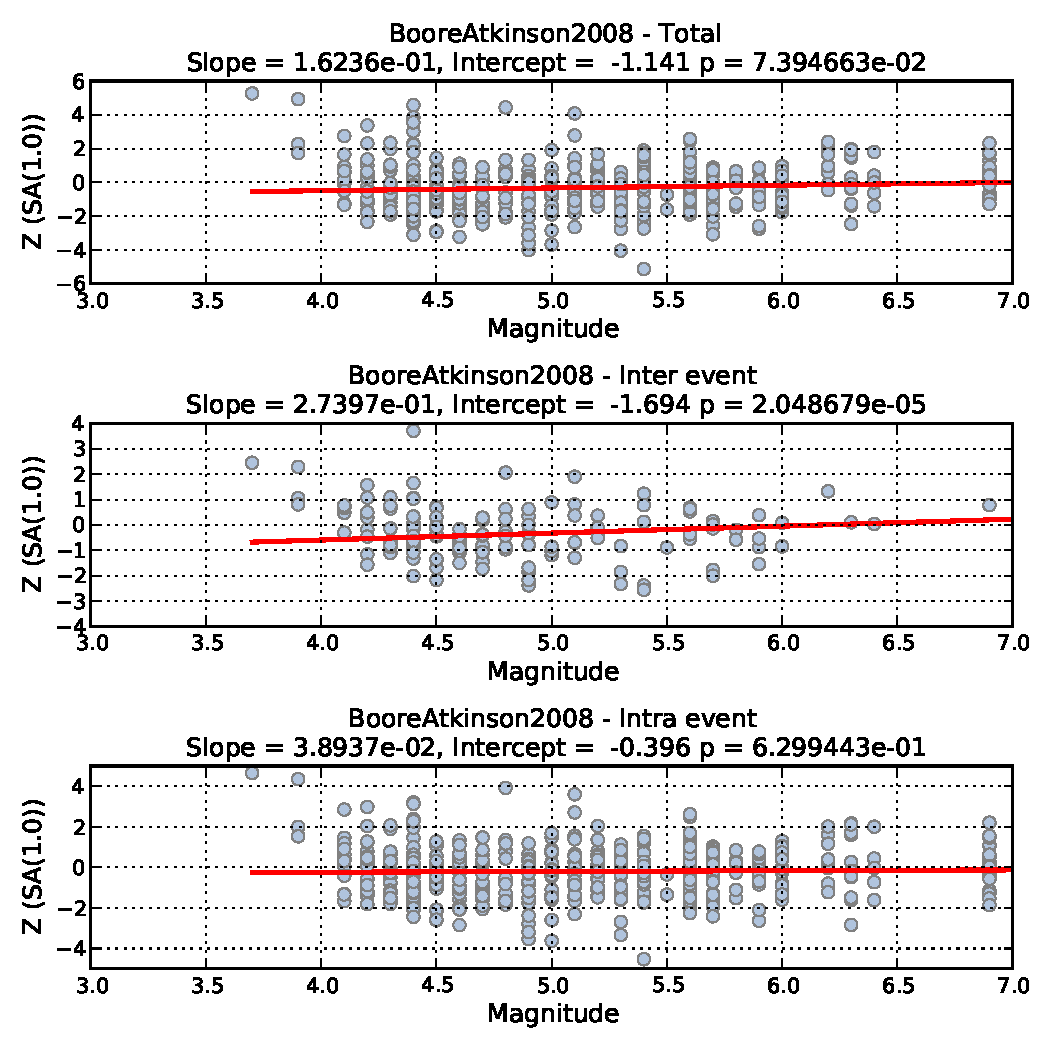
\includegraphics[width=\textwidth]{./figures/residuals/BA2008_Magnitude_Sa1.pdf}
      \caption{citeBooreAtkinson2008 model - $Sa \left( {1.0 s} \right)$}
      \label{fig:sa1_mag_ba2008}
  \end{subfigure}
      \begin{subfigure}[b]{0.49\textwidth}
      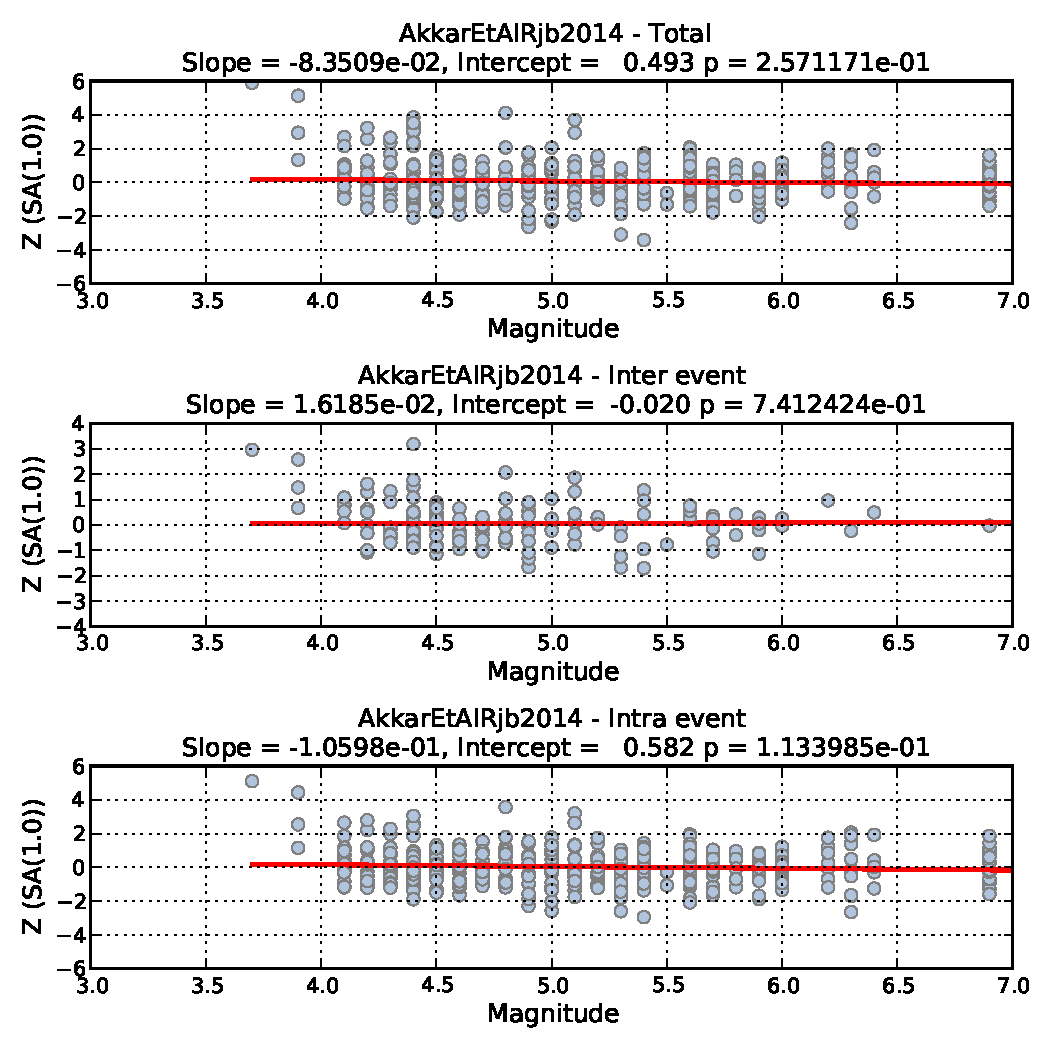
\includegraphics[width=\textwidth]{./figures/residuals/Akkar2014_Magnitude_Sa1.pdf}
     \caption{citeAkkarEtAl2014 model - $Sa \left( {1.0 s} \right)$}
      \label{fig:sa1_mag_akkar2014}
  \end{subfigure}
  \caption{Residual trends with magnitude for the observed PGA and $Sa \left( {1.0 s} \right)$ records}
  \label{fig:mag_resid}
\end{figure}


\subsubsection{Trends with Distance}

To observe how well the GMPE compares to the distance attenuation properties in a set of records the \verb=rspl= tools provide the method \verb=ResidualWithDistance=. Plots of residuals with distance for the same GMPEs and intensity measures considered in Figure \ref{fig:mag_resid} are shown in Figure \ref{fig:dist_resid}. These are generated using the following commands:

\begin{python}[frame=single]
# Boore & Atkinson (2008)  - PGA
rspl.ResidualWithDistance(resid1,  # Residuals
                           "BooreAtkinson2008",  # GMPE
                           "PGA",   # Intensity Measure
                           distance_type="rjb"
                           plot_type="linear",
                           filename="path/to/image.png",
                           filetype="png")
# Akkar et al. (2014)  - PGA
rspl.ResidualWithDistance(resid1, "AkkarEtAlRjb2014",
                          "PGA", distance_type="rjb",
                          plot_type="linear") 
# Boore & Atkinson (2008)  - Sa (1.0)
rspl.ResidualWithDistance(resid1, "BooreAtkinson2008",
                          "Sa(1.0)", distance_type="rjb",
                          plot_type="linear") 
# Akkar et al. (2014)  - Sa (1.0)
rspl.ResidualWithDistance(resid1, "AkkarEtAlRjb2014",
                          "Sa(1.0)", distance_type="rjb",
                          plot_type="linear")                         
\end{python}

The input arguments are identical to the \verb=ResidualwithMagnitude= tool, with the exception of the \verb=distance_type= and \verb=plot_type= keywords. The \verb=distance_type= determines the distance measure used for visualisation, whilst the \verb=plot_type= keyword indicates whether to plot the distance values on a logarithmic axis (``\verb=log='') or a linear axis (``\verb=linear=''). A logarithmic axis is preferred by default.

In contrast to the residual trends with magnitude, it is evident in Figure \ref{fig:dist_resid} that statistically significant trends with distance exist for both GMPEs. This can be clearly seen in the intra-event residual, which shows a negative trend in the residuals, a trend that is more pronounced for the Boore \& Atkinson (2008) model. This indicates that both models underestimate the degree of attenuation in the ground motions observed in Italy, as both models predict higher ground motion at greater distances than those observed in the strong motion records. 

\begin{figure}[htb]
  \centering
  \begin{subfigure}[b]{0.49\textwidth}
      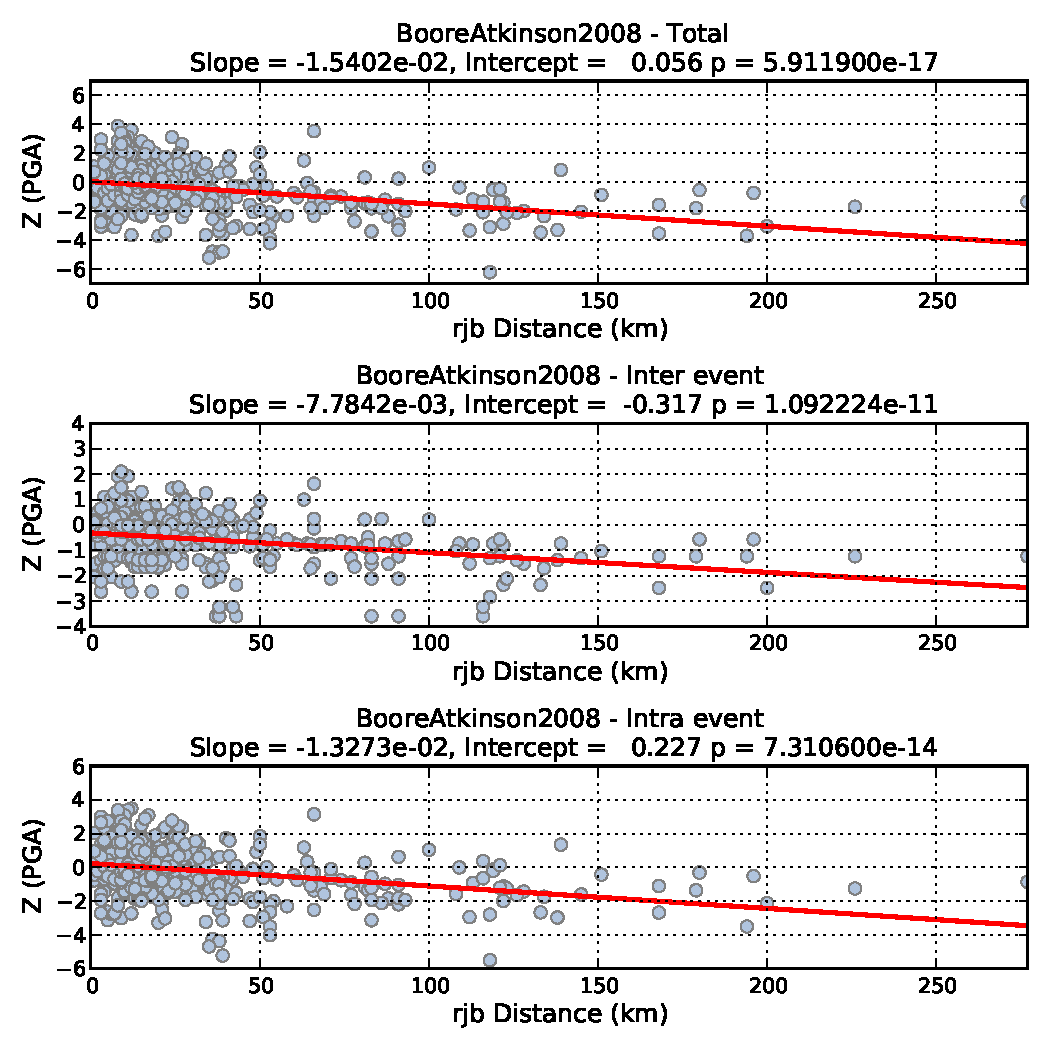
\includegraphics[width=\textwidth]{./figures/residuals/BA2008_Distance_PGA.pdf}
      \caption{citeBooreAtkinson2008 model - PGA}
      \label{fig:pga_dist_ba2008}
  \end{subfigure}
    \begin{subfigure}[b]{0.49\textwidth}
      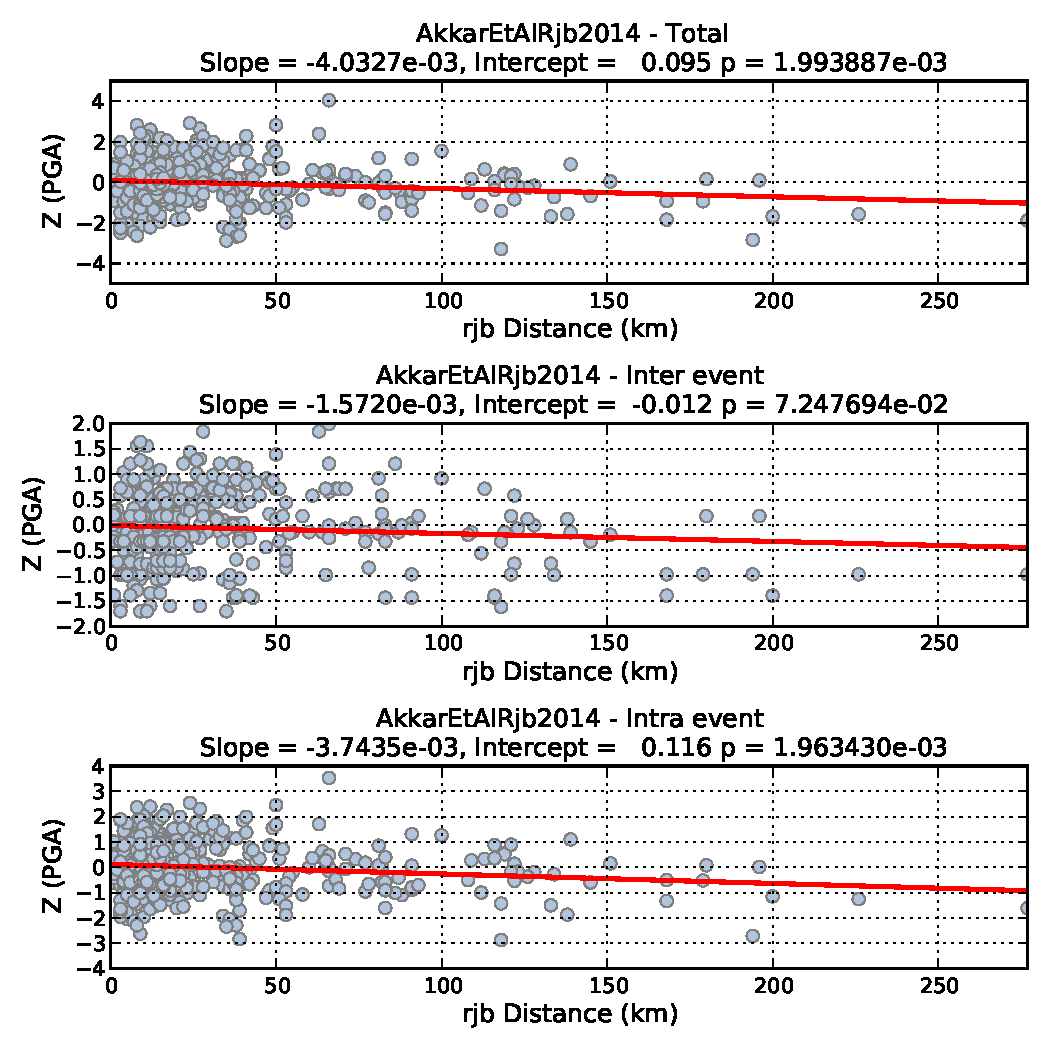
\includegraphics[width=\textwidth]{./figures/residuals/Akkar2014_Distance_PGA.pdf}
      \caption{citeAkkarEtAl2014 model - PGA}
      \label{fig:pga_dist_akkar2014}
  \end{subfigure}
    \begin{subfigure}[b]{0.49\textwidth}
      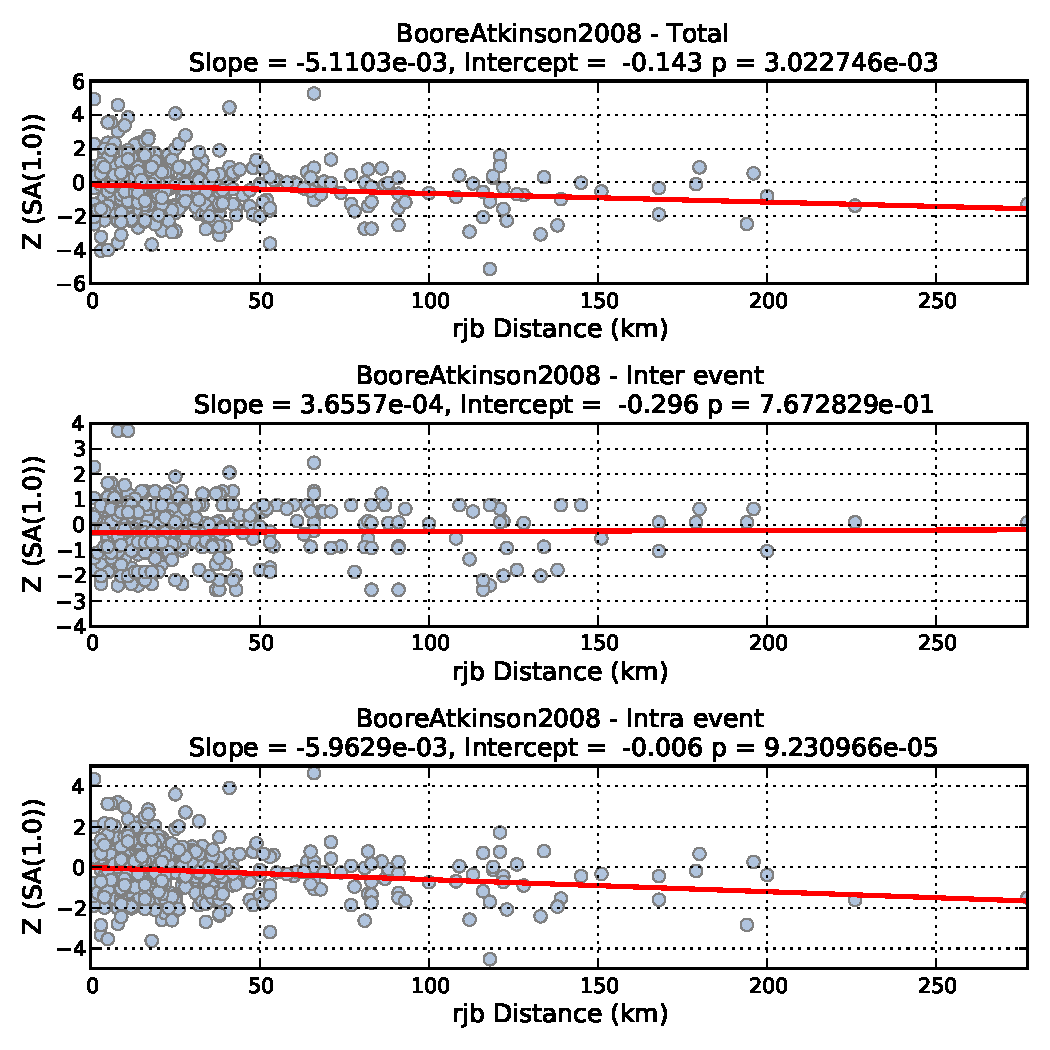
\includegraphics[width=\textwidth]{./figures/residuals/BA2008_Distance_Sa1.pdf}
      \caption{citeBooreAtkinson2008 model - $Sa \left( {1.0 s} \right)$}
      \label{fig:sa1_dist_ba2008}
  \end{subfigure}
      \begin{subfigure}[b]{0.49\textwidth}
      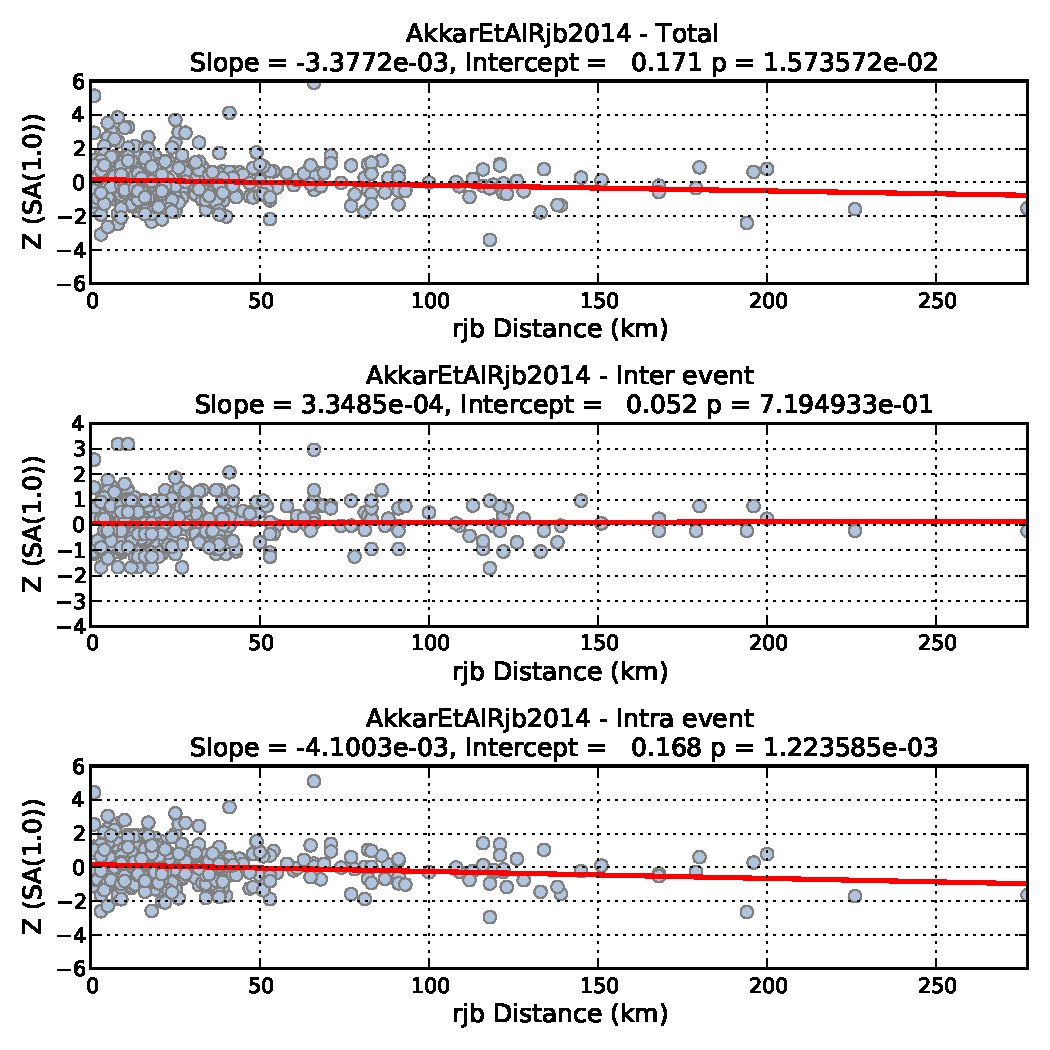
\includegraphics[width=\textwidth]{./figures/residuals/Akkar2014_Distance_Sa1.pdf}
     \caption{citeAkkarEtAl2014 model - $Sa \left( {1.0 s} \right)$}
      \label{fig:sa1_dist_akkar2014}
  \end{subfigure}
  \caption{Residual trends with Joyner-Boore distance for the observed PGA and $Sa \left( {1.0 s} \right)$ records}
  \label{fig:dist_resid}
\end{figure}

\subsubsection{Trends with $V_{S30}$}

The usage of the \verb=rspl= tool to visualise residual trends with $V_{S30}$ (\verb=ResidualWithVs30=) is generally the same as the tools for the magnitude and distance. So for the same GMPEs and intensity measures considered previously, the following commands are used to produce the plot of residuals against $V_{S30}$ for the same record set, shown in Figure \ref{fig:vs30_resid}:
 
 \begin{python}[frame=single]
# Boore & Atkinson (2008)  - PGA
rspl.ResidualWithVs30(resid1,  # Residuals
                      "BooreAtkinson2008",  # GMPE
                      "PGA",   # Intensity Measure
                      filename="path/to/image.png",
                      filetype="png")
# Akkar et al. (2014)  - PGA
rspl.ResidualWithVs30(resid1, "AkkarEtAlRjb2014", "PGA") 
# Boore & Atkinson (2008)  - Sa (1.0)
rspl.ResidualWithVs30(resid1, "BooreAtkinson2008", "Sa(1.0)") 
# Akkar et al. (2014)  - Sa (1.0)
rspl.ResidualWithVs30(resid1, "AkkarEtAlRjb2014", "Sa(1.0)")                         
\end{python}

Once again in both the GMPEs and for both intensity measures there are statistically significant trends in the residuals with $V_{S30}$. In most cases the trends are positive, with a negative intercept, indicating that the GMPEs are predicting higher than expected ground motions on softer soils (i.e. lower $V_{s30}$) for the selected stations.

\begin{figure}[htb]
  \centering
  \begin{subfigure}[b]{0.49\textwidth}
      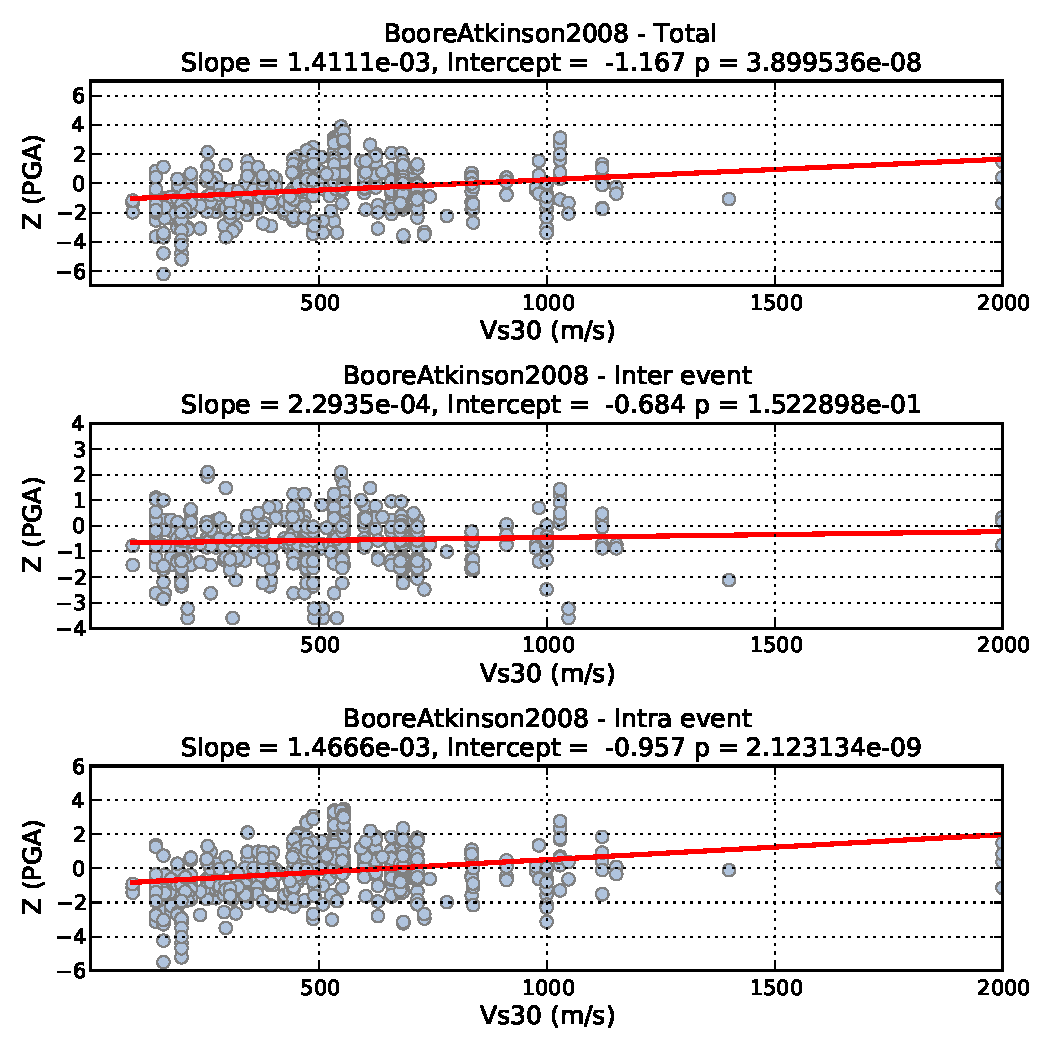
\includegraphics[width=\textwidth]{./figures/residuals/BA2008_Vs30_PGA.pdf}
      \caption{citeAkkarEtAl2014 model - PGA}
      \label{fig:pga_vs30_ba2008}
  \end{subfigure}
    \begin{subfigure}[b]{0.49\textwidth}
      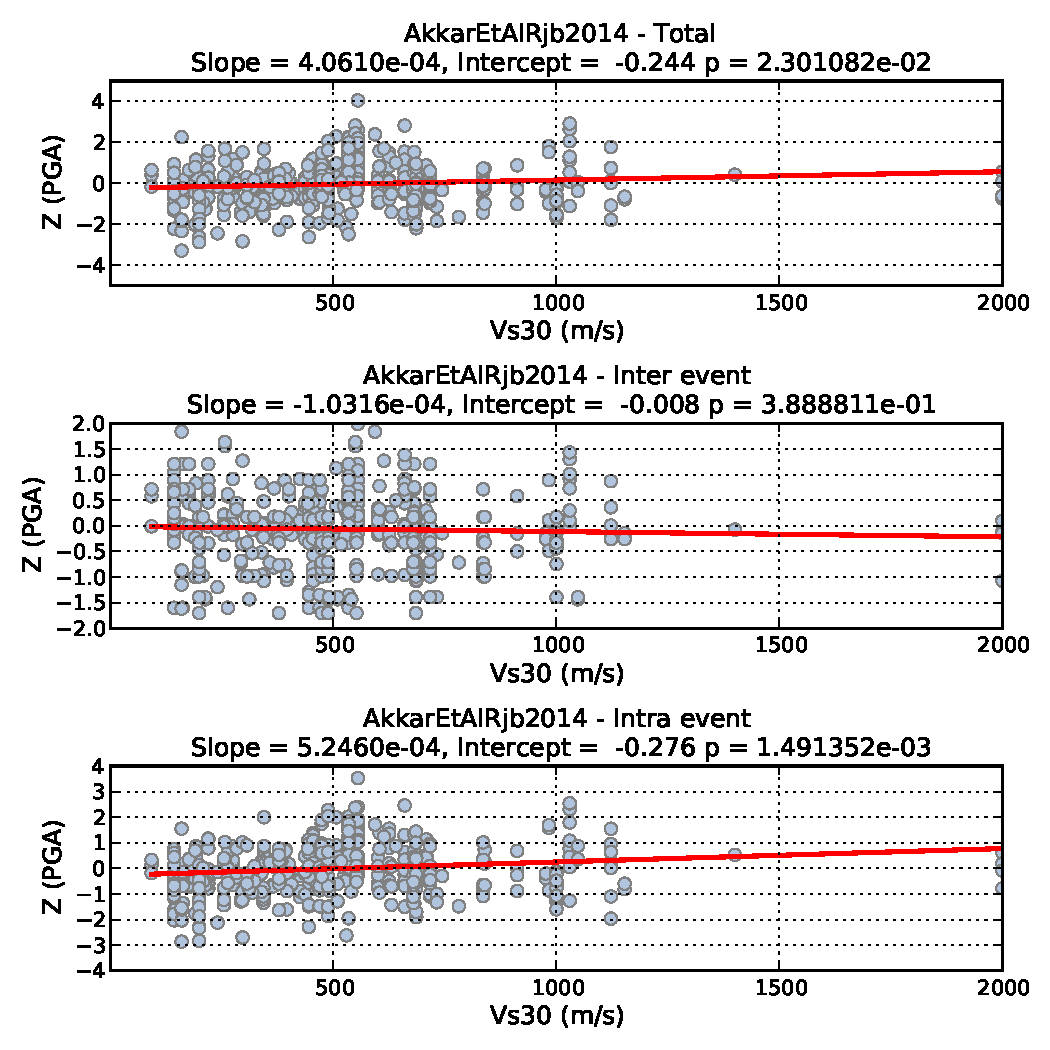
\includegraphics[width=\textwidth]{./figures/residuals/Akkar2014_Vs30_PGA.pdf}
      \caption{citeAkkarBommer2010 model - PGA}
      \label{fig:pga_vs30_akkar2014}
  \end{subfigure}
    \begin{subfigure}[b]{0.49\textwidth}
      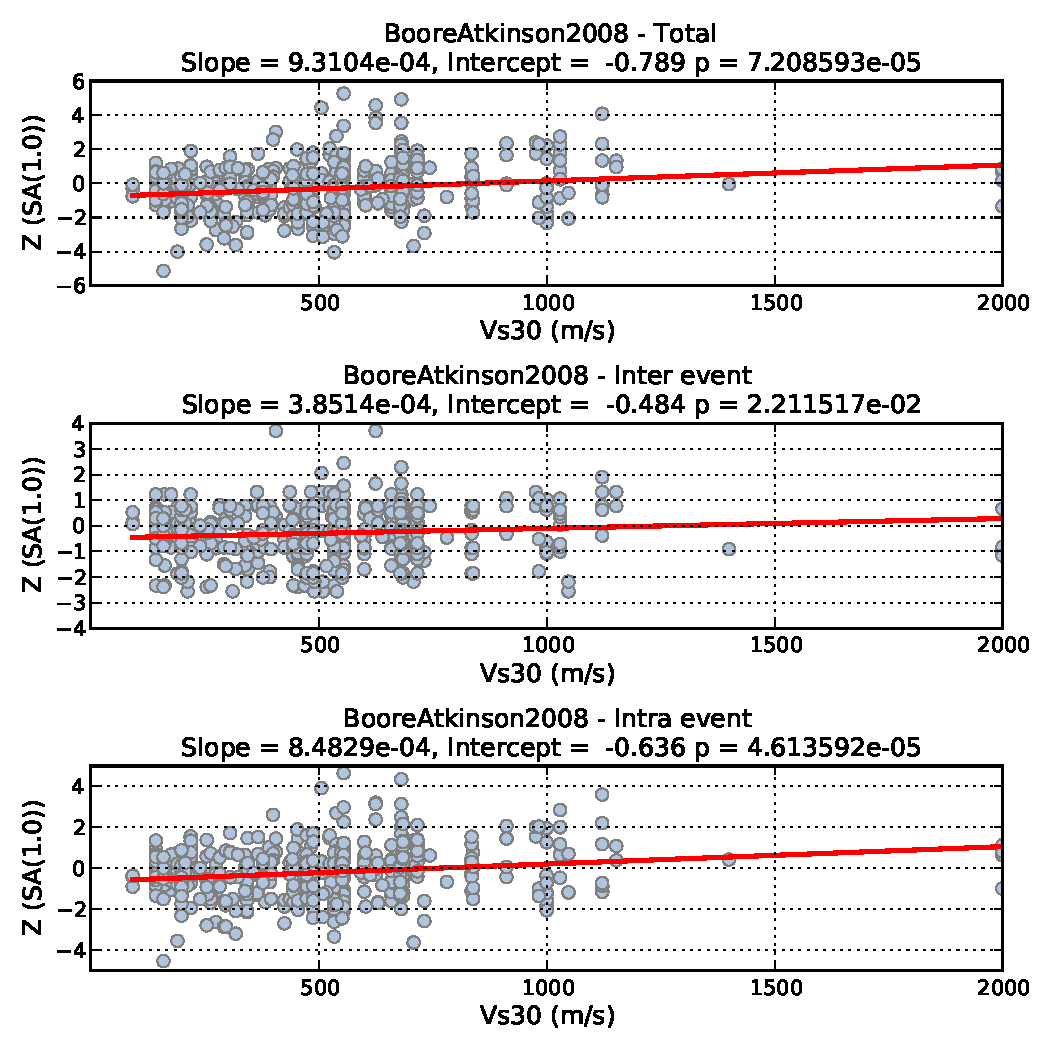
\includegraphics[width=\textwidth]{./figures/residuals/BA2008_Vs30_Sa1.pdf}
      \caption{citeBooreAtkinson2008 model - $Sa \left( {1.0 s} \right)$}
      \label{fig:sa1_vs30_ba2008}
  \end{subfigure}
      \begin{subfigure}[b]{0.49\textwidth}
      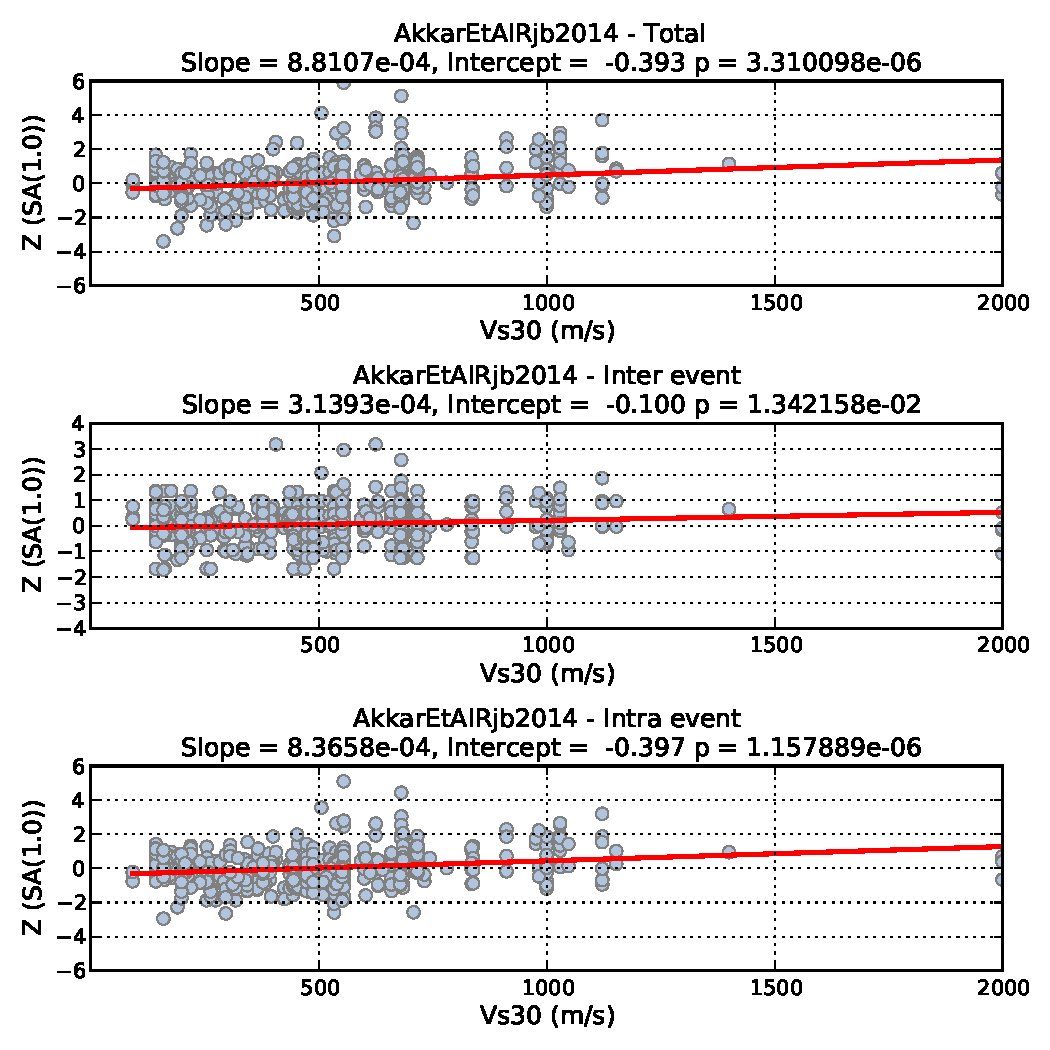
\includegraphics[width=\textwidth]{./figures/residuals/Akkar2014_Vs30_Sa1.pdf}
     \caption{citeAkkarEtAl2014 model - $Sa \left( {1.0 s} \right)$}
      \label{fig:sa1_vs30_akkar2014}
  \end{subfigure}
  \caption{Residual trends with $V_{S30}$ for the observed PGA and $Sa \left( {1.0 s} \right)$ records}
  \label{fig:vs30_resid}
\end{figure}

\subsubsection{Trends with Hypocentral Depth}

Finally, the \verb=rspl= tools contain the method \verb=ResidualWithDepth= to show the trend in the GMPE residuals with \emph{hypocentral} depth. As with the previous residual plotting tools, the commands below will produce plots similar to those shown in Figure \ref{fig:depth_resid}:

 \begin{python}[frame=single]
# Boore & Atkinson (2008)  - PGA
rspl.ResidualWithDepth(resid1,  # Residuals
                      "BooreAtkinson2008",  # GMPE
                      "PGA",   # Intensity Measure
                      filename="path/to/image.png",
                      filetype="png")
# Akkar et al. (2014)  - PGA
rspl.ResidualWithDepth(resid1, "AkkarEtAlRjb2014", "PGA") 
# Boore & Atkinson (2008)  - Sa (1.0)
rspl.ResidualWithDepth(resid1, "BooreAtkinson2008", "Sa(1.0)") 
# Akkar et al. (2014)  - Sa (1.0)
rspl.ResidualWithDepth(resid1, "AkkarEtAlRjb2014", "Sa(1.0)")                         
\end{python}

In this case both GMPEs show statistically significant negative trends in the residual with respect to depth. As expected, it is the inter-event residual where these trends are evident, and that control the trends in the total residual. This indicates that the GMPEs are predicting higher ground motions for deeper events than those observed. For the two GMPEs considered, this result is somewhat expected as neither have an explicit dependence on a depth predictor variable; hence hypocentral depth is within the aleatory variability of the model. 

\begin{figure}[htb]
  \centering
  \begin{subfigure}[b]{0.49\textwidth}
      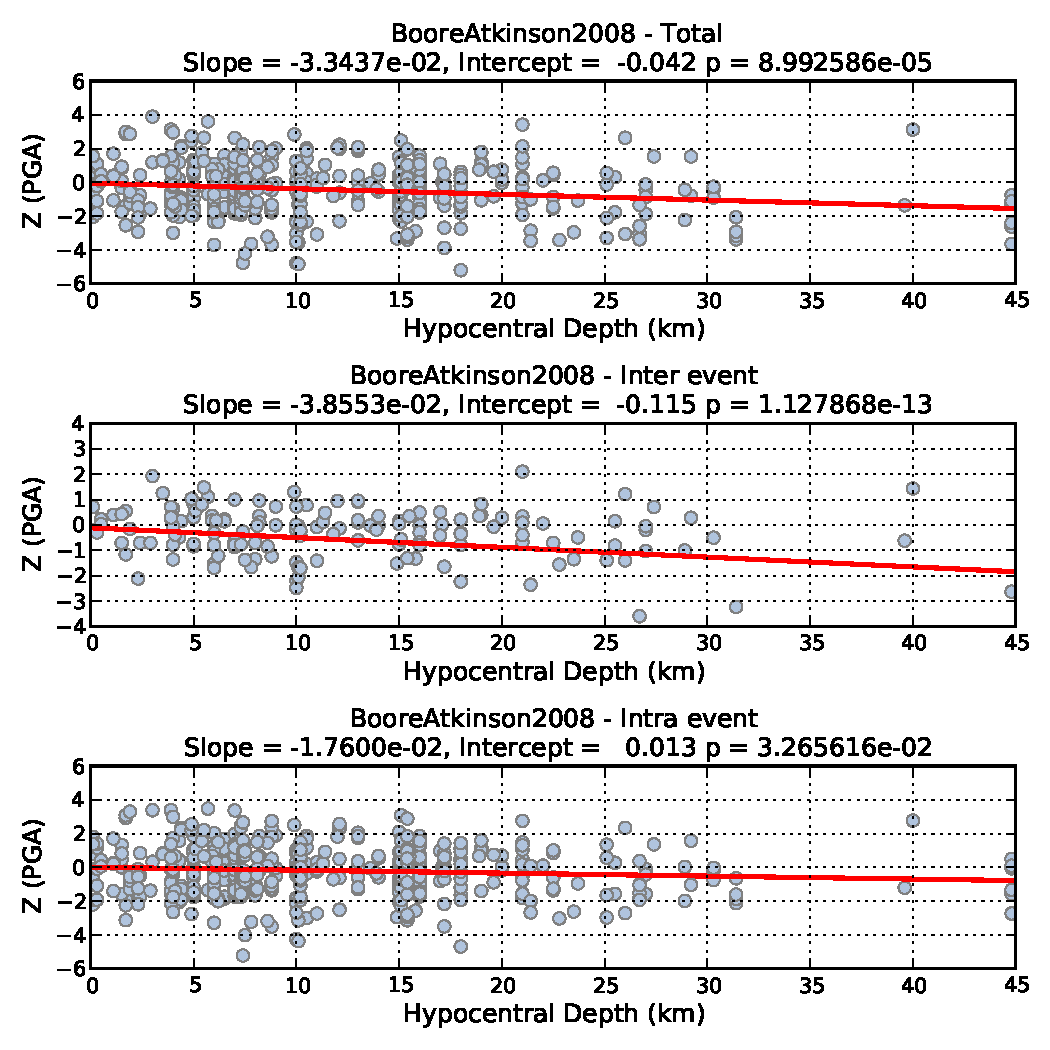
\includegraphics[width=\textwidth]{./figures/residuals/BA2008_HypoDepth_PGA.pdf}
      \caption{citeBooreAtkinson2008 model - PGA}
      \label{fig:pga_depth_ba2008}
  \end{subfigure}
    \begin{subfigure}[b]{0.49\textwidth}
      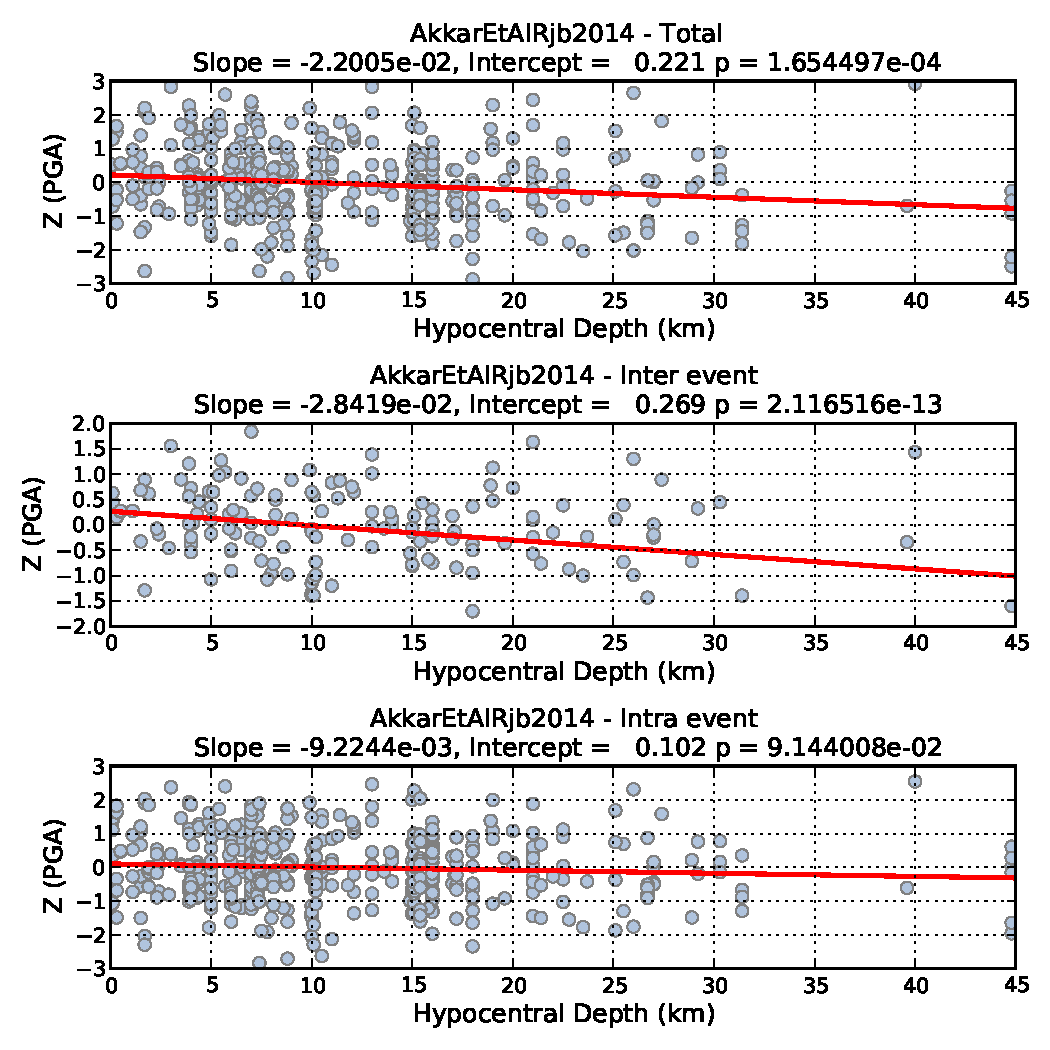
\includegraphics[width=\textwidth]{./figures/residuals/Akkar2014_HypoDepth_PGA.pdf}
      \caption{citeAkkarBommer2010 model - PGA}
      \label{fig:pga_depth_akkar2014}
  \end{subfigure}
    \begin{subfigure}[b]{0.49\textwidth}
      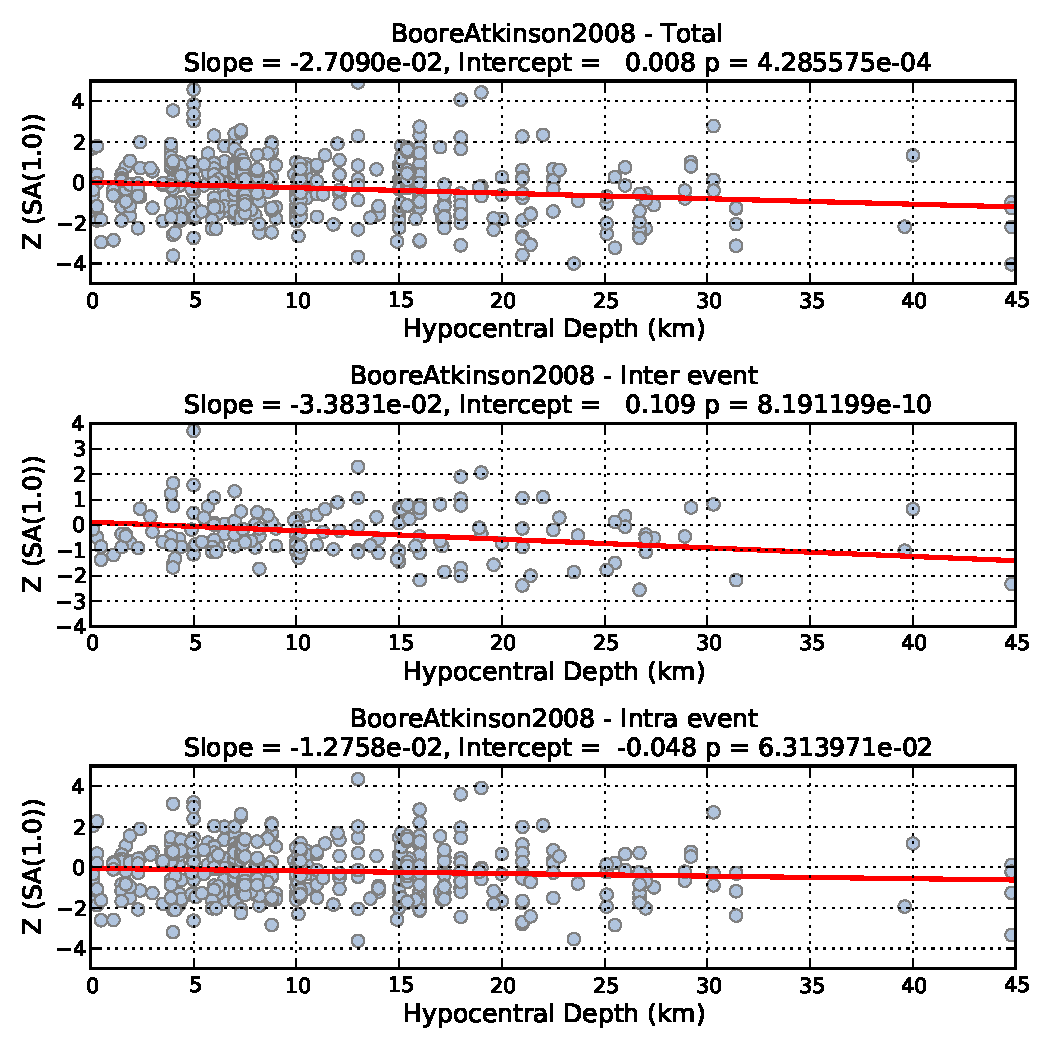
\includegraphics[width=\textwidth]{./figures/residuals/BA2008_HypoDepth_Sa1.pdf}
      \caption{citeBooreAtkinson2008 model - $Sa \left( {1.0 s} \right)$}
      \label{fig:sa1_depth_ba2008}
  \end{subfigure}
      \begin{subfigure}[b]{0.49\textwidth}
      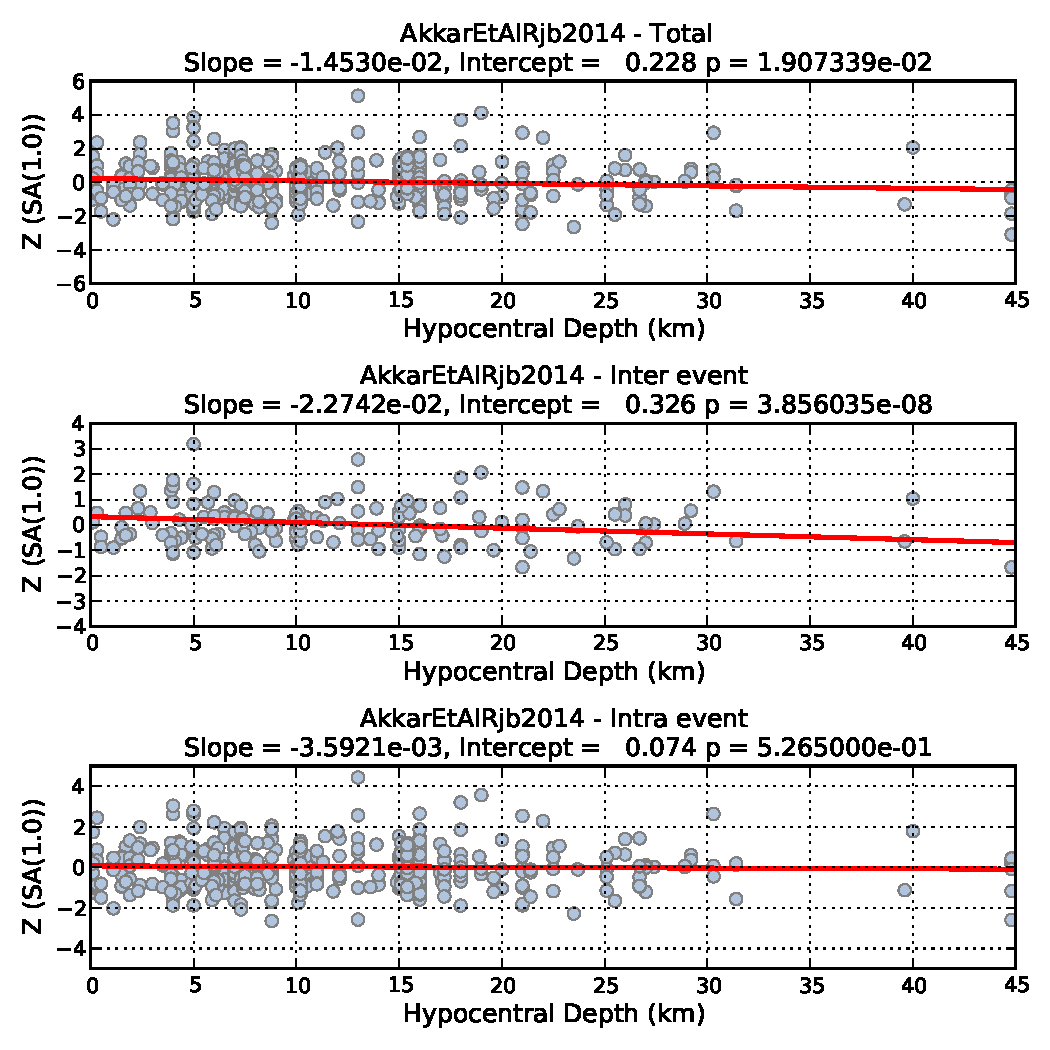
\includegraphics[width=\textwidth]{./figures/residuals/Akkar2014_HypoDepth_Sa1.pdf}
     \caption{citeAkkarEtAl2014 model - $Sa \left( {1.0 s} \right)$}
      \label{fig:sa1_depth_akkar2014}
  \end{subfigure}
  \caption{Residual trends with hypocentral depth for the observed PGA and $Sa \left( {1.0 s} \right)$ records}
  \label{fig:depth_resid}
\end{figure}

\section{Log-likelihood Approach}
\label{sec:llh}

\begin{python}[frame=single]
llh_1 = res.LLH(gmpe_list, imt_list)
llh_1.get_residuals(italy_db_clean)
 Run LLH analysis
llh_values, weights = llh_1.get_loglikelihood_values()
\end{python}

To view the $LLH$ values and weights, it is only necessary to do the following:

\begin{python}
for gmpe in gmpe_list:
    print "LLH(%s) = %12.6f Weight = %12.6f" %(gmpe,
                                               llh_values[gmpe],     
                                               weights[gmpe])
\end{python}

\noindent which, for the GMPEs and the strong motion database considered throughout this chapter, returns an output similar to that below:

\begin{verbatim}
LLH(BooreAtkinson2008) =     3.025793  Weight =     0.175937
LLH(AkkarBommer2010) =     2.559079  Weight =     0.243138
LLH(AkkarCagnan2010) =     2.366239  Weight =     0.277909
LLH(AkkarEtAlRjb2014) =     2.241463  Weight =     0.303015
\end{verbatim}


\section{Euclidean Distance Based Ranking}
\label{sec:edr}

\begin{python}[frame=single]
# EDR analysis
edr1 = res.EDR(gmpe_list, imt_list)
edr1.get_residuals(italy_db_clean)
edr_values = edr1.get_edr_values()
\end{python}

To view the $EDR$ values and weights, it is only necessary to do the following:

\begin{python}
for gmpe in gmpe_list:
    print "EDR(%s) = %8.4f (sqrt(kappa) = %8.4f)" %(gmpe,
        edr_values[gmpe]["EDR"], edr_values[gmpe]["sqrt Kappa"])
\end{python}

\begin{verbatim}
EDR(BooreAtkinson2008) =   1.2163 (sqrt(kappa) =   1.1840)
EDR(AkkarBommer2010) =   1.0990 (sqrt(kappa) =   1.0609)
EDR(AkkarCagnan2010) =   1.3704 (sqrt(kappa) =   1.1308)
EDR(AkkarEtAlRjb2014) =   1.0956 (sqrt(kappa) =   1.0889)
\end{verbatim}

\section{Site Specific Analysis}
\label{sec:site}

%----------------------------------------------------------------------------------------
%	CHAPTER 6
%----------------------------------------------------------------------------------------
\chapterimage{./figures/chapter_head_1.pdf} % Chapter heading image
\chapter{Hazard Applications}
\label{chap:hazard}
\section{Developing GMPE Logic Trees: A ``Good Practice'' Guide}
\label{sec:logic_tree}

(TODO) - If possible I would like some of these issues to be discussed at the meeting.

\section{Conditional Field Simulation}
\label{sec:cond_field}

The extraction of the ground motion residuals from a set of observations also opens up the possibility of implementing another type of calculation that is becoming increasingly common in seismic hazard and risk modelling, and that is conditional random field simulation. These are randomly generated fields of ground motion residuals ($z$) whose values are i) spatially correlated according to a multivariate Gaussian distribution, and ii) conditioned upon observed (known) values of the residual. This type of analysis can be critical in characterising the uncertainty in ``ShakeMaps'' (i.e. field of ground motion generated from an observed event), which in turn can provide insights into the distribution of expected or, if applied \emph{a posteriori}, observed losses \citep[e.g.][]{Park_etal2007, Crowley_etal2008b, Stafford2012}.

It has been well-established from observations of densely recorded earthquakes, that ground motion residuals are spatially correlated when stations are separated by distances typically on the order of a few tens of kilometres \citep{Jayaram2009}. Given the assumption of lognormality in the GMPEs, it is has also been demonstrated appropriate to model the spatial correlation in ground motion residual between two or more sites using a multivariate Gaussian distribution \citep{JayaramBaker2009}. The coeffiecient of correlation between two sites separated by a distance $h$ ($\rho \left( h \right)$) is shown to decay exponentially with distance such that:

\begin{equation}
\rho \left( h \right) = \exp \left( {\frac{-a\left(T\right) h}{b \left(T\right)}} \right)
\end{equation}

\noindent where $a\left( T \right)$ and $b\left( T \right)$ control the shape of the decay and are dependent on the period of ground motion under consideration. One such model of spatial correlation, which we shall use in this example, is that of cite \cite{Jayaram2009}:

\begin{equation}
\rho \left( h \right) = \exp\left( {\frac{-3h}{b \left( T \right)}} \right) \quad \text{where} \quad b \left( T \right) = \begin{cases}\begin{cases}
8.5 + 17.2 T \text{ ``Case 1'' } & T < 1\ s\\
40.7 - 15.0 T \text{ ``Case 2'' } & T < 1\ s\end{cases}&\\
\qquad 22.0 + 3.7 T \qquad\qquad\quad T \geq 1\ s&
\end{cases}
\label{eq:jayarambaker}
\end{equation}

Consider a set of correlated random variables distributed according to a multivariate Gaussian distribution with a mean of zero and a standard deviation of unity ($\mathbf{X} = \left[ {X_1, X_2, \ldots , X_N} \right]$) and with a positive definite covariance matrix given by $\mathbf{C}$. A randomly generated sample of values can be generated via:

\begin{equation}
\mathbf{X} = \mathbf{\mu} + \mathbf{LU}
\end{equation}

\noindent where $\mathbf{\mu}$ is the mean values of the field (in this case a zero-vector $\mathbf{0}$), $\mathbf{U}$ is a sample of independent normally distributed random variates and $\mathbf{L}$ is the lower matrix defined by $\mathbf{LL^T} = \mathbf{C}$, which is obtained by Cholesky factorisation of the covariance matrix. This assumes that values of $\mathbf{X}$ are unknown \emph{a priori}, as might be the case if considering spatially correlated fields of ground motion residuals for some as yet unrecorded event. The ability to generate spatially correlated fields in this manner is supported directly by OpenQuake.

When considering a recorded event it is possible to partition the ground motion field into those locations for which the GMPE residual is known ($\mathbf{X_{OBS}}$), and those for which it is unknown ($\mathbf{X_{UNK}}$). Given the locations of both the known and unknown values the covariance matrices can be formed where $\mathbf{C_{11}}$ is the covariance of the known residuals, $\mathbf{C_{22}}$ the covariance of the unknown locations and $\mathbf{C_{12}}$ and $\mathbf{C_{21}}$ the covariance matrices considering the distance between the known and unknown locations. In the case of a multivariate standard normal distribution, the distribution of residuals at both locations can be depicted as:

\begin{equation}
\begin{bmatrix}\mathbf{X_{OBS}}\\ \hline \mathbf{X_{UNK}}\end{bmatrix} \sim N_M \left( {\begin{bmatrix}\mathbf{0} \\ \hline \mathbf{0}\end{bmatrix}, \left[ {\begin{array}{c|c}\mathbf{C_{11}} & \mathbf{C_{12}} \\ \hline \mathbf{C_{21}} & \mathbf{C_{22}}\end{array}}\right]}\right)
\end{equation}

\noindent which is arranged to give the distribution of residuals at the unknown locations, conditional upon the known residuals:
\begin{equation}
\left[ {\mathbf{X_{UNK}} | \mathbf{X_{OBS}}} \right] \sim N_M \left( {\left[ {\mathbf{C_{21}C_{11}^{-1}X_{OBS}}} \right], \left[ {\mathbf{C_{22}} - \mathbf{C_{21}C_{11}^{-1}C_{12}}}\right]}\right)
\end{equation}

From this model it is then possible to simulate random fields of GMPE residuals conditioned upon observed residuals. This functionality is not directly supported in OpenQuake, as it requires a mean by which the observed residuals can be characterised using the desired GMPE. As has been shown in Chapter \ref{chap:residuals}, however, the GMPE-SMTK does exactly this. Therefore it becomes possible to use the GMPE-SMTK, in conjunction with OpenQuake, to produce multiple fields of spatially correlated ground motions that are conditional upon a set of known observations. For this purpose we include a set of tools in a module called \verb=smtk.hazard.conditional_simulation=, which we shall import as, and subsequently refer to as, \verb=csim=

\begin{python}
import smtk.hazard.conditional_simulation as csim
\end{python}

\subsection{Example of Conditional Simulation: L'Aquila}

In the following example we consider a set of 15 records taken from the L'Aquila earthquake. In the current example these records have been put into a GMPE-SMTK database on the path \verb=/data/LAquila_Database/=, following the approach described in section \ref{sec:hdf5}. The first step in this process is to load the database and calculate the ground motion residuals:

\begin{python}[frame=single]
import cPickle
from smtk.residuals.gmpe_residuals import Residuals
# Load the database 
import cPickle
db1 = cPickle.load(open("./data/LAquila_Database/metadatafile.pkl",
                        "r"))
\end{python}

In this example we shall consider only the \cite{Akkar_etal2014} GMPE, and just two intensity measures: PGA and $Sa \left( {1.0s} \right)$:

\begin{python}[frame=single]
gmpe_list = ["AkkarEtAlRjb2014"]
imts = ["PGA", "SA(0.2)", "SA(1.0)"]
# Calculate the residuals
resid1 = Residuals(gmpe_list, imts)
resid1.get_residuals(db1)
\end{python}

We may be interested to observe the distance trend in these residuals. This is generated using the tools described in chapter \ref{chap:residuals}, and can be seen in Figure \ref{fig:laquila_resid_distance}.

\begin{figure}[htb]
  \centering
  \begin{subfigure}[b]{0.49\textwidth}
      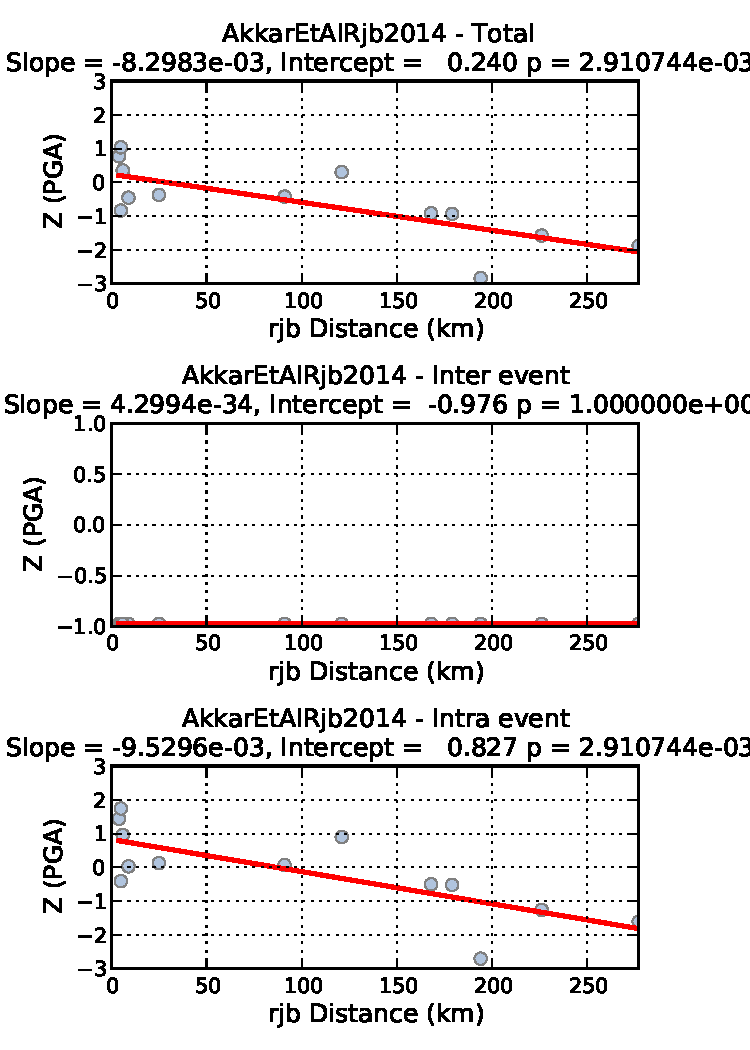
\includegraphics[width=\textwidth]{./figures/hazard/LAquila_Residuals_with_distance.pdf}
      \caption{PGA}
      \label{fig:laquila_resid_pga}
  \end{subfigure}
    \begin{subfigure}[b]{0.49\textwidth}
      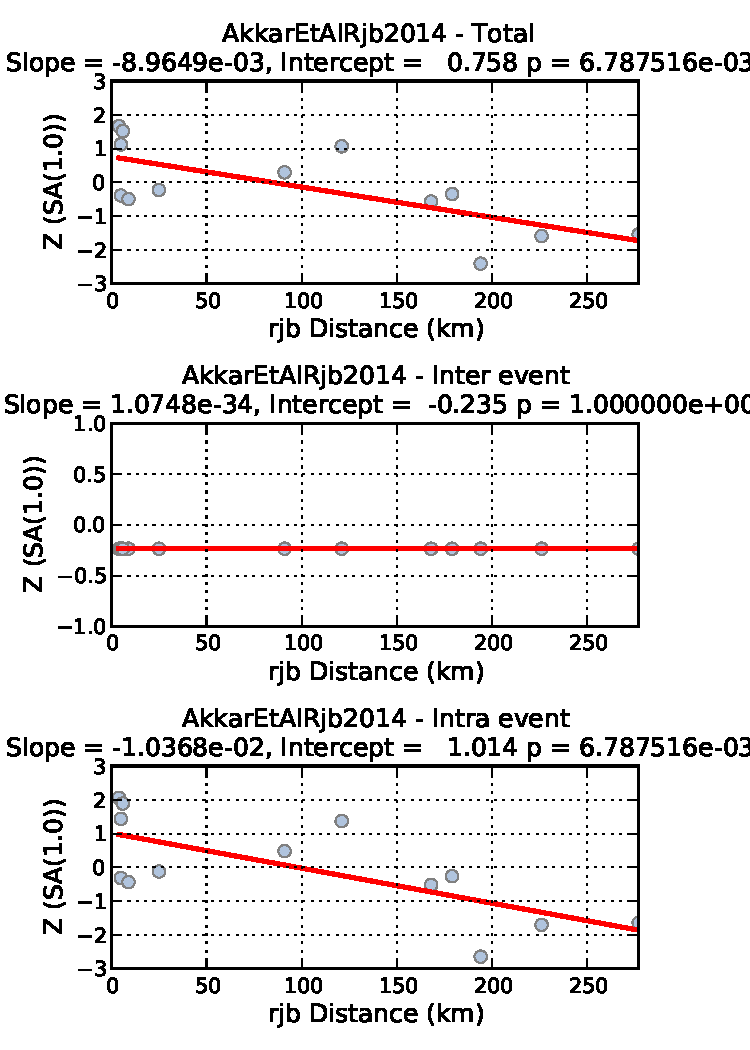
\includegraphics[width=\textwidth]{./figures/hazard/LAquila_Residuals_with_distance_sa1.pdf}
      \caption{$Sa \left( {1.0 s} \right)$ }
      \label{fig:laquila_resid_sa1}
  \end{subfigure}
  \caption{Residual trends with distance for the L'Aquila ground motion residuals}
  \label{fig:laquila_resid_distance}
\end{figure}

Here we see that for both PGA and $Sa \left( {1.0 s} \right)$ the inter-event residual is moderately negative (-0.976 for PGA and -0.235 for $Sa \left( {1.0 s} \right)$), and we observe a clear trend that the ground motions from this earthquake attenuated to a greater extent than that predicted by the GMPE. 

In the present case we have a model of the finite extent of the earthquake rupture. We put this rupture into an OpenQuake xml format\footnote{More information on the OpenQuake scenario rupture format can be found in \cite{crowley2013}}, as shown below, and save it in the file \verb=laquila_rupture.xml=.

\begin{verbatim}
<?xml version='1.0' encoding='utf-8'?>
<nrml xmlns:gml="http://www.opengis.net/gml"
      xmlns="http://openquake.org/xmlns/nrml/0.4">
    <simpleFaultRupture>
        <magnitude>6.3</magnitude>
        <rake>-98.0</rake>
        <hypocenter lon="13.38" lat="42.3476" depth="9.3"/>
        <simpleFaultGeometry>
                <gml:LineString>
                    <gml:posList>
                        13.3976 42.4371
                        13.5571 42.3012
                    </gml:posList>
                </gml:LineString>
            <dip>50.0</dip>
            <upperSeismoDepth>0.8</upperSeismoDepth>
            <lowerSeismoDepth>12.69</lowerSeismoDepth>
        </simpleFaultGeometry>
    </simpleFaultRupture>
</nrml>
\end{verbatim}

With the use of the OpenQuake hazardlibrary and Python's \verb=Matplotlib= plotting tools we can visualise the spatial trend in the residuals. Firstly we load in the rupture. The \verb=csim= module contains the method \verb=build_rupture_from_file=, which will load in the rupture:

\begin{python}
rupture_file = "laquila_rupture.xml"
rupture = csim.build_rupture_from_file(rupture_file)
\end{python}

For plotting it is convenient to define the outline of the surface projection of the rupture as a simple polygon:

\begin{python}
# Import the OpenQuake polygon class
from openquake.hazardlib.geo.polygon import Polygon
rupture_outline = Polygon([rupture.surface.top_left,
                           rupture.surface.top_right,
                           rupture.surface.bottom_right,
                           rupture.surface.bottom_left,
                           rupture.surface.top_left])
\end{python}

The next step is to take the database and return its locations as an instance of the class \verb=openquake.hazardlib.site.SiteCollection=. This can be done using the method within the database class (\verb=GroundMotionDatabase=) called \verb=get_site_collection=

\begin{python}
observed_sites = db1.get_site_collection()
\end{python}

The plot of the spatial distribution of residuals of PGA with respect to the rupture location is shown in Figure \ref{fig:laquila_spatial_resid}. This can be generated using the Python code below:

\begin{python}[frame=single]
# Import the Matplotlib library
import matplotlib.pyplot as plt
# Extract the PGA residuals
pga_residuals = resid1.residuals["AkkarEtAlRjb2014"]["PGA"]["Intra event"]
plt.figure(figsize=(10,8))
# Plot the rupture
plt.plot(rupture_outline.lons, rupture_outline.lats, "r-")
# Plot the reisduals
plt.scatter(observed_sites.lons, observed_sites.lats, 
            s=40,
            c=pga_residuals, 
            norm=Normalize(vmin=-3.0, vmax=3.0))
plt.title("PGA Observed Intra-event Residual", fontsize=16)
plt.colorbar()
plt.xlabel("Longitude", fontsize=14)
plt.ylabel("Latitude", fontsize=14)
\end{python}

\begin{figure}[htb]
  \centering
  \begin{subfigure}[b]{\textwidth}
      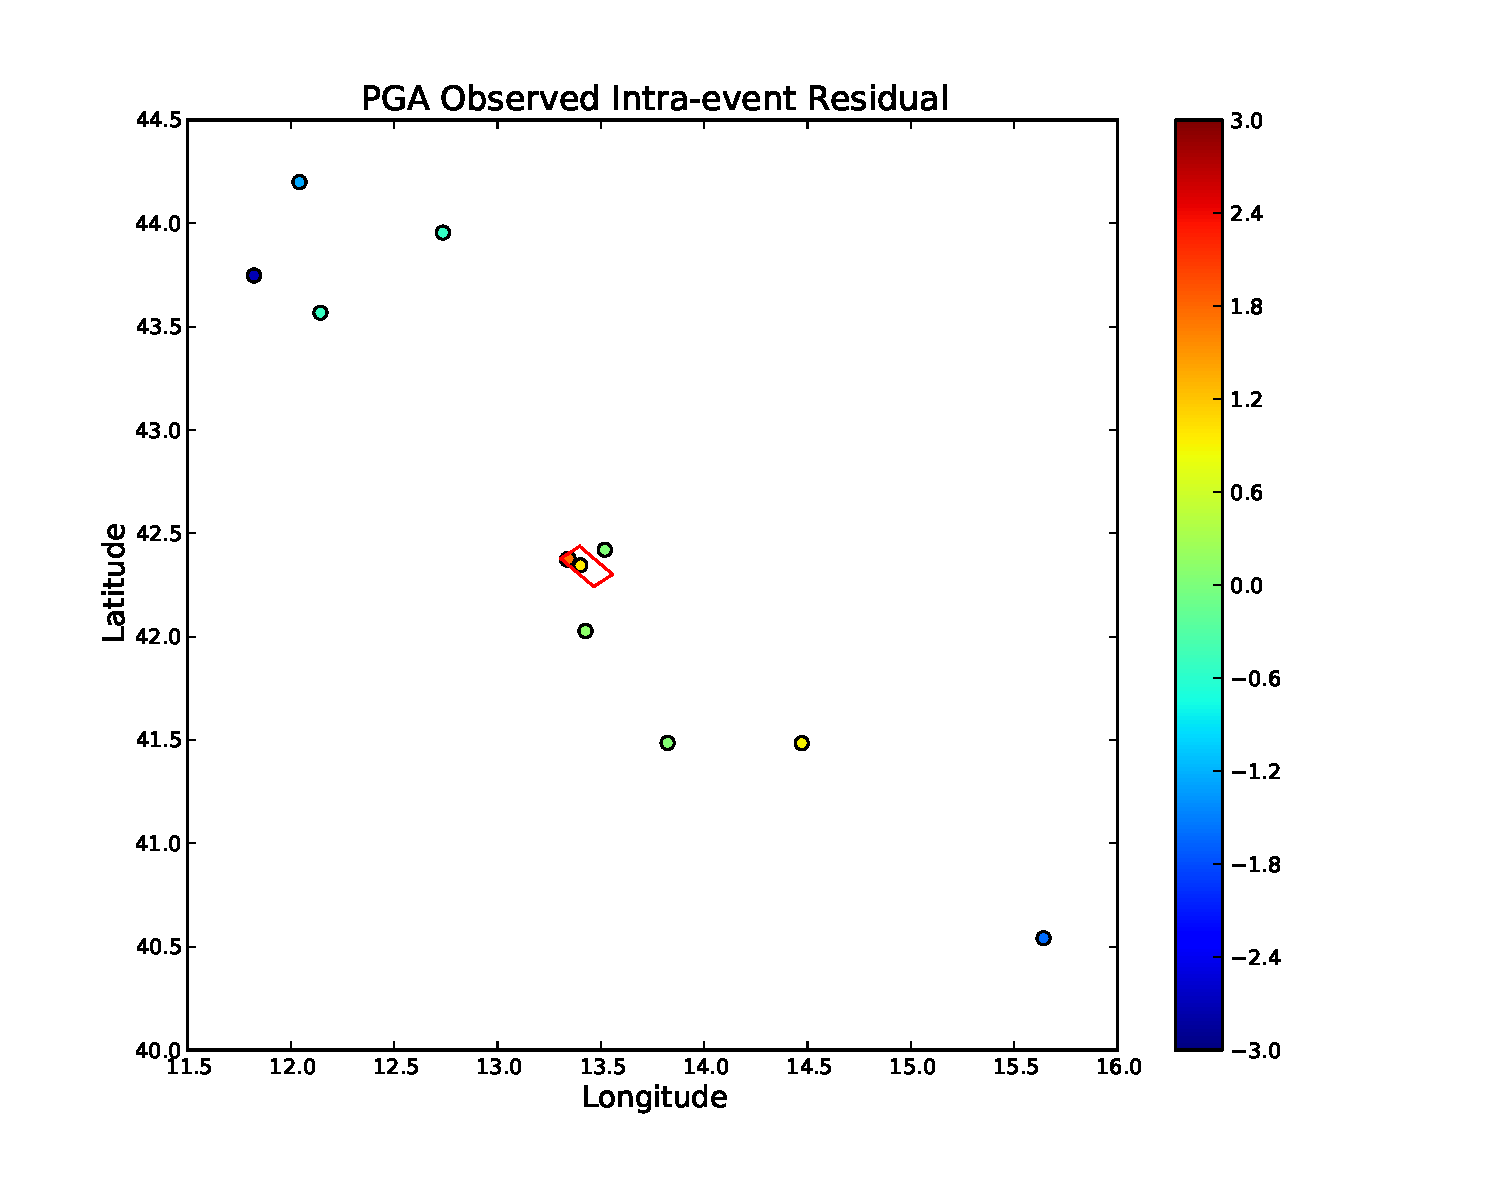
\includegraphics[trim=14mm 14mm 14mm 14mm, clip, width=0.65\textwidth]{./figures/hazard/LAquila_Observed_IntraEvent_Resid.pdf}
      \label{fig:laquila_spatial_resid_pga}
  \end{subfigure}
    \begin{subfigure}[b]{\textwidth}
      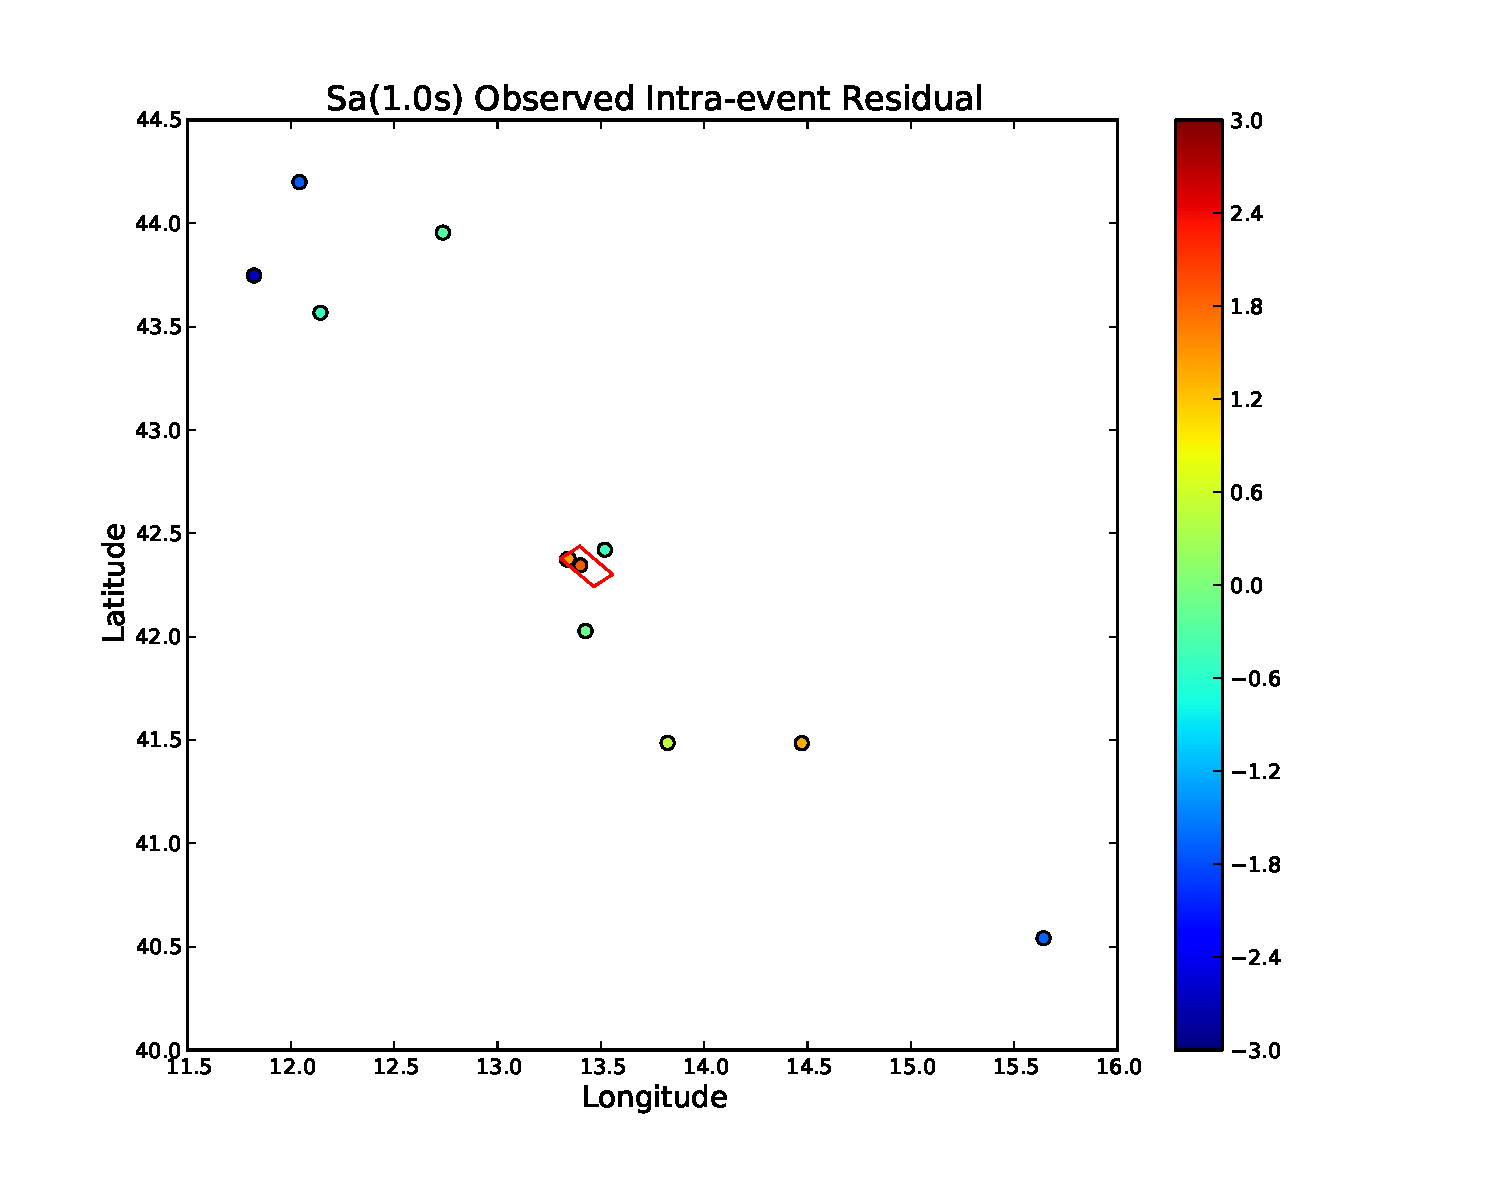
\includegraphics[trim=14mm 14mm 14mm 14mm, clip, width=0.65\textwidth]{./figures/hazard/LAquila_Observed_IntraEvent_Resid_sa1.pdf}
      \label{fig:laquila_spatial_resid_sa1}
  \end{subfigure}
  \caption{Distribution of intra-event residuals for the L'Aquila ground motion records. The surface projection of the L'Aquila rupture is shown in red.}
  \label{fig:laquila_spatial_resid}
\end{figure}

Figure \ref{fig:laquila_spatial_resid} helps understand the residual distribution further as we observed that for both intensity measures there is a small cluster of strongly positive residuals in the very near-field of the fault (due to directivity effects).

If we want to generate a spatially correlated random field of observations around the L'Aquila area, we can use the observed GMPE residuals and the spatial correlation model in equation \ref{eq:jayarambaker} to generate a realisation of a field of possible residuals. In the present example we have created a regularly spaced grid of ``target'' (i.e. unknown sites) with known soil properties. We assume this has been created as an instance of the \verb=openquake.hazardlib.site.SiteCollection= class, and we call this variable \verb=unknown_sites=. To generate a 10 random fields of spatially correlated residuals conditioned upon a set of observations we can use the \verb=csim= method \verb=conditional_simulation= as follows:

\begin{python}
# Generate fields of conditioned on the PGA residuals
output_resid_pga = csim.conditional_simulation(observed_sites,
                                               pga_residuals,
                                               unknown_sites,
                                               "PGA",
                                               nsim=10)
# Generate fields of conditioned on the Sa (1.0) residuals
output_resid_sa1 = csim.conditional_simulation(observed_sites,
                                               pga_residuals,
                                               unknown_sites,
                                               "SA(1.0)",
                                               nsim=10)
\end{python}
\noindent The output will be an array of shape $N_{SITES} \times N_{SIMULATIONS}$, where $N_{SITES}$ is the number of unknown sites and $N_{SIMULATIONS}$ the number of desired random fields (10 in this example). For a field located close to the rupture, the spatially correlated residuals are shown for both intensity meausres in Figures \ref{fig:laquila_epsilon_pga} and Figures \ref{fig:laquila_epsilon_sa1} respectively.  

\begin{figure}[htb]
	\centering
		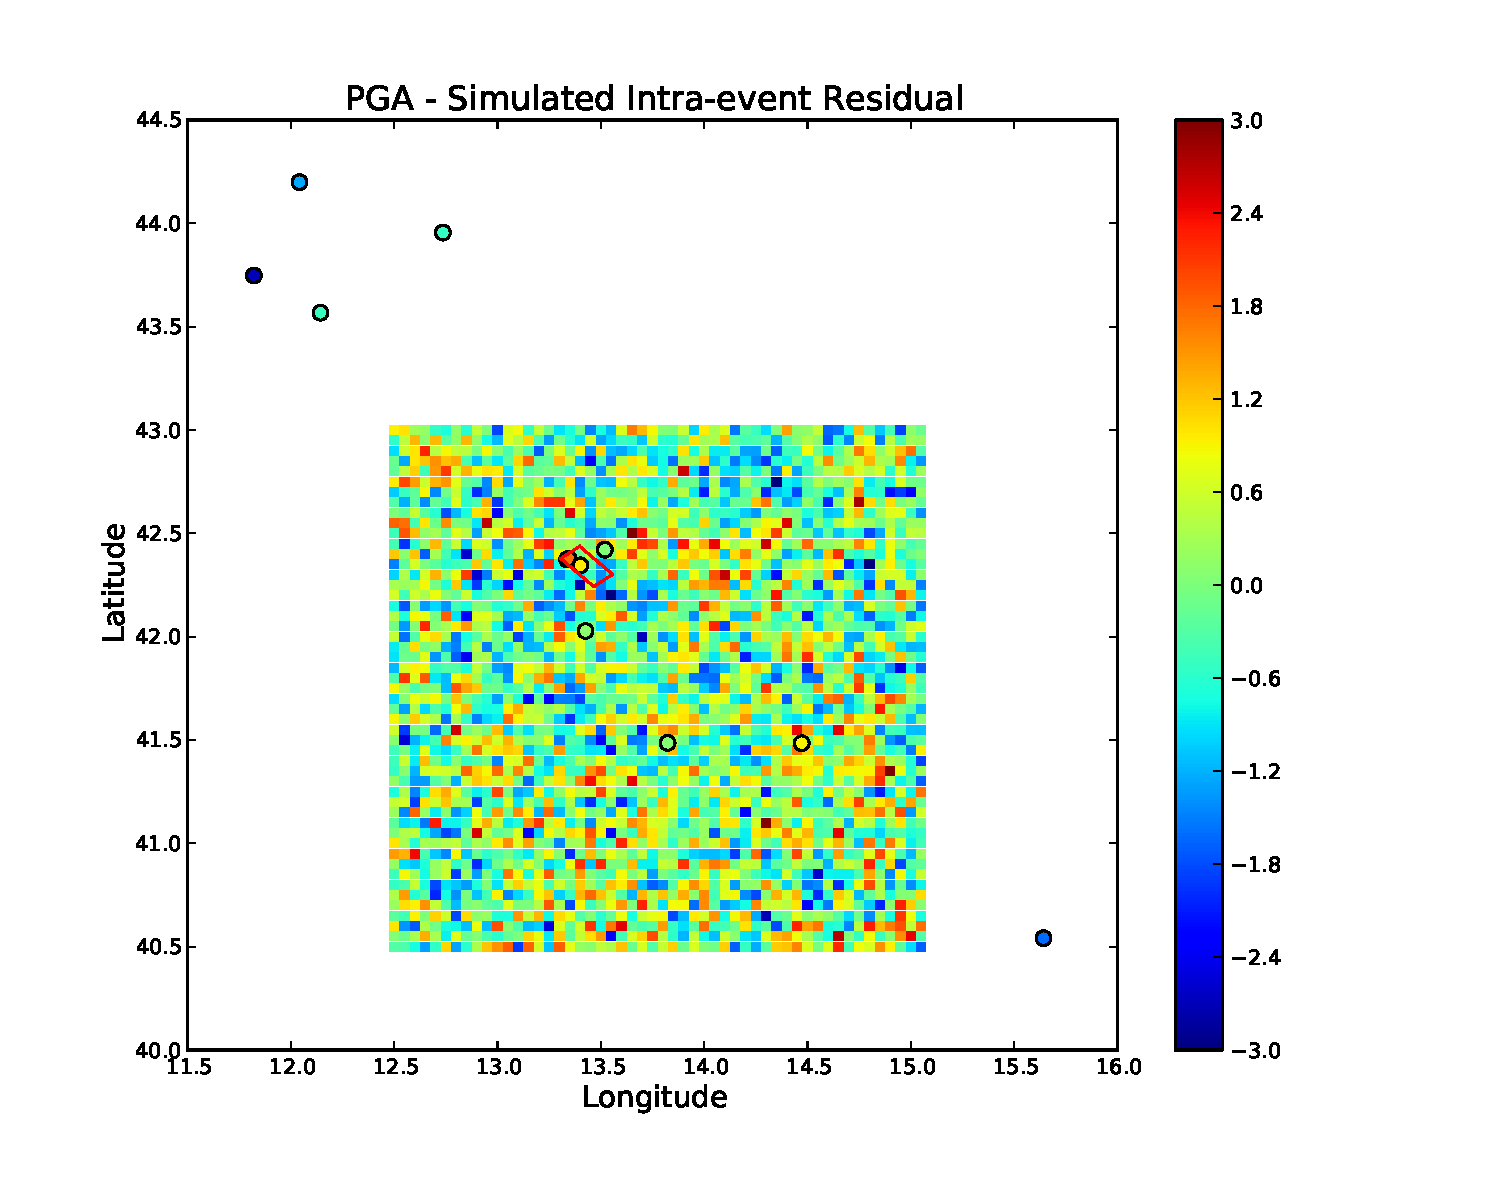
\includegraphics[trim=10mm 10mm 10mm 10mm, clip, width=0.8\textwidth]{./figures/hazard/LAquila_Simulated_Epison_PGA.pdf}
	\caption{Random field of PGA ground motion residuals conditioned upon observed residuals (circles) in the L'Aquila region}
	\label{fig:laquila_epsilon_pga}
\end{figure}
\begin{figure}[htb]
	\centering
		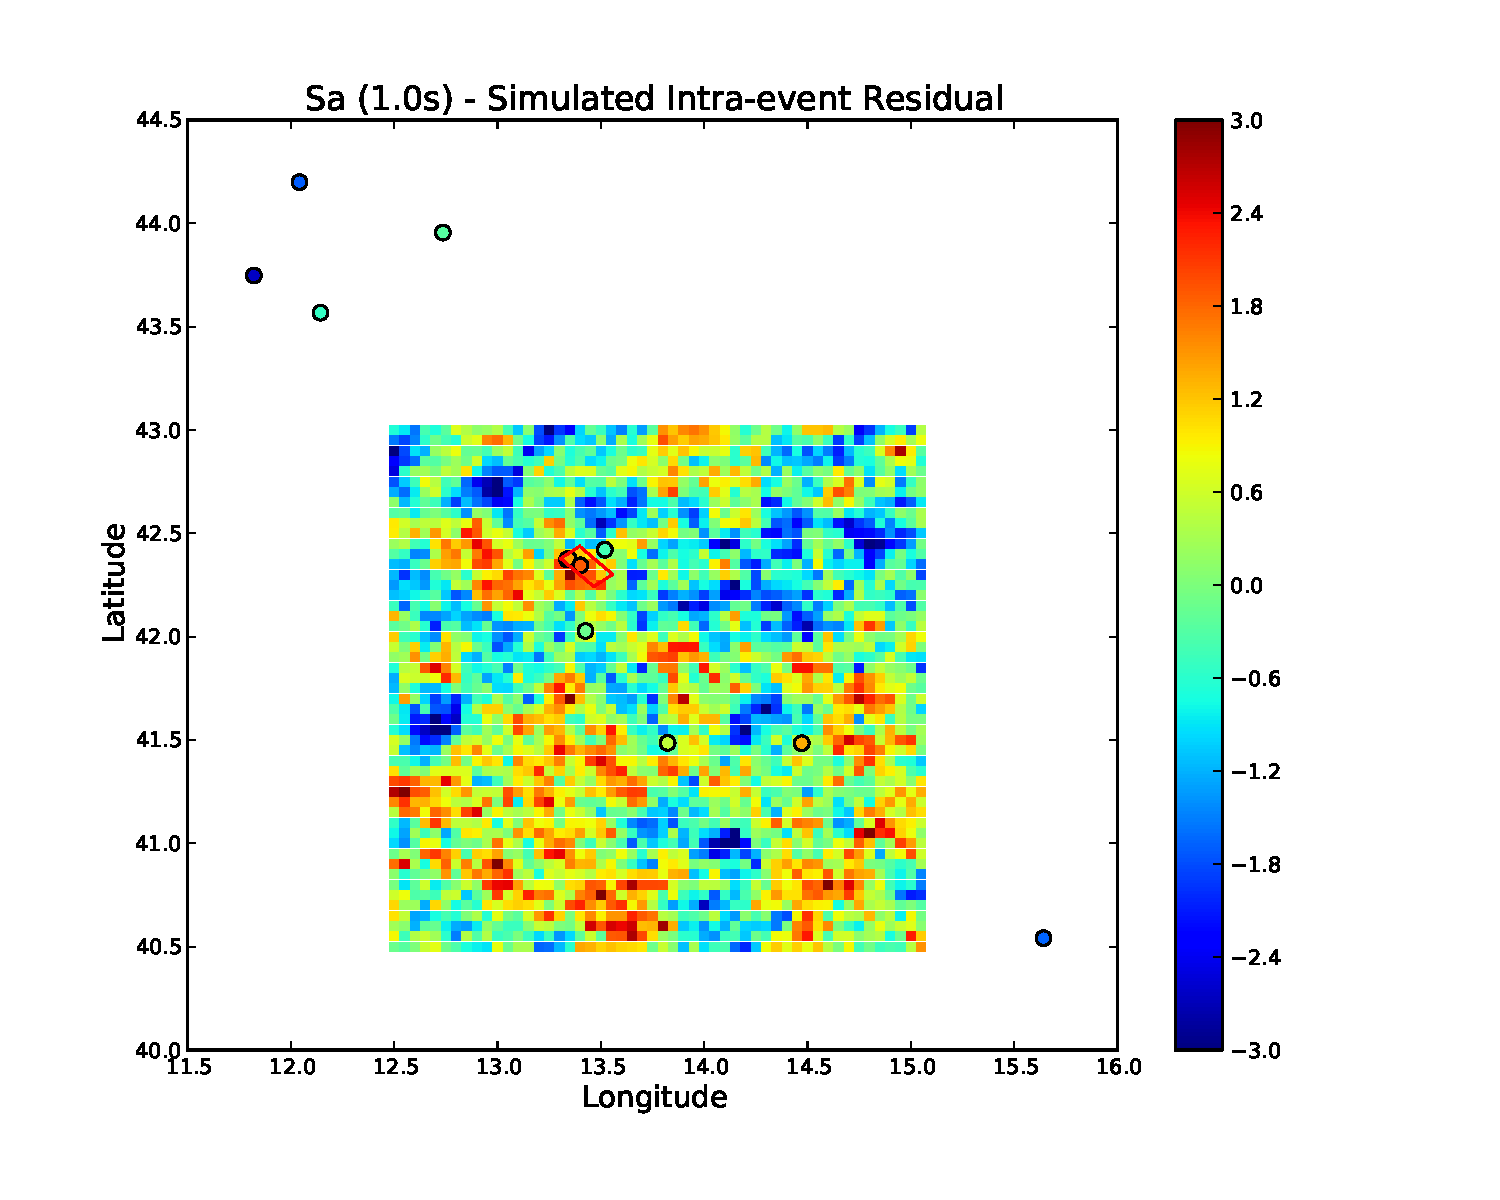
\includegraphics[trim=10mm 10mm 10mm 10mm, clip, width=0.8\textwidth]{./figures/hazard/LAquila_Simulated_Epsilon_Sa1.pdf}
	\caption{Random field of $Sa \left( {1.0 s} \right)$ ground motion residuals conditioned upon observed residuals (circles) in the L'Aquila region}
	\label{fig:laquila_epsilon_sa1}
\end{figure}

The spacing of this particular field is approximately 5 km. The typical correlation length (i.e. the distance at which $\rho \left( h \right)$ drops below 0.05) of PGA is on the order of approaximately 10 to 15 km. Given the exponential model it is evident that for PGA the spatial correlation is not so significant at this resolution. For $Sa \left( {1.0 s} \right)$ the correlation length may be on the order of 30 to 40 km; hence both the spatial correlation and the effects of the conditioning are visible clearly in Figure \ref{fig:laquila_epsilon_sa1}. Particular attention should be paid to the area of strong positive residuals in the near-field of the rupture.

The \verb=csim= tools contain a general method to implement much of the process outlined previously. This method is called \verb=get_conditional_gmfs= and its usage is illustrated below:

\begin{python}
gmfs = csim.get_conditional_gmfs(db1,
                                 rupture, 
                                 sites=unknown_sites, 
                                 gsims=["AkkarEtAlRjb2014"],
                                 imts=["PGA", "SA(1.0)"],
                                 number_simulations=5,
                                 truncation_level=3.0)
\end{python}
The above command requires as input:
\begin{enumerate}
\item The database of observed ground motions for the rupture
\item The loaded rupture model
\item The target sites as an instance of the \verb=SiteCollection= class
\item The list of GMPEs
\item The list of intensity measures
\item The number of simulations
\item The number of standard deviations at which to truncate the residuals.
\end{enumerate}

The following code snippet can be used to generate the full simulated ground motion field, similar to the examples shown in Figures \ref{fig:laquila_field_pga} and \ref{fig:laquila_field_sa1}:

\begin{python}[frame=single]
# Get one of the PGA fields from the Akkar et al GMPe
pga_field = gmfs["AkkarEtAlRjb2014"]["PGA"][:, 0]
# Setup the figure
plt.figure(figsize=(10,8))
plt.plot(rupture_outline.lons, rupture_outline.lats, "r-")
# Plot the fields
plt.scatter(unknown_sites.lons, unknown_sites.lats, 
            s=50,
            c=pga_field,
            marker="s",
            edgecolor="None",
            norm=LogNorm(vmin=0.001, vmax=1))
plt.xlim(12.5, 15.0)
plt.ylim(40.5, 43.0)
plt.title("PGA (g) - Conditional Random Field", fontsize=18)
plt.colorbar()
plt.xlabel("Longitude", fontsize=14)
plt.ylabel("Latitude", fontsize=14)
\end{python}

\begin{figure}[htb]
	\centering
		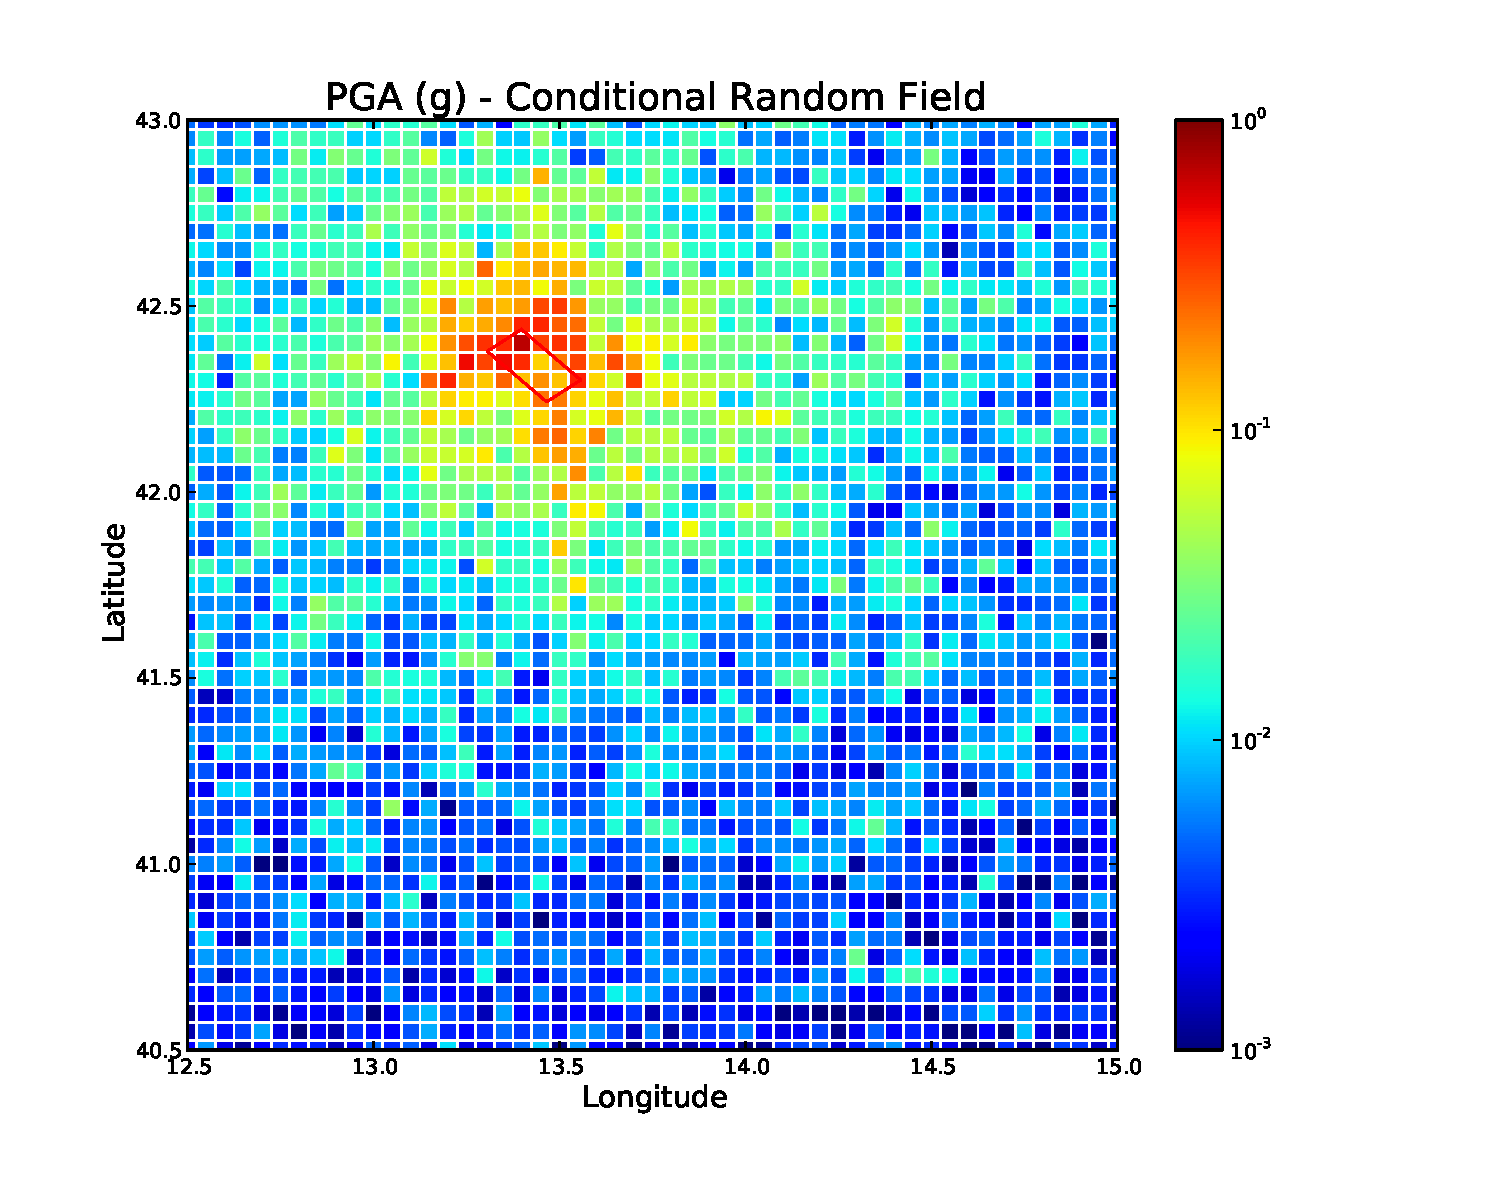
\includegraphics[trim=10mm 10mm 10mm 10mm, clip, width=0.8\textwidth]{./figures/hazard/LAquila_Conditional_Field_PGA.pdf}
	\caption{PGA ground motion field conditioned upon the ground motion residuals conditioned upon observed ground motions from the L'Aquila (2009) earthquake}
	\label{fig:laquila_field_pga}
\end{figure}
\begin{figure}[htb]
	\centering
		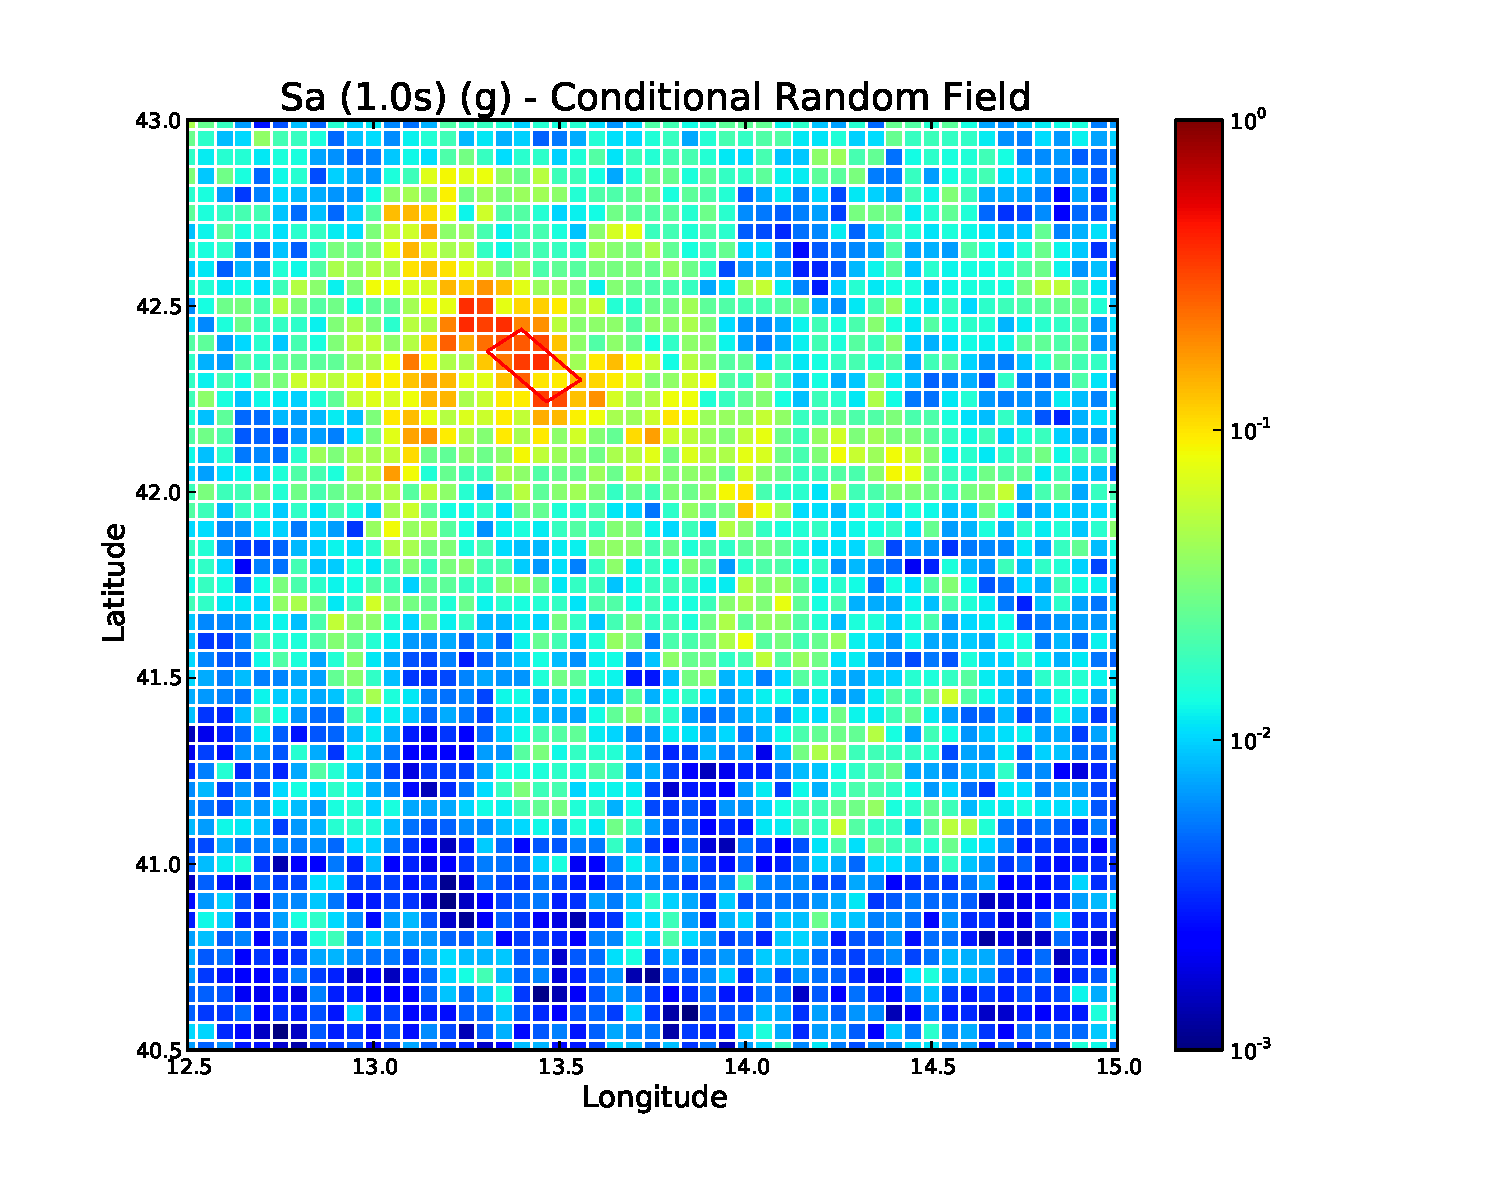
\includegraphics[trim=10mm 10mm 10mm 10mm, clip, width=0.8\textwidth]{./figures/hazard/LAquila_Conditional_Field_Sa1.pdf}
	\caption{$Sa \left( {1.0 s} \right)$ ground motion field conditioned upon the ground motion residuals conditioned upon observed ground motions from the L'Aquila (2009) earthquake}
	\label{fig:laquila_field_sa1}
\end{figure}



%----------------------------------------------------------------------------------------
%	BIBLIOGRAPHY
%----------------------------------------------------------------------------------------
\chapter*{Bibliography}
\addcontentsline{toc}{chapter}{\textcolor{ocre}{Bibliography}}
\section*{Books}
\addcontentsline{toc}{section}{Books}
\printbibliography[heading=bibempty,type=book]
\section*{Articles}
\addcontentsline{toc}{section}{Articles}
\printbibliography[heading=bibempty,type=article]
\section*{Other Sources}
\addcontentsline{toc}{section}{Reports}
\printbibliography[heading=bibempty,nottype=book,nottype=article]


%----------------------------------------------------------------------------------------
%	INDEX
%----------------------------------------------------------------------------------------

\cleardoublepage
\phantomsection
\setlength{\columnsep}{0.75cm}
\addcontentsline{toc}{chapter}{\textcolor{ocre}{Index}}
\printindex
\printglossary

%----------------------------------------------------------------------------------------

\end{document}